\documentclass[a4paper,10pt]{report}

% PyTOUGH user's guide
\usepackage{lmodern}
\usepackage[T1]{fontenc}
\usepackage{framed,color}
\definecolor{shadecolor}{gray}{0.9}
\usepackage[authoryear,round]{natbib}   % for references
\usepackage[hmargin=3.5cm]{geometry} % change margin
\usepackage{rotating} % for sideways tables
\usepackage[a4paper=true]{hyperref}
\usepackage{longtable}

\hypersetup{
  pdftitle = PyTOUGH User's Guide,
  pdfauthor = Adrian Croucher,
  colorlinks = true, % Colours links instead of ugly boxes
  urlcolor = blue, % Colour for external hyperlinks
  linkcolor = blue, % Colour of internal links
  citecolor = red % Colour of citations
}

%------------------------------------------------------------------------
\begin{document}

\begin{titlepage}

\begin{center}

\bigskip\

\textbf{\Huge{PyTOUGH user's guide}}

\bigskip\

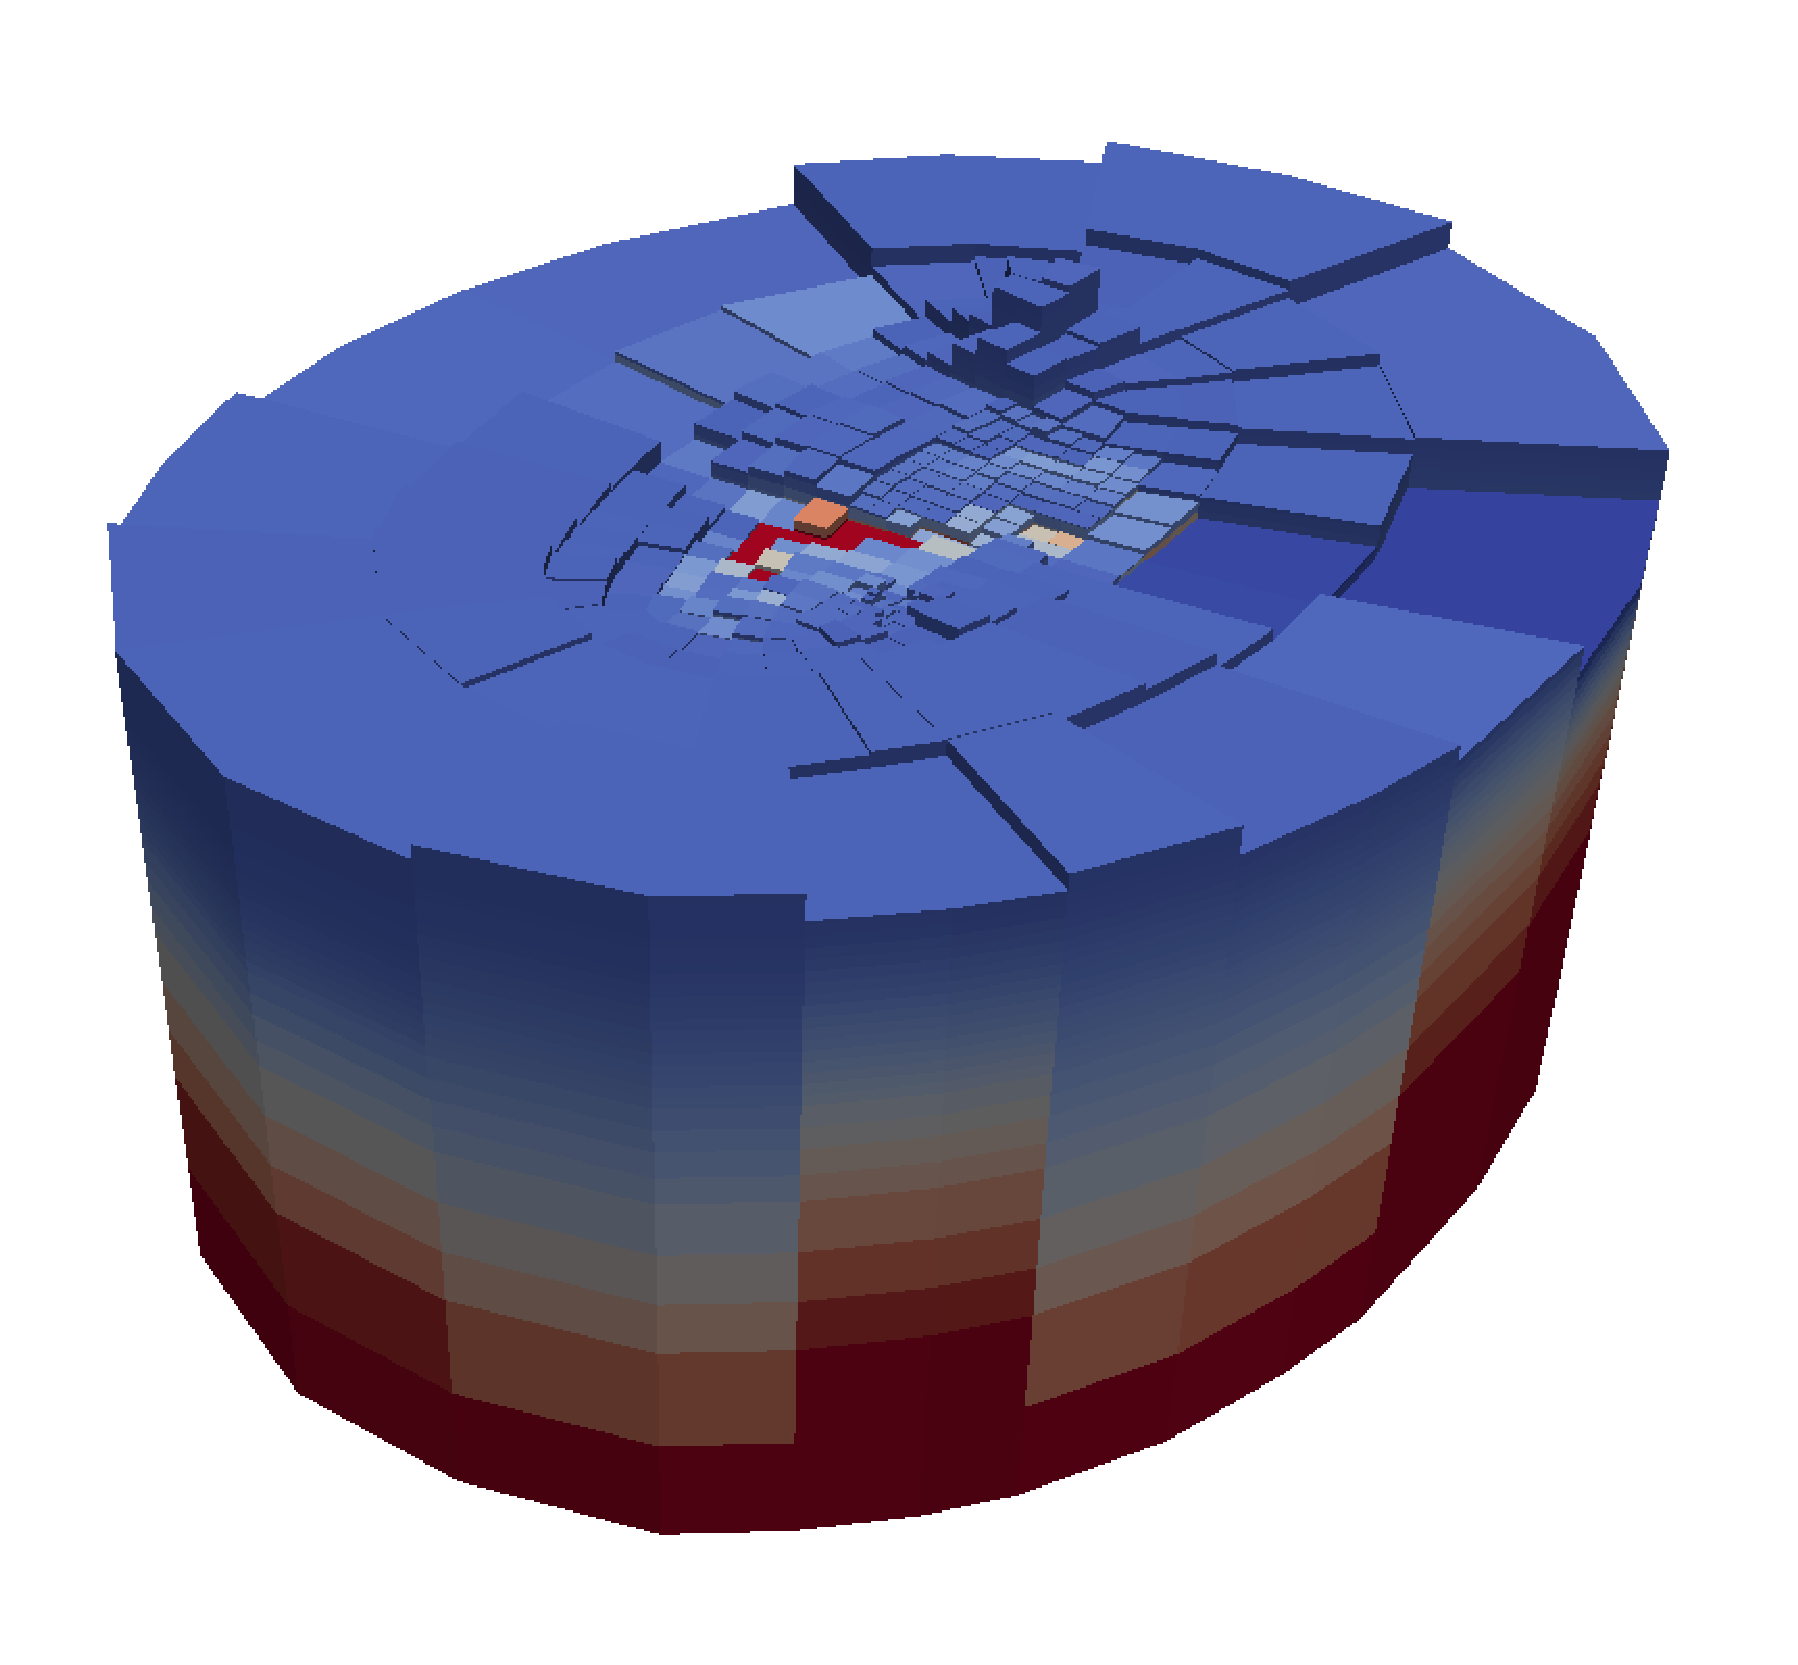
\includegraphics[width=0.75\textwidth]{coverpic}

\bigskip

\textbf{\large{Dr. Adrian Croucher\\
Department of Engineering Science\\
University of Auckland\\
Auckland, New Zealand}}

\bigskip

\textbf{\large{Version 1.3\\
September 2012}}

\bigskip
\bigskip
\bigskip
\bigskip
\bigskip

\includegraphics[width=0.25\textwidth]{UoALogosvg}

\end{center}
\end{titlepage}



%------------------------------------------------------------------------
\tableofcontents
%\listoffigures
\listoftables

%------------------------------------------------------------------------
\chapter{Introduction}

\section{What is PyTOUGH?}

PyTOUGH (\textbf{Py}thon \textbf{TOUGH}) is a set of Python software routines for making it easier to use the TOUGH2 geothermal reservoir simulator. Using PyTOUGH, it is possible to automate the creation and editing of TOUGH2 model grids and data files, and the analysis and display of model simulation results.

\section{What are TOUGH2 and AUTOUGH2?}

TOUGH2 \citep{tough2} is a general-purpose simulator for modelling subsurface fluid and heat flow, often used for simulating geothermal reservoirs.

AUTOUGH2 is the University of Auckland version of TOUGH2.  The main differences between AUTOUGH2 and TOUGH2 are:

\begin{itemize}
  \item \textbf{EOS handling}: AUTOUGH2 includes all different equations of state (EOSes) in a single executable program, whereas TOUGH2 uses different executables for each EOS.  As a result, the main input data file for an AUTOUGH2 simulation also includes extra data blocks to specify which EOS is to be used.
  \item \textbf{Generator types}: AUTOUGH2 includes a variety of extra generator types developed for geothermal reservoir simulation (e.g. makeup and reinjection wells).
\end{itemize}

TOUGH2\_MP \citep{tough2mp} is a multi-processor version of TOUGH2.  TOUGH+ is a redeveloped version of TOUGH2, with a more modular code structure implemented in Fortran-95.

\subsection{TOUGH2 data files}

TOUGH2 takes its main input from a \textbf{data file}, which contains information about the model grid, simulation parameters, time stepping, sources of heat and mass etc.  The data file formats for TOUGH2 and AUTOUGH2 are almost identical, with minor differences.  TOUGH2\_MP can read TOUGH2 data files, but also supports some extensions (e.g. for 8-character instead of 5-character block names) to this format.  PyTOUGH does not currently support the TOUGH2\_MP extensions.  TOUGH+ data files can also have some extensions, which PyTOUGH does not support as yet.

Because TOUGH2 uses a finite volume formulation, the only model grid data it needs are the volumes of the grid blocks and the distances and areas associated with the connections between blocks.  Hence, the TOUGH2 data file need not contain any information about the specific locations of the blocks in space, and it contains no information about the locations of the vertices or edges of the blocks.  This makes it easy to use TOUGH2 to simulate one-, two- or three-dimensional models, all with the same format of data file.  However, this lack of reference to any coordinate system also makes it more difficult to generate model grids, and to visualise simulation results in space.

\subsection{MULgraph geometry files}

For this reason, a separate \textbf{geometry file} can be used to create grids for TOUGH2 simulations and visualise simulation results.  The geometry file contains information about the locations of the grid block vertices.  The geometry file can be used to visualise results using the \textbf{MULgraph} graphical post-processor for TOUGH2 and AUTOUGH2 \citep{mulgraph}, developed at the University of Auckland in the 1990s.

The MULgraph geometry file assumes the grid has a layered structure, with blocks arranged in layers and columns, and the same arrangement of columns on each layer.  (At the top of the model grid, blocks in some columns may be missing, to allow the grid to follow the surface topography.)

\subsection{TOUGH2 listing files}

The output from TOUGH2 is written to a \textbf{listing file}, which is a text file containing tables of results for each time step (or only selected time steps, if preferred).  At each time step there is an `element table', containing results for block properties (e.g. pressure, temperature etc.).  There may also be a `connection table', containing results for flows between blocks, and a `generation table', containing results (e.g. flow rates) at the generators in the model (e.g. wells).

The formats of the listing files produced by TOUGH2, AUTOUGH2, TOUGH2\_MP and TOUGH+ are all slightly different, and also vary depending on the EOS used.  However, PyTOUGH attempts to detect and read all of these formats.

\section{What is Python?}

Python is a general-purpose programming language.  It is free and open-source, and runs on many different computer operating systems (Linux, Windows, Mac OS X and others).  Python can be downloaded from the Python website (\url{http://www.python.org}), which also contains detailed reference material about the Python language.  If you are using Linux you probably already have Python, as it is included in most Linux distributions.

PyTOUGH should run on any version of Python 2.x newer than 2.4 (though version 2.5 or newer is recommended).  Currently PyTOUGH will not run on Python 3.x (which is not backwards compatible with the 2.x series).

If you are unfamiliar with Python (even if you have used another programming language before), it is highly recommended that you do one of the many Python tutorials available online, e.g.

\begin{itemize}
  \item \url{http://docs.python.org/tutorial/}
  \item \url{http://wiki.python.org/moin/BeginnersGuide}
\end{itemize}

\subsection{Python basics}

\subsubsection{Objects}

Python is what is known as an \textbf{object-oriented} language, which means that it is possible to create special customised data types, or `classes', to encapsulate all the properties and behaviour of the things (objects) we are dealing with in a program.  This is a very useful way of simplifying complex programs.  (In fact, in Python, everything is treated as an object, even simple things like integers and strings.)

For example, in a TOUGH2 model grid we have collections of grid blocks, and we need to store the names of these blocks and their volumes and rock types.  In a non-object-oriented language, these could be stored in three separate arrays: a string array for the names, a real (or `float') array for the volumes and another string array for the rock types.  In an object-oriented language like Python, we can define a new data type (or `class') for blocks, which holds the name, volume and rock type of the block.  If we declare an object called \texttt{blk} of this block class, we can access or edit its volume by referring to \texttt{blk.volume}.  In this way, we can store our blocks in one single array of block objects.  When we add or delete blocks from our grid, we can just add or delete block objects from the array, rather than having to keep track of three separate arrays.

In general, an object not only has \textbf{properties} (like \texttt{blk.volume}) but also \textbf{methods}, which are functions the object can carry out.  For example, if we wanted to rotate a MULgraph geometry file by $30\degree$, we could do this in PyTOUGH by declaring a MULgraph geometry file object called \texttt{geo}, and calling its \texttt{rotate} method: \texttt{geo.rotate(30)}.  The methods of an object are accessed in the same way that its properties are accessed: by adding a dot (.) after the object's name and then adding the name of the property or method.  Any arguments of the method (e.g. the angle in the \texttt{rotate} function above) are added in parentheses afterwards.

\subsubsection{Lists, dictionaries, tuples and sets}

Most programming languages have simple data types built in, e.g. float, double precision or integer numbers, strings, and arrays of these.  Python has some other data types which are very useful and are used a lot.

The first of these is the \textbf{list}.  A list can contain any ordered collection of objects, of any type, or even of different types, and is delimited by square brackets.  So for example we can declare a list \texttt{things = [1,`two',3.0]} containing an integer, a string and a float.  We can access the list's elements in much the same way as we access the elements of an array, for example \texttt{things[1]} would return the value \texttt{`two'} (note that in Python, as in most other languages besides Fortran, the indices of arrays and lists start at 0, not 1).  Additional elements can be added to a list at any time, without having to re-declare the size of the list: for example, \texttt{things.append(`IV')} would add an extra element to the end of the list, giving it the value \texttt{[1,`two',3.0,`IV']}.  It is also possible to remove elements from a list, e.g. \texttt{things.remove(3.0)}, which would give our list the value \texttt{[1,`two',`IV']}.

Another useful Python data type is the \textbf{dictionary}.  Dictionaries are mainly used to store collections of objects (again, of any type or of different types) that are referenced by name rather than by index (as in an array or list).  A dictionary is delimited by curly brackets.  So for example we can declare a dictionary \texttt{phone=\{`Eric':8155,`Fred':2350,`Wilma':4667\}} and then find Fred's phone number from \texttt{phone[`Fred']}, which would return \texttt{2350}.  For TOUGH2 models, blocks, generators, rock types and other objects are often referred to by name rather than index, so dictionaries are an appropriate way to store them.

A third Python data type, similar to a list, is the \textbf{tuple}.  A tuple is essentially a list that cannot be changed, and is often used just for grouping objects together.  A tuple is delimited by parentheses.  For example, \texttt{things=(1,`two',3.0)} declares a tuple with three elements.  We can still refer to the elements of a tuple using e.g. \texttt{a[1]}, but we cannot assign new values to these elements or add or remove elements from the tuple once it has been declared.

Python also has a \textbf{set} data type, which represents a mathematical set- an unordered collection of objects.  One of the useful aspects of sets is that they cannot contain duplicate items.  As a result, for example, duplicate items can be removed from a list \texttt{x} simply by converting it to a set, and then back to a list: \texttt{x=list(set(x))}.

\subsection{How to run Python}

Python can be run either interactively or via scripts.

\subsubsection{Running Python interactively}
\label{python_interactive}

The simplest way to run Python interactively is just by typing \texttt{python} at the command line.  (On Windows the directory that Python was installed into may have to be added to your \texttt{PATH} environment variable first.) The command line then becomes an interactive Python environment in which you can type Python commands at the Python command prompt \texttt{>>>}, e.g. in Windows:

\begin{verbatim}
C:\>python
Python 2.6.4 (r264:75708, Oct 26 2009, 08:23:19) [MSC v.1500 32 bit (Intel)]
on win32
Type "help", "copyright", "credits" or "license" for more information.
>>> things = [1,`two',3.0]
>>> print things[1]
two
>>> exit()

C:\>
\end{verbatim}

In the interactive Python environment, you can view help on the properties and methods of any Python object by typing \texttt{help(\emph{objectname})}, where \texttt{\emph{objectname}} is the name of an object that has been declared.  This will list the properties and methods of the object and a description of each one.

You can exit the interactive Python environment by typing \texttt{exit()} or \texttt{Ctrl-Z} on Windows, or \texttt{Ctrl-D} on Linux.

\subsubsection{Python scripts}

The real power of Python, however, lies in using it to write \textbf{scripts} to automate repetitive or complex tasks.  You can just type Python commands into a text file, save it with the file extension \texttt{.py}, and execute it by typing \texttt{python \emph{filename.py}}, where \texttt{\emph{filename.py}} is the name of the file.  (Once again, on Windows the directory that Python was installed into may have to be added to your \texttt{PATH} environment variable first.)

You can also debug a Python script using the `pdb' command-line debugger.  Typing \texttt{python -m pdb \emph{filename.py}} will start debugging the script \emph{filename.py}.

It is also possible to run a Python script from within the interactive Python environment.  From the Python environment command line, typing \texttt{execfile(\emph{`filename.py'})} will execute the script \emph{filename.py}.

\subsection{Python libraries}
\label{pylibraries}

Python comes with a large number of features already built in, but for specialised tasks, additional \textbf{libraries} of Python software can be imported into Python as you need them.  PyTOUGH itself is a set of such libraries, and it in turn makes use of some other Python libraries.

\subsubsection{Numerical Python}

The most important of these is Numerical Python (`numpy'), which you will need to have installed on your computer before you can use PyTOUGH at all \footnote{PyTOUGH will run using Numeric, a now-obsolete predecessor of Numerical Python, though the PyTOUGH plotting functions will not work.  In general it is recommended to use Numerical Python if possible.}.  Numerical Python adds a special \texttt{numpy.array} class for fast multi-dimensional arrays, which PyTOUGH makes heavy use of, and a whole range of other features, e.g. linear algebra routines, Fourier transforms and statistics.

Numerical Python can be freely downloaded from \url{http://numpy.scipy.org/} (or simply installed via your package manager on Linux). The latest versions may not yet be available for 64-bit Windows from this site.  However, you can find unofficial builds at \texttt{http://www.lfd.uci.edu/\textasciitilde gohlke/pythonlibs/}.

\subsubsection{Other libraries}

Some parts of PyTOUGH use other Python libraries.  You do not need these libraries unless you are using the parts of PyTOUGH that depend on them.

\begin{itemize}
\item \textbf{matplotlib} (\url{http://matplotlib.sourceforge.net/}), a library of graphical plotting routines
\item \textbf{Scientific Python} (\url{http://www.scipy.org/}), a library of advanced mathematical functions (e.g. interpolation, calculus, optimisation)
\item \textbf{VTK} (\url{http://www.vtk.org/}), the Visualization Tool Kit (a library for 3D visualisation of data via VTK itself, or software such as ParaView, Mayavi etc.) and \textbf{VTK Python}, the Python interface for VTK.
\end{itemize}

On Linux systems you can download and install these libraries via your package manager (e.g. on Debian or Debian-based distributions like Ubuntu, \texttt{aptitude install python-matplotlib python-scipy libvtk5.4 python-vtk}).

On Windows you will need to download and install them yourself from the internet (see links above) or elsewhere.  At the time of writing there is not yet an official 64-bit build of Scientific Python for Windows.  However an unofficial build can be found at \url{http://www.lfd.uci.edu/\textasciitilde gohlke/pythonlibs/}.  Use of this version of Scientific Python requires that their version of Numerical Python is also used.

\subsubsection{Installing VTK-Python on Windows}

There does not appear to be an official Windows build of VTK Python, but you can instead download an unofficial Python-enabled Windows version of VTK (i.e. VTK with VTK Python included) from \url{http://www.lfd.uci.edu/\textasciitilde gohlke/pythonlibs/}.

Make sure you download and install the right version, corresponding to the version of Python you are using.  You will need to add a few things to the environment variables on your system to get it to work.  (If you aren't sure how to edit your environment variables, see section \ref{installing} below.) 

In the directory where VTK is installed to, there should be sub-directories called something like \texttt{VTK\textbackslash bin} and \texttt{VTK\textbackslash lib\textbackslash site-packages}.  You need to add the full path to the \texttt{bin} directory to the PATH environment variable on your system, and the paths to both the \texttt{bin} and \texttt{lib\textbackslash site-packages} directories to your PYTHONPATH environment variable.

Alternatively, there are third-party repackaged distributions of Python which come bundled with some or all of these additional libraries (see \url{http://www.python.org/download/}).

\subsubsection{Importing libraries}

To use any Python library, you just need to \textbf{import} it first.  For example, once you have installed Numerical Python, you can make it available (in the interactive Python environment or in a Python script) by typing the command \texttt{import numpy}, or alternatively \texttt{from numpy import *}.  This imports all classes and commands from Numerical Python and makes them available for use.  (You can also import only parts of a library rather than the whole thing, e.g. \texttt{from numpy import linalg} just imports the linear algebra routines from Numerical Python.)

When you import a library, you can also change its name.  For example, PyTOUGH imports Numerical Python using the command \texttt{import numpy as np}, which renames \texttt{numpy} as the abbreviated \texttt{np}.  This means it can, for example, access the Numerical Python \texttt{numpy.array} data type as \texttt{np.array}.  It also means you have access to Numerical Python as \texttt{np} in your own scripts and in the interactive Python environment, without having to import it yourself.

\section{Installing and accessing PyTOUGH}
\label{installing}

First, make sure you have Python, and the Numerical Python library (see section \ref{pylibraries}) installed.  On Windows, you may have to add the directory where Python has installed (e.g. \texttt{C:\textbackslash Python26} or similar, depending on which version you have) to your PATH environment variable, before you can access Python from the command line.

On the PyTOUGH website, click the `Download ZIP' button at the right of the page:

\url{https://github.com/acroucher/PyTOUGH/archive/master.zip}

to download PyTOUGH as a .zip file.  Unzip this to any directory on your computer.  This will create a directory containing a file called \texttt{setup.py}.

To install PyTOUGH, you will need administrator (`root' on Linux) privileges on your computer.  As administrator, open a command prompt, navigate to this new directory and type:

\begin{verbatim}
python setup.py install
\end{verbatim}

You should now be able to import the PyTOUGH libraries into the Python interactive environment or your Python scripts, from any directory on your computer.  For example, you can import the MULgraph geometry library using \texttt{from mulgrids import *} (see chapter \ref{mulgrids}).

\section{Licensing}

PyTOUGH is free software, distributed under the GNU Lesser General Public License (LGPL).  For more information, see \url{http://www.gnu.org/licenses/}.

\chapter{MULgraph geometry files}
\label{mulgrids}

\section{Introduction}
The \texttt{mulgrids} library in PyTOUGH contains classes and routines for creating, editing and saving MULgraph geometry files.  It can be imported using the command:

\begin{lstlisting}
  from mulgrids import *
\end{lstlisting}

\section{\texttt{mulgrid} objects}
\index{MULgraph geometry!objects}
\index{MULgraph geometry!creating}
\index{PyTOUGH!classes!\texttt{mulgrid}}

The \texttt{mulgrids} library defines a \texttt{mulgrid} class, used for representing MULgraph geometry files.

\textbf{Example:}

\begin{lstlisting}
geo = mulgrid()
\end{lstlisting}

creates an empty \texttt{mulgrid} object called \texttt{geo}.

\begin{lstlisting}
geo = mulgrid('geom.dat')
\end{lstlisting}

creates a \texttt{mulgrid} object called \texttt{geo} and reads its contents from a file named \texttt{'geom.dat'}.

Printing a \texttt{mulgrid} object (e.g. \texttt{print geo}) displays a summary of information about the grid: how many nodes, columns, layers, blocks and wells it contains, as well as its naming convention and atmosphere type.

A specification of the MULgraph geometry file format can be found in Appendix \ref{geometry_file_format}.

\subsection{Properties}
\index{MULgraph geometry!properties}

The main properties of a \texttt{mulgrid} object are listed in Table \ref{tb:mulgrid_properties}.  Some of these properties are `header' information, corresponding to the data at the start of a MULgraph geometry file (\texttt{type}, \texttt{convention}, \texttt{atmosphere\_type}, \texttt{atmosphere\_volume}, \texttt{atmosphere\_connection} and \texttt{unit\_type}).

The most important properties of a \texttt{mulgrid} object are \texttt{node}, \texttt{column}, \texttt{connection}, \texttt{layer} and \texttt{well}, which are dictionaries of the grid nodes, columns, connections, layers and wells, accessed by name.  For example, grid layer `AA' of a \texttt{mulgrid} object \texttt{geo} can be accessed by \texttt{geo.layer['AA']}.  (The \texttt{nodelist}, \texttt{columnlist}, \texttt{connectionlist}, \texttt{layerlist} and \texttt{welllist} properties offer access to the nodes, columns, connections, layers and wells by index, which is sometimes useful e.g. for looping over all columns in the grid.)

Connections are slightly different from nodes, columns etc. in that they are not named individually.  However, they can be accessed by the names of the columns connected by the connection.  For example, the connection between columns ` 10' and ` 11' in a \texttt{mulgrid} called \texttt{geo} is given by \texttt{geo.connection[' 10',' 11']}.

The elements of these lists and dictionaries are of type \texttt{node}, \texttt{column}, \texttt{connection}, \texttt{layer} and \texttt{well} respectively.  These are additional object classes to represent nodes, columns, connections, layers and wells, defined in the \texttt{mulgrids} library (see section \ref{other_mulgrid_objects}).

\subsubsection{Grid diagnostics}
\index{MULgraph geometry!diagnostics}

A \texttt{mulgrid} object has some properties (and methods) for evaluating its integrity.  The property \texttt{column\_angle\_ratio} returns an \texttt{np.array} of the `angle ratio' for each column (the ratio of largest to smallest interior angles - see section \ref{columnobjects}), a measure of skewness.  The \texttt{column\_side\_ratio} returns an \texttt{np.array} of the `side ratio' for each column (the ratio of largest to smallest side length), a measure of elongation.  These array properties can be plotted using the \texttt{layer\_plot} method (see section \ref{mulgridmethods}) for a graphical overview of grid quality.

There is also a \texttt{connection\_angle\_cosine} property, which returns an \texttt{np.array} of the angle cosine for each connection (the cosine of the angle between a line joining the nodes in the connection and a line joining the centres of the blocks in the connection).  In general it is desirable for these lines to be as close to perpendicular as possible, making the cosines close to zero.

The \texttt{bad\_columns}, \texttt{bad\_layers}, \texttt{missing\_connections}, \texttt{extra\_connections} and \texttt{orphans} properties return actual problems with the grid which should be fixed.  A summary of all these problems is given by the \texttt{check} method (see section \ref{mulgridmethods}).

Blocks at the ground surface that have very small vertical thickness can sometimes cause problems.  The \texttt{min\_surface\_block\_thickness} property gives a tuple containing the minimum surface block thickness and the name of the column in which it occurs.  Thin surface blocks of this type can be eliminated using the \texttt{snap\_columns\_to\_layers()} method.

\subsubsection{Functions for reading data from file}
\label{mulgridreadfunctions}
\index{MULgraph geometry!file format}
\index{MULgraph geometry!reading}

A \texttt{mulgrid} object has a \texttt{read\_function} property which controls how data are read from file.  This property is a dictionary with six keys: `d', `f', `e', `g', `s' and `x', denoting respectively integer, float, exponential, general, string and blank.  Each item in the dictionary is a function which converts a string from the file on disk into the appropriate value.  For example, \texttt{read\_function['f']} converts a string to a floating point value.  By default, the built-in Python \texttt{float} function is used for this (although it is modified slightly so that it returns \texttt{None} if the input string is blank).  There is a dictionary of default reading functions included in PyTOUGH, called \texttt{default\_read\_function}.

However, the user can specify other functions if needed.  In particular, files produced from Fortran programs sometimes have formatting that is not readable by the default functions, if some more exotic Fortran formatting options have been used.   For example, a `d' can also be used to represent an exponent (like `e'), or spaces can be included within a number, or the exponent identifier (e.g. `e') can be omitted.  PyTOUGH includes a second set of reading functions, called \texttt{fortran\_read\_function}, for handling Fortran formatting.  These are slightly slower than the default reading functions.

The reading functions for a \texttt{mulgrid} object can be specified when the object is being created, e.g.:

\begin{lstlisting}
geo = mulgrid('geom.dat', read_function = fortran_read_function)
\end{lstlisting}

\subsubsection{Tilted geometries}
\index{MULgraph geometry!tilting}

Non-horizontal (i.e. tilted) geometries can be constructed by setting the \texttt{mulgrid} properties \texttt{gdcx} and \texttt{gdcy} non-zero. These properties represent the cosines of the angles the x- and y-axes make with the gravity vector. By default they are both zero, giving a horizontal grid. A geometry with \texttt{gdcx} = 1 can be used to construct a 2-D vertical slice grid with a non-layered structure. When a \texttt{t2grid} object is created from a tilted geometry, e.g. using the \texttt{t2grid} \hyperref[sec:t2grid:fromgeo]{fromgeo()} method, only the gravity cosines of the connections are affected (the \texttt{dircos} property of each connection).

\subsubsection{Rotating permeability directions}
\index{MULgraph geometry!permeability directions}

It is possible to rotate the permeability principal directions of a \texttt{mulgrid} object with respect to the coordinate axes- for example, to align permeabilities with a dominant fault direction- by specifying the \texttt{permeability\_angle} property. When a \texttt{t2grid} object is created, e.g. using the \texttt{t2grid} \hyperref[sec:t2grid:fromgeo]{fromgeo()} method, this can change the \texttt{direction} property of each connection.

\index{MULgraph geometry!properties}
\begin{center}
  \begin{longtable}{|l|l|p{75mm}|}
    \hline
    \textbf{Property} & \textbf{Type} & \textbf{Description}\\
    \hline
    \texttt{area} & float & total horizontal area covered by the grid \\
    \texttt{atmosphere\_connection} & float & connection distance to atmosphere blocks\\
    \texttt{atmosphere\_type} & integer & type of atmosphere\\
    \texttt{atmosphere\_volume} & float & volume of atmosphere blocks\\
    \texttt{bad\_columns} & set & columns that do not contain their own centres\\
    \texttt{bad\_layers} & set & layers that do not contain their own centres\\
    \texttt{block\_connection\_name\_index} & dictionary & indices of block connections (by name)\\
    \texttt{block\_connection\_name\_list} & list & names of block connections (by index)\\
    \texttt{block\_name\_index} & dictionary & indices of blocks (by name)\\
    \texttt{block\_name\_list} & list & names of blocks (by index)\\
    \texttt{boundary\_columns} & set & set of columns on the outer boundary of the grid \\
    \texttt{boundary\_nodes} & list & ordered list of nodes on the outer boundary of the grid \\
    \texttt{boundary\_polygon} & list & list of points representing grid boundary (extra colinear points removed) \\
    \texttt{bounds} & list & [bottom left, top right] horizontal bounds of grid\\
    \texttt{centre} & \texttt{np.array} & position of horizontal centre of the grid \\
    \texttt{columnlist} & list & columns (by index, e.g. \texttt{columnlist[23]})\\
    \texttt{column\_angle\_ratio} & \texttt{np.array} & angle ratio for each column\\
    \texttt{column\_side\_ratio} & \texttt{np.array} & side ratio for each column\\
    \texttt{column} & dictionary & columns (by name, e.g. \texttt{column['AA']})\\
    \texttt{connection\_list} & list & connections between columns (by index)\\
    \texttt{connection\_angle\_cosine} & \texttt{np.array} & angle cosines for all connections\\
    \texttt{convention} & integer & naming convention for columns and layers\\
    \texttt{default\_surface} & Boolean  & \texttt{True} if all columns have default surface elevation\\
    \texttt{extra\_connections} & set & connections defined between columns that are not against each other\\
    \texttt{filename} & string  & file name on disk\\
    \texttt{gdcx}, \texttt{gdcy} & float  & cosines of angles x- and y-axes make with gravity vector\\
    \texttt{node\_kdtree} & \texttt{cKDTree} & tree structure for fast searching for nodes \\
    \texttt{layerlist} & list & layers (by index)\\
    \texttt{layer} & dictionary & layers (by name)\\
    \texttt{min\_surface\_block\_thickness} & (float, string) & thickness of thinnest surface block (and associated column name)\\
    \texttt{missing\_connections} & set & missing connections between columns\\
    \texttt{nodelist} & list  & nodes (by index)\\
    \texttt{node} & dictionary  & nodes (by name)\\
    \texttt{num\_atmosphere\_blocks} & integer & number of atmosphere blocks\\
    \texttt{num\_blocks} & integer & total number of blocks in the grid\\
    \texttt{num\_block\_connections} & integer & total number of block connections in the grid\\
    \texttt{num\_columns} & integer & number of columns\\
    \texttt{num\_connections} & integer & number of connections between columns\\
    \texttt{num\_layers} & integer & number of layers\\
    \texttt{num\_nodes} & integer & number of nodes\\
    \texttt{num\_underground\_blocks} & integer & number of non-atmosphere blocks\\
    \texttt{num\_wells} & integer & number of wells\\
    \texttt{orphans} & set & orphaned nodes (nodes not belonging to any column)\\
    \texttt{permeability\_angle} & float & rotation angle (degrees anticlockwise) of first horizontal permeability direction \\
    \texttt{read\_function} & dictionary & dictionary of functions used to read data from file\\
    \texttt{type} & string  & type of geometry (currently only `GENER' supported)\\
    \texttt{unit\_type} & string & distance unit (blank for metres, `FEET' for ft)\\
    \texttt{welllist} & list & wells (by index)\\
    \texttt{well} & dictionary & wells (by name)\\
    \hline
    \caption{Properties of a \texttt{mulgrid} object}
    \label{tb:mulgrid_properties}
  \end{longtable}
\end{center}

\subsection{Methods}
\label{mulgridmethods}

The main methods of a \texttt{mulgrid} object are listed in Table \ref{tb:mulgrid_methods}.  Details of these methods are given below.

\index{MULgraph geometry!methods}
\begin{center}
\begin{longtable}{|l|l|p{70mm}|}
  \hline
  \textbf{Method} & \textbf{Type} & \textbf{Description}\\
  \hline
  \hyperref[sec:mulgrid:add_column]{\texttt{add\_column}} & -- & adds a column to the grid\\ 
  \hyperref[sec:mulgrid:add_connection]{\texttt{add\_connection}} & -- & adds a connection to the grid\\ 
  \hyperref[sec:mulgrid:add_layer]{\texttt{add\_layer}} & -- & adds a layer to the grid\\ 
  \hyperref[sec:mulgrid:add_node]{\texttt{add\_node}} & -- & adds a node to the grid\\ 
  \hyperref[sec:mulgrid:add_well]{\texttt{add\_well}} & -- & adds a well to the grid\\ 
  \hyperref[sec:mulgrid:block_centre]{\texttt{block\_centre}} & \texttt{np.array} & block centre\\
  \hyperref[sec:mulgrid:block_contains_point]{\texttt{block\_contains\_point}} & Boolean & whether a block contains a 3D point\\
  \hyperref[sec:mulgrid:block_mapping]{\texttt{block\_mapping}} & dictionary & mapping from the blocks of another \texttt{mulgrid} object\\
  \hyperref[sec:mulgrid:block_name]{\texttt{block\_name}} & string & name of block at given layer and column\\
  \hyperref[sec:mulgrid:block_name_containing_point]{\texttt{block\_name\_containing\_point}} & string & name of block containing specified point\\
  \hyperref[sec:mulgrid:block_surface]{\texttt{block\_surface}} & float & block top elevation\\
  \hyperref[sec:mulgrid:block_volume]{\texttt{block\_volume}} & float & block volume\\
  \hyperref[sec:mulgrid:check]{\texttt{check}} & Boolean & checks grid for errors (and optionally fixes them)\\ 
  \hyperref[sec:mulgrid:column_boundary_nodes]{\texttt{column\_boundary\_nodes}} & list & nodes around the outer boundary of a group of columns\\ 
  \hyperref[sec:mulgrid:column_bounds]{\texttt{column\_bounds}} & list & bounding rectangle around a list of columns\\ 
  \hyperref[sec:mulgrid:column_containing_point]{\texttt{column\_containing\_point}} & column & column containing specified horizontal point\\ 
  \hyperref[sec:mulgrid:column_mapping]{\texttt{column\_mapping}} & dictionary & mapping from the columns of another \texttt{mulgrid} object\\
  \hyperref[sec:mulgrid:column_name]{\texttt{column\_name}} & string & column name of a block name\\ 
  \hyperref[sec:mulgrid:column_neighbour_groups]{\texttt{column\_neighbour\_groups}} & list & groups connected columns\\ 
  \hyperref[sec:mulgrid:column_quadtree]{\texttt{column\_quadtree}} & quadtree & quadtree structure for searching columns\\ 
  \hyperref[sec:mulgrid:column_surface_layer]{\texttt{column\_surface\_layer}} & \hyperref[layerobjects]{\texttt{layer}} & surface layer for a specified column\\
  \hyperref[sec:mulgrid:column_values]{\texttt{column\_values}} & tuple & values of a variable down a column\\
  \hyperref[sec:mulgrid:columns_in_polygon]{\texttt{columns\_in\_polygon}} & list & columns inside a specified polygon (or rectangle)\\ 
  \hyperref[sec:mulgrid:connects]{\texttt{connects}} & Boolean & whether the grid has a connection between two specified columns\\ 
  \hyperref[sec:mulgrid:copy_layers_from]{\texttt{copy\_layers\_from}} & -- & copies layer structure from another geometry\\ 
  \hyperref[sec:mulgrid:copy_wells_from]{\texttt{copy\_wells\_from}} & -- & copies wells from another geometry\\ 
  \hyperref[sec:mulgrid:decompose_columns]{\texttt{decompose\_columns}} & -- & decomposes columns into triangles and quadrilaterals\\ 
  \hyperref[sec:mulgrid:delete_column]{\texttt{delete\_column}} & -- & deletes a column from the grid\\ 
  \hyperref[sec:mulgrid:delete_connection]{\texttt{delete\_connection}} & -- & deletes a connection from the grid\\ 
  \hyperref[sec:mulgrid:delete_layer]{\texttt{delete\_layer}} & -- & deletes a layer from the grid\\ 
  \hyperref[sec:mulgrid:delete_node]{\texttt{delete\_node}} & -- & deletes a node from the grid\\ 
  \hyperref[sec:mulgrid:delete_orphans]{\texttt{delete\_orphans}} & -- & deletes any orphaned nodes from the grid\\ 
  \hyperref[sec:mulgrid:delete_orphan_wells]{\texttt{delete\_orphan\_wells}} & -- & deletes any orphaned wells from the grid\\ 
  \hyperref[sec:mulgrid:delete_well]{\texttt{delete\_well}} & -- & deletes a well from the grid\\ 
  \hyperref[sec:mulgrid:empty]{\texttt{empty}} & --  & empties contents of grid\\
  \hyperref[sec:mulgrid:export_surfer]{\texttt{export\_surfer}} & -- & exports to various files on disk for visualization in Surfer\\ 
  \hyperref[sec:mulgrid:fit_columns]{\texttt{fit\_columns}} & \texttt{np.array} or dictionary & fits scattered data to column centres\\ 
  \hyperref[sec:mulgrid:fit_surface]{\texttt{fit\_surface}} & -- & fits column surface elevations from data\\ 
  \hyperref[sec:mulgrid:from_gmsh]{\texttt{from\_gmsh}} & \hyperref[mulgrids]{\texttt{mulgrid}} & imports a grid from a \texttt{gmsh} mesh\\ 
  \hyperref[sec:mulgrid:layer_containing_elevation]{\texttt{layer\_containing\_elevation}} & layer & layer containing specified vertical elevation\\
  \hyperref[sec:mulgrid:layer_mapping]{\texttt{layer\_mapping}} & dictionary & mapping from the layers of another \texttt{mulgrid} object\\
  \hyperref[sec:mulgrid:layer_name]{\texttt{layer\_name}} & string & layer name of a block name\\ 
  \hyperref[sec:mulgrid:layer_plot]{\texttt{layer\_plot}} & -- & plots a variable over a layer of the grid\\
  \hyperref[sec:mulgrid:line_plot]{\texttt{line\_plot}} & -- & plots a variable along an arbitrary line through the grid\\
  \hyperref[sec:mulgrid:line_values]{\texttt{line\_values}} & tuple & values of a variable along an arbitrary line through the grid\\
  \hyperref[sec:mulgrid:meshio_grid]{\texttt{meshio\_grid}} & tuple & mesh in \texttt{meshio} format\\ 
  \hyperref[sec:mulgrid:minc_array]{\texttt{minc\_array}} & array & values for a particular level in a MINC grid\\ 
  \hyperref[sec:mulgrid:nodes_in_columns]{\texttt{nodes\_in\_columns}} & list & nodes in a specified list of columns\\ 
  \hyperref[sec:mulgrid:nodes_in_polygon]{\texttt{nodes\_in\_polygon}} & list & nodes inside a specified polygon (or rectangle)\\ 
  \hyperref[sec:mulgrid:node_nearest_to]{\texttt{node\_nearest\_to}} & \hyperref[nodeobjects]{\texttt{node}} & node nearest to a specified point\\ 
  \hyperref[sec:mulgrid:optimize]{\texttt{optimize}} & -- & adjusts node positions to optimize grid quality\\
  \hyperref[sec:mulgrid:polyline_values]{\texttt{polyline\_values}} & tuple & values of a variable along an arbitrary polyline through the grid\\
  \hyperref[sec:mulgrid:read]{\texttt{read}} & \hyperref[mulgrids]{\texttt{mulgrid}} & reads geometry file from disk\\
  \hyperref[sec:mulgrid:rectangular]{\texttt{rectangular}} & \hyperref[mulgrids]{\texttt{mulgrid}} & creates rectangular grid\\
  \hyperref[sec:mulgrid:reduce]{\texttt{reduce}} & -- & reduces a grid to contain only specified columns\\
  \hyperref[sec:mulgrid:refine]{\texttt{refine}} & -- & refines specified columns in the grid\\
  \hyperref[sec:mulgrid:refine_layers]{\texttt{refine\_layers}} & -- & refines specified layers in the grid\\
  \hyperref[sec:mulgrid:rename_column]{\texttt{rename\_column}} & Boolean & renames a column\\
  \hyperref[sec:mulgrid:rename_layer]{\texttt{rename\_layer}} & Boolean & renames a layer\\
  \hyperref[sec:mulgrid:rotate]{\texttt{rotate}} & -- & rotates a grid in the horizontal plane\\
  \hyperref[sec:mulgrid:slice_plot]{\texttt{slice\_plot}} & -- & plots a variable over a vertical slice through the grid\\
  \hyperref[sec:mulgrid:snap_columns_to_layers]{\texttt{snap\_columns\_to\_layers}} & -- & snaps column surfaces to layer bottoms\\
  \hyperref[sec:mulgrid:split_column]{\texttt{split\_column}} & Boolean & splits a quadrilateral column into two triangles\\ 
  \hyperref[sec:mulgrid:translate]{\texttt{translate}} & -- & moves a grid by simple translation in 3D\\
  \hyperref[sec:mulgrid:well_values]{\texttt{well\_values}} & tuple & values of a variable down a well\\
  \hyperref[sec:mulgrid:write]{\texttt{write}} & -- & writes to geometry file on disk\\
  \hyperref[sec:mulgrid:write_bna]{\texttt{write\_bna}} & -- & writes to Atlas BNA file on disk\\ 
  \hyperref[sec:mulgrid:write_exodusii]{\texttt{write\_exodusii}} &  -- & writes to ExodusII file on disk\\
  \hyperref[sec:mulgrid:write_mesh]{\texttt{write\_mesh}} &  -- & writes to mesh file (various formats) on disk\\
  \hyperref[sec:mulgrid:write_vtk]{\texttt{write\_vtk}} &  -- & writes to VTK file on disk\\
  \hline
  \caption{Methods of a \texttt{mulgrid} object}
  \label{tb:mulgrid_methods}
\end{longtable}
\end{center}

\begin{snugshade}\subsubsection{\texttt{add\_column(\emph{col})}}\end{snugshade}
\label{sec:mulgrid:add_column}
\index{MULgraph geometry!adding!columns}
\index{MULgraph geometry!columns!adding}

Adds a \hyperref[columnobjects]{\texttt{column}} object \texttt{col}
to the grid. If a column with the same name already exists, no new
column is added.

\begin{snugshade}\subsubsection{\texttt{add\_connection(\emph{con})}}\end{snugshade}
\label{sec:mulgrid:add_connection}
\index{MULgraph geometry!adding!connections}
\index{MULgraph geometry!connections!adding}

Adds a \hyperref[connectionobjects]{\texttt{connection}} object
\texttt{con} to the grid. If a connection with the same name already
exists, no new connection is added.

\begin{snugshade}\subsubsection{\texttt{add\_layer(\emph{lay})}}\end{snugshade}
\label{sec:mulgrid:add_layer}
\index{MULgraph geometry!adding!layers}
\index{MULgraph geometry!layers!adding}

Adds a \hyperref[layerobjects]{\texttt{layer}} object \texttt{lay} to
the grid. If a layer with the same name already exists, no new layer
is added.

\begin{snugshade}\subsubsection{\texttt{add\_node(\emph{n})}}\end{snugshade}
\label{sec:mulgrid:add_node}
\index{MULgraph geometry!adding!nodes}
\index{MULgraph geometry!nodes!adding}

Adds a \hyperref[nodeobjects]{\texttt{node}} object \texttt{n} to the
grid. If a node with the same name already exists, no new node is
added.

\begin{snugshade}\subsubsection{\texttt{add\_well(\emph{w})}}\end{snugshade}
\label{sec:mulgrid:add_well}
\index{MULgraph geometry!adding!wells}
\index{MULgraph geometry!wells!adding}

Adds a \hyperref[wellobjects]{\texttt{well}} object \texttt{w} to the
grid. If a well with the same name already exists, no new well is
added.

\begin{snugshade}\subsubsection{\texttt{block\_contains\_point(\emph{blockname}, \emph{pos})}}\end{snugshade}
\label{sec:mulgrid:block_contains_point}
\index{MULgraph geometry!finding!blocks}
\index{MULgraph geometry!blocks!finding}

Returns \texttt{True} if the grid block with the given name contains the 3D point \texttt{pos}.

\textbf{Parameters:}
\begin{itemize}
\item \textbf{blockname}: string\\
  The name of the block.
\item \textbf{pos}: \texttt{np.array}\\
  3-element array representing the 3D point.
\end{itemize}

\begin{snugshade}\subsubsection{\texttt{block\_centre(\emph{lay}, \emph{col})}}\end{snugshade}
\label{sec:mulgrid:block_centre}
\index{MULgraph geometry!blocks!centres}

Returns the centre of the block corresponding to the given layer and column.

The horizontal centre is given by the column centre. The vertical centre is given by the layer centre, except for surface blocks with column surface lower than the layer top, in which case it is the midpoint between the column surface and the layer bottom.  (For surface blocks with column surface higher than the layer top, the vertical centre is still the layer centre, to give a uniform pressure reference.)

\textbf{Parameters:}
\begin{itemize}
\item \textbf{lay}: \hyperref[layerobjects]{\texttt{layer}} or string\\
  The specified layer or layer name.
\item \textbf{col}: \hyperref[columnobjects]{\texttt{column}} or string\\
  The specified column or column name.
\end{itemize}

\begin{snugshade}\subsubsection{\texttt{block\_mapping(\emph{geo}, \emph{column\_mapping}=\texttt{False})}}\end{snugshade}
\label{sec:mulgrid:block_mapping}

Returns a dictionary mapping each block name in the \texttt{mulgrid} object \texttt{geo} to the name of the nearest block in the object's own geometry.  Can optionally also return the associated column mapping.

\textbf{Parameters:}
\begin{itemize}
\item \textbf{geo}: \hyperref[mulgrids]{\texttt{mulgrid}}\\
  The \texttt{mulgrid} object to create a block mapping from.
\item \textbf{column\_mapping}: Boolean\\
  If \texttt{True}, the column mapping will also be returned (i.e. the function will return a tuple containing the block mapping and the column mapping).  Default value is \texttt{False}.
\end{itemize}

\begin{snugshade}\subsubsection{\texttt{block\_name(\emph{layer\_name}, \emph{column\_name}, \emph{blockmap} = \{\})}}\end{snugshade}
\label{sec:mulgrid:block_name}
\index{MULgraph geometry!blocks!names}
\index{MULgraph geometry!names!of blocks}

Gives the name of the block corresponding to the specified layer and column names, according to the naming convention of the grid.

An optional block name mapping can be applied.

\textbf{Parameters:}
\begin{itemize}
\item \textbf{layer\_name}, \textbf{column\_name}: string\\
  Name of layer and column (the widths of these strings are determined by the grid's naming convention).
\item \textbf{blockmap}: dictionary\\
  Dictionary mapping the block names in the geometry to another block naming system. This dictionary need not contain entries for all blocks in the geometry- those not included in the mapping will not be altered.
\end{itemize}

\begin{snugshade}\subsubsection{\texttt{block\_name\_containing\_point(\emph{pos}, \emph{qtree}=None, \emph{blockmap}=\{\})}}\end{snugshade}
\label{sec:mulgrid:block_name_containing_point}
\index{MULgraph geometry!finding!blocks}
\index{MULgraph geometry!blocks!finding}
\index{MULgraph geometry!columns!quadtrees}
\index{quadtrees}

Gives the name of the block containing a specified 3-D position in the grid (returns \texttt{None} if the point lies outside the grid).

\textbf{Parameters:}
\begin{itemize}
\item \textbf{pos}: \texttt{np.array}\\
  Position of point in 3-D
\item \textbf{qtree}: \texttt{quadtree}\\
  Quadtree object for fast searching of grid columns (can be constructed using the \hyperref[sec:mulgrid:column_quadtree]{\texttt{column\_quadtree()}} method).
\item \textbf{blockmap}: dictionary\\
  Dictionary mapping the block names in the geometry to another block naming system.
\end{itemize}

\begin{snugshade}\subsubsection{\texttt{block\_surface(\emph{lay}, \emph{col})}}\end{snugshade}
\label{sec:mulgrid:block_surface}
\index{MULgraph geometry!blocks!surfaces}

Returns the elevation of the top surface of the block corresponding to the given layer and column.

\textbf{Parameters:}
\begin{itemize}
\item \textbf{lay}: \hyperref[layerobjects]{\texttt{layer}}\\
  The specified layer.
\item \textbf{col}: \hyperref[columnobjects]{\texttt{column}}\\
  The specified column.
\end{itemize}

\begin{snugshade}\subsubsection{\texttt{block\_volume(\emph{lay}, \emph{col})}}\end{snugshade}
\label{sec:mulgrid:block_volume}
\index{MULgraph geometry!blocks!volumes}

Returns the volume of the block corresponding to the given layer and column.

\textbf{Parameters:}
\begin{itemize}
\item \textbf{lay}: \hyperref[layerobjects]{\texttt{layer}}\\
  The specified layer.
\item \textbf{col}: \hyperref[columnobjects]{\texttt{column}}\\
  The specified column.
\end{itemize}

\begin{snugshade}\subsubsection{\texttt{check(\emph{fix}=False,\emph{silent}=False)}}\end{snugshade}
\label{sec:mulgrid:check}
\index{MULgraph geometry!checking}
\index{checking!MULgraph geometry}

Checks a grid for errors and optionally fixes them.  Errors checked for are: missing connections, extra connections, orphaned nodes, and columns and layers that do not contain their own centres.  Returns \texttt{True} if no errors were found, and \texttt{False} otherwise.  If \texttt{fix} is \texttt{True}, any identified problems will be fixed.  If \texttt{silent} is \texttt{True}, there is no printout (only really useful if \texttt{fix} is \texttt{True}).

\textbf{Parameters:}
\begin{itemize}
\item \textbf{fix}: Boolean\\
  Whether to fix any problems identified.
\item \textbf{silent}: Boolean\\
  Whether to print out feedback or not.
\end{itemize}

\begin{snugshade}\subsubsection{\texttt{column\_boundary\_nodes(\emph{columns})}}\end{snugshade}
\label{sec:mulgrid:column_boundary_nodes}
\index{MULgraph geometry!nodes!finding}
\index{MULgraph geometry!finding!nodes}

Returns the nodes around the outer boundary of a list of columns.  The list is ordered, in a counter-clockwise direction.

\textbf{Parameters:}
\begin{itemize}
\item \textbf{columns}: list\\
  The list of columns for which the boundary is required.
\end{itemize}

\begin{snugshade}\subsubsection{\texttt{column\_bounds(\emph{columns})}}\end{snugshade}
\label{sec:mulgrid:column_bounds}

Returns a bounding rectangle around a list of columns.

\textbf{Parameters:}
\begin{itemize}
\item \textbf{columns}: list\\
  The list of columns for which the bounds are required.
\end{itemize}

\begin{snugshade}\subsubsection{\texttt{column\_containing\_point(\emph{pos}, \emph{columns}=None, \emph{guess}=None, \emph{bounds}=None,\\
\emph{qtree}=None)}}\end{snugshade}
\label{sec:mulgrid:column_containing_point}
\index{MULgraph geometry!finding!columns}
\index{MULgraph geometry!columns!finding}
\index{MULgraph geometry!columns!quadtrees}
\index{quadtrees}

Returns the grid column containing the specified horizontal point.  If \texttt{columns} is specified, only columns in the given list will be searched.  An initial \texttt{guess} column can optionally be specified.  If \texttt{bounds} is specified, points outside the given polygon will always return \texttt{None}.  A quadtree structure can also be specified to speed up searching.

\textbf{Parameters:}
\begin{itemize}
\item \textbf{pos}: \texttt{np.array}\\
  Horizontal position (\emph{x}, \emph{y})
\item \textbf{columns}: list of \hyperref[columnobjects]{\texttt{column}} (or \texttt{None})\\
  List of columns to search.  If \texttt{None}, the entire grid will be searched.
\item \textbf{guess}: \hyperref[columnobjects]{\texttt{column}} (or \texttt{None})\\
  Guess of required column.  If specified, this column will be tested first, followed (if necessary) by its neighbours; only if none of these contain the point will the remaining columns be searched.  This can speed up the process if data follow a sequential pattern in space, e.g. a grid or lines.
 \item \textbf{bounds}: list of \texttt{np.array} (or \texttt{None})\\
  Polygon or rectangle representing e.g. the boundary of the grid: points outside this polygon will always return \texttt{None}.  If the polygon has only two points, it will be interpreted as a rectangle [bottom left, top right].
 \item \textbf{qtree}: \texttt{quadtree} \\
   A quadtree object for searching the columns of the grid.  If many points are to be located, this option can speed up the search.  The quadtree can be constructed before searching using the \hyperref[sec:mulgrid:column_quadtree]{\texttt{column\_quadtree()}} method.
\end{itemize}

\begin{snugshade}\subsubsection{\texttt{column\_mapping(\emph{geo})}}\end{snugshade}
\label{sec:mulgrid:column_mapping}

Returns a dictionary mapping each column name in the \texttt{mulgrid} object \texttt{geo} to the name of the nearest column in the object's own geometry.  If the SciPy library is available, a KDTree structure is used to speed searching.

\textbf{Parameters:}
\begin{itemize}
\item \textbf{geo}: \hyperref[mulgrids]{\texttt{mulgrid}}\\
  The \texttt{mulgrid} object to create a column mapping from.
\end{itemize}

\begin{snugshade}\subsubsection{\texttt{column\_name(\emph{block\_name})}}\end{snugshade}
\label{sec:mulgrid:column_name}
\index{MULgraph geometry!columns!names}
\index{MULgraph geometry!names!of columns}

Gives the name of the column corresponding to the specified block name, according to the naming convention of the grid.

\textbf{Parameters:}
\begin{itemize}
\item \textbf{block\_name}: string\\
  Block name.
\end{itemize}

\begin{snugshade}\subsubsection{\texttt{column\_neighbour\_groups(\emph{columns})}}\end{snugshade}
\label{sec:mulgrid:column_neighbour_groups}

From the given list or set of columns, finds sets of columns that are connected together, and returns a list of them.

\textbf{Parameters:}
\begin{itemize}
\item \textbf{columns}: list or set\\
  List or set of columns to group.
\end{itemize}

\begin{snugshade}\subsubsection{\texttt{column\_quadtree(\emph{columns}=None)}}\end{snugshade}
\label{sec:mulgrid:column_quadtree}
\index{MULgraph geometry!columns!quadtrees}
\index{PyTOUGH!classes!\texttt{quadtree}}
\index{quadtrees}

Returns a quadtree structure for fast searching of grid columns, to find which column a given point lies in.  This can then be passed into various other \texttt{mulgrid} methods that do such searching, e.g. \hyperref[sec:mulgrid:block_name_containing_point]{\texttt{block\_name\_containing\_point()}} or \hyperref[sec:mulgrid:well_values]{\texttt{well\_values()}}, to speed them up (useful for large grids).

The quadtree is an instance of a \texttt{quadtree} class, defined in the \texttt{mulgrids} module.

\textbf{Parameters:}
\begin{itemize}
\item \textbf{columns}: list (or \texttt{None})\\
  A list of columns in the grid, specifying the search area.  This parameter can be used to further speed searching if it is only necessary to search columns in a defined area.  If \texttt{None}, the search area is the whole grid (all columns).
\end{itemize}

\begin{snugshade}\subsubsection{\texttt{column\_surface\_layer(\emph{col})}}\end{snugshade}
\label{sec:mulgrid:column_surface_layer}
\index{MULgraph geometry!columns!surface elevation}

Returns the layer containing the surface elevation of a specified column.

\textbf{Parameters:}
\begin{itemize}
\item \textbf{col}: \hyperref[columnobjects]{\texttt{column}}\\
  The column for which the surface layer is to be found.
\end{itemize}

\begin{snugshade}\subsubsection{\texttt{column\_values(\emph{col}, \emph{variable}, \emph{depth} = False)}}\end{snugshade}
\label{sec:mulgrid:column_values}
\index{MULgraph geometry!values!down a column}

Returns values of a specified variable down a specified column.  The variable can be a list or \texttt{np.array} containing a value for every block in the grid.

The routine returns a tuple of two arrays (\texttt{d},\texttt{v}), the first (\texttt{d}) containing the elevation (or depth from surface if the \texttt{depth} parameter is set to \texttt{True}), and the second (\texttt{v}) containing the value of the variable at each block in the column.

\textbf{Parameters:}
\begin{itemize}
\item \textbf{col}: \hyperref[columnobjects]{\texttt{column}} or string\\
  The column for which values are to be found.
\item \textbf{variable}: list (or \texttt{np.array})\\
  Values of variable, of length equal to the number of blocks in the grid.
\item \textbf{depth}: Boolean\\
  Set to \texttt{True} to give depths from surface, instead of elevations, as the first returned array.
\end{itemize}

\begin{snugshade}\subsubsection{\texttt{columns\_in\_polygon(\emph{polygon})}}\end{snugshade}
\label{sec:mulgrid:columns_in_polygon}
\index{MULgraph geometry!finding!columns}
\index{MULgraph geometry!columns!finding}

Returns a list of all columns with centres inside the specified polygon or rectangle.

\textbf{Parameters:}
\begin{itemize}
\item \textbf{polygon}: list (of \texttt{np.array})\\
  List of points defining the polygon (each point is a two-element \texttt{np.array}).  If the list has only two points, it will be interpreted as a rectangle [bottom left, top right].
\end{itemize}

\begin{snugshade}\subsubsection{\texttt{connects(\emph{column1, column2})}}\end{snugshade}
\label{sec:mulgrid:connects}

Returns \texttt{True} if the geometry contains a connection connecting the two specified columns.

\textbf{Parameters:}
\begin{itemize}
\item \textbf{column1, column2}: \hyperref[columnobjects]{\texttt{column}}\\
  Two columns in the geometry.
\end{itemize}

\begin{snugshade}\subsubsection{\texttt{copy\_layers\_from(\emph{geo})}}\end{snugshade}
\label{sec:mulgrid:copy_layers_from}

Copies the layer structure from the geometry \texttt{geo} (deleting any existing layers first).

\textbf{Parameters:}
\begin{itemize}
\item \textbf{geo}: \hyperref[mulgrids]{\texttt{mulgrid}}\\
  The geometry to copy layers from.
\end{itemize}

\begin{snugshade}\subsubsection{\texttt{copy\_wells\_from(\emph{geo})}}\end{snugshade}
\label{sec:mulgrid:copy_wells_from}

Copies the wells from the geometry \texttt{geo} (deleting any existing wells first).

\textbf{Parameters:}
\begin{itemize}
\item \textbf{geo}: \hyperref[mulgrids]{\texttt{mulgrid}}\\
  The geometry to copy wells from.
\end{itemize}

\begin{snugshade}\subsubsection{\texttt{decompose\_columns(\emph{columns} = [], \emph{mapping} = False, \emph{chars} = ascii\_lowercase)}}\end{snugshade}
\label{sec:mulgrid:decompose_columns}
\index{MULgraph geometry!columns!decomposing}

Decomposes columns with more than four sides into triangular and quadrilateral columns. This can be useful when carrying out calculations on the geometry that rely on finite element methods (e.g. the \texttt{fit\_columns()} method uses it).

In general, columns are decomposed by adding a node at the column centroid and forming triangles around it. However, there are special cases for columns with lower numbers of sides (less than 9) and `straight' nodes, i.e. nodes on a straight line between their neighbouring nodes in the column). These make use of simpler decompositions.

\textbf{Parameters:}
\begin{itemize}
\item \textbf{columns}: list\\
  List of columns to be decomposed. If the list is empty (the default), all columns are decomposed.
\item \textbf{mapping}: Boolean\\
  If \texttt{True}, return a dictionary mapping each original column name to a list of decomposed columns that replace it.
\item \textbf{chars}: string\\
  Specifies a string of characters to use when forming new node and column names.  Default is lowercase letters.
\end{itemize}

\begin{snugshade}\subsubsection{\texttt{delete\_column(\emph{colname})}}\end{snugshade}
\label{sec:mulgrid:delete_column}
\index{MULgraph geometry!deleting!columns}
\index{MULgraph geometry!columns!deleting}

Deletes the column with the specified name from the grid.

\textbf{Parameters:}
\begin{itemize}
\item \textbf{colname}: string\\
  Name of the column to be deleted.
\end{itemize}

\begin{snugshade}\subsubsection{\texttt{delete\_connection(\emph{colnames})}}\end{snugshade}
\label{sec:mulgrid:delete_connection}
\index{MULgraph geometry!deleting!connections}
\index{MULgraph geometry!connections!deleting}

Deletes the connection between the specified columns from the grid.

\textbf{Parameters:}
\begin{itemize}
\item \textbf{colnames}: tuple of string\\
  Tuple of two column names.
\end{itemize}

\begin{snugshade}\subsubsection{\texttt{delete\_layer(\emph{layername})}}\end{snugshade}
\label{sec:mulgrid:delete_layer}
\index{MULgraph geometry!deleting!layers}
\index{MULgraph geometry!deleting!layers}

Deletes the layer with the specified name from the grid.

\textbf{Parameters:}
\begin{itemize}
\item \textbf{layername}: string\\
  Name of the layer to be deleted.
\end{itemize}

\begin{snugshade}\subsubsection{\texttt{delete\_node(\emph{nodename})}}\end{snugshade}
\label{sec:mulgrid:delete_node}
\index{MULgraph geometry!deleting!nodes}
\index{MULgraph geometry!nodes!deleting}

Deletes the node with the specified name from the grid.

\textbf{Parameters:}
\begin{itemize}
\item \textbf{nodename}: string\\
  Name of the node to be deleted.
\end{itemize}

\begin{snugshade}\subsubsection{\texttt{delete\_orphans()}}\end{snugshade}
\label{sec:mulgrid:delete_orphans}
\index{MULgraph geometry!deleting!nodes}
\index{MULgraph geometry!nodes!deleting}

Deletes any orphaned nodes (those not belonging to any column) from the grid.

\begin{snugshade}\subsubsection{\texttt{delete\_orphan\_wells()}}\end{snugshade}
\label{sec:mulgrid:delete_orphan_wells}
\index{MULgraph geometry!deleting!wells}
\index{MULgraph geometry!wells!deleting}

Deletes any orphaned wells (those with wellheads outside the grid).

\begin{snugshade}\subsubsection{\texttt{delete\_well(\emph{wellname})}}\end{snugshade}
\label{sec:mulgrid:delete_well}
\index{MULgraph geometry!deleting!wells}
\index{MULgraph geometry!wells!deleting}

Deletes the well with the specified name from the grid.

\textbf{Parameters:}
\begin{itemize}
\item \textbf{layername}: string\\
  Name of the layer to be deleted.
\end{itemize}

\begin{snugshade}\subsubsection{\texttt{empty()}}\end{snugshade}
\label{sec:mulgrid:empty}
\index{MULgraph geometry!emptying}

Empties the grid of all its nodes, columns, layers, wells and connections.  Other properties are unaffected.

\begin{snugshade}\subsubsection{\texttt{export\_surfer(\emph{filename}='', \emph{aspect}=8.0, \emph{left}=0.0)}}\end{snugshade}
\label{sec:mulgrid:export_surfer}
\index{MULgraph geometry!exporting}

Exports the grid to files on disk useful for visualization in Surfer.  Six files are written out:

\begin{itemize}
\item an Atlas BNA file (\texttt{filename.bna}) representing the grid columns
\item a CSV file (\texttt{filename\_column\_names.csv}) containing the column names
\item a Golden Software blanking file (\texttt{filename\_layers.bln}) file representing the grid layers
\item a CSV file (\texttt{filename\_layer\_bottom\_elevations.csv}) containing the bottom elevations of the layers
\item a CSV file (\texttt{filename\_layer\_centres.csv}) containing the elevations of the centres of the layers
\item a CSV file (\texttt{filename\_layer\_names.csv}) containing the names of the layers
\end{itemize}

\textbf{Parameters:}
\begin{itemize}
\item \textbf{filename}: string\\
  Base name for the exported files.  If it is not specified, the \texttt{filename} property of the \texttt{mulgrid} object itself is used (unless this is also blank, in which case a default name is used), with its extension removed.
\item \textbf{aspect}: float\\
  Aspect ratio for the layer plot, so that the width is the total height of the grid divided by \texttt{aspect} (default 8.0).
\item \textbf{left}: float\\
  Coordinate value of the left hand side of the layer plot (default zero).
\end{itemize}

\begin{snugshade}\subsubsection{\texttt{fit\_columns(\emph{data}, \emph{alpha}=0.0, \emph{beta}=0.0, \emph{columns}=[], \emph{min\_columns}=[], \\
    \emph{grid\_boundary}=False, \emph{silent}=False, \emph{output\_dict}=False)}}\end{snugshade}
\label{sec:mulgrid:fit_columns}
\index{MULgraph geometry!fitting data to columns}
\index{MULgraph geometry!columns!fitting data}

Fits scattered data to column centres, using bilinear least-squares finite element fitting with Sobolev smoothing.  Smoothing is useful when data density is low in some areas of the grid, in which case least-squares fitting without smoothing can fail (e.g. if there are any columns which do not contain any data points).

By default, this method returns an \texttt{np.array} with length given by the number of columns to be fitted. Each value in the array represents the fitted data value at the centre of the corresponding column. If the \texttt{output\_dict} parameter is set to \texttt{True}, a dictionary is returned, with fitted values indexed by column names.

\textbf{Parameters:}
\begin{itemize}
\item \textbf{data}: \texttt{np.array}\\
  Two-dimensional array of data to fit.  Each row of the array should contain the x,y co-ordinates for each data point, followed by the corresponding data value.  Such an array can be conveniently read from a text file using the \texttt{np.loadtxt()} method.
\item \textbf{alpha}: float\\
  Smoothing parameter for first derivatives - increasing its value results in solutions with lower gradients (but may result in extrema being smoothed out).
\item \textbf{beta}: float\\
  Smoothing parameter for second derivatives - increasing its value results in solutions with lower curvature.
\item \textbf{columns}: list of string or \hyperref[columnobjects]{\texttt{column}}\\
  Columns, or names of columns to be fitted.  If empty (the default), then all columns will be fitted.
\item \textbf{min\_columns}: list of string or \hyperref[columnobjects]{\texttt{column}}\\
  Columns, or names of columns for which fitted data will be determined from the minimum of the fitted nodal values (fitted values at all other columns are determined from the average of the fitted nodal values).
\item \textbf{grid\_boundary}: Boolean\\
  If \texttt{True}, test each data point first to see if it lies inside the boundary polygon of the grid.  This can speed up the fitting process if there are many data points outside the grid, and the grid has a simple boundary (e.g. a rectangle).  In general if there are many data points outside the grid, it is best to clip the data set before fitting, particularly if it is to be used more than once.
\item \textbf{silent}: Boolean\\
  Set to \texttt{True} to suppress printing fitting progress.
\item \textbf{output\_dict}: Boolean\\
  Set \texttt{True} to return results as a dictionary of fitted values indexed by column names, instead of an array.
\end{itemize}

\begin{snugshade}\subsubsection{\texttt{fit\_surface(\emph{data}, \emph{alpha}=0.0, \emph{beta}=0.0, \emph{columns}=[], \emph{min\_columns}=[], \\
    \emph{grid\_boundary}=False, \emph{layer\_snap}=0.0, \emph{silent}=False)}}\end{snugshade}
\label{sec:mulgrid:fit_surface}
\index{MULgraph geometry!fitting surface elevations}
\index{MULgraph geometry!columns!surface elevation}

Fits column surface elevations from data, using bilinear least-squares finite element fitting with Sobolev smoothing (using the \hyperref[sec:mulgrid:fit_columns]{\texttt{fit\_columns()}} method).  Smoothing is useful when data density is low in some areas of the grid, in which case least-squares fitting without smoothing can fail (e.g. if there are any columns which do not contain any data points). Use the \texttt{layer\_snap} parameter to eliminate surface blocks with very small thickness.

\textbf{Parameters:}
\begin{itemize}
\item \textbf{data}: \texttt{np.array}\\
  Two-dimensional array of data to fit.  Each row of the array should contain the x,y,z values for each data point.  Such an array can be conveniently read from a text file using the \texttt{np.loadtxt()} method.
\item \textbf{alpha}: float\\
  Smoothing parameter for first derivatives - increasing its value results in solutions with lower gradients (but may result in extrema being smoothed out).
\item \textbf{beta}: float\\
  Smoothing parameter for second derivatives - increasing its value results in solutions with lower curvature.
\item \textbf{columns}: list of string or \hyperref[columnobjects]{\texttt{column}}\\
  Columns, or names of columns to be fitted.  If empty (the default), then all columns will be fitted.
\item \textbf{min\_columns}: list of string or \hyperref[columnobjects]{\texttt{column}}\\
  Columns, or names of columns for which elevations will be determined from the minimum of the fitted nodal elevations (elevations at all other columns are determined from the average of the fitted nodal elevations).
\item \textbf{grid\_boundary}: Boolean\\
  If \texttt{True}, test each data point first to see if it lies inside the boundary polygon of the grid.  This can speed up the fitting process if there are many data points outside the grid, and the grid has a simple boundary (e.g. a rectangle).  In general if there are many data points outside the grid, it is best to clip the data set before fitting, particularly if it is to be used more than once.
\item \textbf{layer\_snap}: float\\
  Smallest desired surface block thickness.  Set to a positive value to prevent columns being assigned surface elevations that are very close to the bottom of a layer (resulting in very thin surface blocks).  Default value is zero (i.e. no layer snapping).
\item \textbf{silent}: Boolean\\
  Set to \texttt{True} to suppress printing fitting progress.
\end{itemize}

\begin{snugshade}\subsubsection{\texttt{from\_gmsh(\emph{filename}, \emph{layers}, \emph{convention}=0, \emph{atmosphere\_type}=2,\\
    \emph{top\_elevation}=0, \emph{chars} = ascii\_lowercase, \emph{spaces}=\texttt{True})}}\end{snugshade}
\label{sec:mulgrid:from_gmsh}
\index{MULgraph geometry!importing from \texttt{gmsh}}

Imports a 2-D \texttt{gmsh} mesh into a geometry object.  \texttt{gmsh} is grid generation program (see \url{http://geuz.org/gmsh/}).  The horizontal structure of the geometry object is created from the \texttt{gmsh} mesh, while the layer structure is specified via the \texttt{layers} parameter, a list of layer thicknesses.  The elevation of the top surface can also be specified, as well as the naming convention and atmosphere type.

\textbf{Parameters:}
\begin{itemize}
\item \textbf{filename}: string\\
  Name of the \texttt{gmsh} mesh file.
\item \textbf{layers}: list\\
  List of floats containing the desired layer thicknesses.
\item \textbf{convention}: integer\\
  Naming convention for grid columns and layers.
\item \textbf{atmosphere\_type}: integer\\
  Type of atmosphere.
\item \textbf{top\_elevation}: float\\
  Elevation of the top surface of the model (default is zero).
\item \textbf{chars}: string\\
  Specifies a string of characters to use when forming the character part of block names.  Default is lowercase letters.
\item \textbf{spaces}: Boolean\\
  Specify \texttt{False} to disallow spaces in character part of block names. In this case, the first element of the \texttt{chars} parameter functions like a `zero' and replaces spaces.
\end{itemize}

\begin{snugshade}\subsubsection{\texttt{layer\_containing\_elevation(\emph{elevation})}}\end{snugshade}
\label{sec:mulgrid:layer_containing_elevation}
\index{MULgraph geometry!finding!layers}
\index{MULgraph geometry!layers!finding}

Returns the grid layer containing the specified vertical elevation.

\textbf{Parameters:}
\begin{itemize}
\item \textbf{elevation}: float\\
  Vertical elevation.
\end{itemize}

\begin{snugshade}\subsubsection{\texttt{layer\_mapping(\emph{geo})}}\end{snugshade}
\label{sec:mulgrid:layer_mapping}

Returns a dictionary mapping each layer name in the \texttt{mulgrid} object \texttt{geo} to the name of the nearest layer in the object's own geometry.  (Note: this mapping takes no account of the grid surface, which may alter which layer is nearest in a given column.)

\textbf{Parameters:}
\begin{itemize}
\item \textbf{geo}: \hyperref[mulgrids]{\texttt{mulgrid}}\\
  The \texttt{mulgrid} object to create a layer mapping from.
\end{itemize}

\begin{snugshade}\subsubsection{\texttt{layer\_name(\emph{block\_name})}}\end{snugshade}
\label{sec:mulgrid:layer_name}
\index{MULgraph geometry!layers!names}
\index{MULgraph geometry!names!of layers}

Gives the name of the layer corresponding to the specified block name, according to the naming convention of the grid.

\textbf{Parameters:}
\begin{itemize}
\item \textbf{block\_name}: string\\
  Block name.
\end{itemize}

\begin{snugshade}
\subsubsection{\texttt{layer\_plot(\emph{layer}, \emph{variable}=None, \emph{variable\_name}=None, \emph{unit}=None,\\
    \emph{column\_names}=None, \emph{node\_names}=None, \emph{column\_centres}=None, \emph{nodes}=None,\\
    \emph{colourmap}=None, \emph{linewidth}=0.2, \emph{linecolour}='black', \emph{aspect}='equal', \emph{plt}=None,\\
    \emph{subplot}=111, \emph{title}=None, \emph{xlabel}='x (m)', \emph{ylabel}='y (m)', \emph{contours}=False,\\
    \emph{contour\_label\_format}='\%3.0f', \emph{contour\_grid\_divisions}=(100,100),\\
    \emph{connections}=None, \emph{colourbar\_limits}=None, \emph{plot\_limits}=None, \emph{wells}=None,\\
    \emph{well\_names}=True, \emph{hide\_wells\_outside}=True, \emph{wellcolour}='blue', \\
    \emph{welllinewidth}=1.0, \emph{wellname\_bottom}=True, \emph{rocktypes}=None, \emph{allrocks}=False,\\
    \emph{rockgroup}=None, \emph{flow}=None, \emph{grid}=None, \emph{flux\_matrix}=None,\\
    \emph{flow\_variable\_name}=None, \emph{flow\_unit}=None, \emph{flow\_scale}=None,\\
    \emph{flow\_scale\_pos}=(0.5, 0.02), \emph{flow\_arrow\_width}=None, \emph{connection\_flows}=False,\\
    \emph{blockmap} = \{\}, \emph{block\_names}=None})}\end{snugshade}
\label{sec:mulgrid:layer_plot}
\index{MULgraph geometry!layers!plotting}
\index{MULgraph geometry!plotting!layers}

Plots a variable over a layer of the grid, using the \texttt{matplotlib} plotting library.  The required layer can be specified by name or as an elevation (in which case the routine will find the corresponding layer).  Specifying the layer as \texttt{None} gives a plot over the ground surface of the geometry (i.e. the surface layer for each column).

The variable can be a list or \texttt{np.array} containing a value for every block (or column) in the grid, in the order given by the \texttt{block\_name\_list} property of the geometry. If no variable is specified, only the grid in the layer is plotted, without shading.  If the variable contains a value for each column in the grid, these values are extended down each column to fill the entire grid.

The name and units of the variable can optionally be specified, and the names of the columns and nodes can also optionally be displayed on the plot, as well as the column centres (represented by crosses).  The colour map and limits of the variable shading, the line width of the grid columns and the aspect ratio of the plot can also be set, as can the title and x- and y-axis labels, and the plot limits.

When a variable is plotted over the grid, contours at specified levels can also be drawn, and optionally labelled with their values.

Well tracks can also optionally be plotted.  Each well is drawn as a line following the well track, with the well name at the bottom (or optionally the top) of the well.  For surface plots (\texttt{layer} = \texttt{None}), wells are drawn with solid lines; otherwise, wells are drawn with dotted lines except where they pass through the specified layer, where they are drawn with solid lines.

Rock types can be shown on the layer plot by specifying a \hyperref[t2grids]{\texttt{t2grid}} object as the \texttt{rocktypes} parameter.  It is possible to group similar rock types (e.g. those in the same geological formation but with slightly different permeabilities) to simplify the plot if there are a lot of rock types.

Flows can be shown on the layer by specifying an array of connection flow values (e.g mass flow) as the \texttt{flow} parameter.  Flows will then be drawn on the slice by arrows at the block centres, each representing the average flux (flow per unit area) over the block, projected onto the layer.  (For example, connection values of mass flow in kg/s will be represented as block-average mass fluxes in kg/$m^2$/s.)  Alternatively, flows through the connection faces can be plotted by setting the \texttt{connection\_flows} parameter to \texttt{True}.

\textbf{Parameters:}
\begin{itemize}
\item \textbf{layer}: \hyperref[layerobjects]{\texttt{layer}}, string, integer, float or \texttt{None}\\
  Layer or name (string) of layer to plot, or elevation (float or integer).  Specifying \texttt{None} gives a surface plot.
\item \textbf{variable}: list (or \texttt{np.array})\\
  Variable to be plotted, of length equal to the number of blocks or columns in the grid (or \texttt{None} just to plot the grid).
\item \textbf{variable\_name}: string\\
  Name of the variable (as it will appear on the scale of the plot).
\item \textbf{unit}: string\\
  Units of the variable (as it will appear on the scale of the plot).
\item \textbf{column\_names}: Boolean or list\\
  Set to \texttt{True} if column names are to be indicated on the plot, or to a list of names of columns to be named.
\item \textbf{node\_names}: Boolean or list\\
  Set to \texttt{True} if node names are to be indicated on the plot, or to a list of names of nodes to be named.
\item \textbf{column\_centres}: Boolean or list\\
  Set to \texttt{True} if column centres are to be indicated on the plot (as crosses), or to a list of names of columns to be indicated.
\item \textbf{nodes}: Boolean or list\\
  Set to \texttt{True} if nodes are to be indicated on the plot (as crosses), or to a list of names of nodes to be indicated.
\item \textbf{colourmap}: string\\
  Name of \texttt{matplotlib} colour map to use for shading the variable.
\item \textbf{linewidth}: float\\
  Line width to use for drawing the grid.
\item \textbf{linecolour}: string\\
  Line colour to use for drawing the grid.
\item \textbf{aspect}: string\\
  Aspect ratio to use for drawing the grid (default is `equal' (i.e. 1:1).
\item \textbf{plt}: \texttt{matplotlib.pyplot} instance\\
  An instance of the \texttt{matplotlib.pyplot} library, imported in the calling script using e.g. \texttt{import matplotlib.pyplot as plt}.
\item \textbf{subplot}: integer\\
  Subplot number for multi-plots, e.g. set 223 to draw the third plot in a 2-by-2 multiplot (default is 111).
\item \textbf{title}: string\\
  Plot title.  If set to \texttt{None} (the default value), a title will be constructed from the other plot parameters.  Set to `' for no title.
\item \textbf{xlabel}: string\\
  x axis label (default is `x (m)').
\item \textbf{ylabel}: string\\
  y axis label (default is `y (m)').
\item \textbf{contours}: Boolean, list or \texttt{np.array}\\
  Set to \texttt{True} or to a list or array of contour values to draw contours on the plot (default \texttt{False}).
\item \textbf{contour\_label\_format}: string\\
  Format string for contour labels (default `\%3.0f').
\item \textbf{contour\_grid\_divisions}: tuple (of integer)\\
  Number of divisions in the x- and y-directions in the regular grid superimposed on the model grid, and used to produce the contours (default (100,100)).
\item \textbf{connections}: float (or \texttt{None})\\
  Set non-zero to plot connections in the grid, shaded by absolute value of the connection angle cosine.  The value specifies the lower cut-off value, above which connections will be plotted.  Connections are shaded in greyscale from white (0.0) to black (1.0).  This can be used to check orthogonality of grid connections, as less orthogonal connections (with larger angle cosine) will show up darker on the plot.  If set to \texttt{None}, no connections will be plotted.
\item \textbf{colourbar\_limits}: tuple, list, \texttt{np.array} (or \texttt{None})\\
  Specify a two-element tuple, list or \texttt{np.array} to set the limits of the colour scale.  Default (\texttt{None}) will auto-scale.
\item \textbf{plot\_limits}: tuple or list (or \texttt{None})\\
  Specify a two-element tuple (or list) of plot axis ranges, each itself being a tuple (or list) of minimum and maximum values, i.e. ((xmin,xmax),(ymin,ymax)).  Default is \texttt{False} which will auto-scale.
\item \textbf{wells}: Boolean or list (or \texttt{None})\\
  Specify \texttt{True} to plot all well tracks, \texttt{False} or \texttt{None} not to plot them, or a list of wells or well names to specify only particular wells.
\item \textbf{well\_names}: Boolean or list (or \texttt{None})\\
  Specify \texttt{True} to label each well with its name , \texttt{False} or \texttt{None} not to label them, or a list of wells or well names to label only particular wells.
\item \textbf{hide\_wells\_outside}: Boolean\\
  Set to \texttt{True} if wells that do not intersect the specified layer are to be hidden.
\item \textbf{wellcolour}: string\\
  Colour to use for drawing the wells.
\item \textbf{welllinewidth}: float\\
  Line width for drawing the wells.
\item \textbf{wellname\_bottom}: Boolean\\
  Set to \texttt{False} to label wells at the wellhead rather than the bottom.
\item \textbf{rocktypes}: \hyperref[t2grids]{\texttt{t2grid}} (or \texttt{None})\\
  To plot rock types, specify a \texttt{t2grid} object containing rock types for the grid.  If \texttt{None}, no rock types will be plotted.
\item \textbf{allrocks}: Boolean\\
  If \texttt{False} (the default), only rock types present on the specified layer will be shown in the colour bar; others will be omitted.  If \texttt{True}, all rocks present in the model grid will be shown on the colour bar, regardless of whether they appear in the specified layer.
\item \textbf{rockgroup}: tuple, list, string (or \texttt{None})\\
  To group similar rock types into one colour, specify a tuple or list of integers, representing the significant characters of the rock type names.  For example, to group rock types having the same first two characters, specify (0,1).  Alternatively, specify a 5-character string mask containing asterisks in positions that are not significant, and any other characters in the significant positions (e.g. `++***').
\item \textbf{flow}: \texttt{np.array} (or \texttt{None})\\
  To plot flows, specify an array of connection flow values (one floating point value for each connection in the grid).  These may for example be extracted from the columns of the connection table in a \hyperref[listingfiles]{\texttt{t2listing}} object.
\item \textbf{grid}: \hyperref[t2grids]{\texttt{t2grid}} (or \texttt{None})\\
  Specify a \texttt{t2grid} object associated with the grid, to be used to calculate the `flux matrix' which converts the connection flow values to block-average fluxes.  If this is not specified (and neither is the \texttt{flux\_matrix} parameter), then a \texttt{t2grid} object will be created internally.
\item \textbf{flux\_matrix}: \texttt{scipy.sparse.lil\_matrix} (or \texttt{None})\\
  A sparse matrix used to convert the connection flow values to block-average fluxes.  Such a matrix can be created using the \hyperref[sec:t2grid:flux_matrix]{\texttt{flux\_matrix()}} method of a \texttt{t2grid} object and an appropriate \texttt{mulgrid} object.  If no flux matrix is specified, one will be created internally.  This can be time-consuming for large grids, so for multiple flow plots it is faster to pre-calculate a flux matrix in your script and pass it via this parameter.  If this parameter is specified, there is no need also to specify the \texttt{grid} parameter.
\item \textbf{flow\_variable\_name}: string (or \texttt{None})\\
  Name of the flow variable (as it will appear on the scale of the plot).
\item \textbf{flow\_unit}: string (or \texttt{None})\\
  Units of the flow variable (as it will appear on the scale of the plot, divided by area).
\item \textbf{flow\_scale}: string (or \texttt{None})\\
  Length of flow scale arrow.  If not specified, this will be calculated.
\item \textbf{flow\_scale\_pos}: tuple\\
  Position of the flow scale on the plot, in units of dimensionless plot size.  The default (0.5, 0.02) draws the flow scale in the horizontal centre of the plot, slightly above the bottom axis.  If you want the flow scale below the bottom axis (so it doesn't get mixed up with the actual flow arrows), specify this parameter with a small negative second component, e.g. (0.8, -0.1).
\item \textbf{flow\_arrow\_width}: float (or \texttt{None})\\
  Width of the flow arrows, in units of dimensionless plot width.  If not specified, this will be calculated internally.
\item \textbf{connection\_flows}: Boolean\\
  Set to \texttt{True} to plot flows through connection faces, rather than block-averaged fluxes.  In this case, usually the \texttt{grid} parameter should also be specified (but not \texttt{flux\_matrix}), otherwise a grid will be calculated internally.
\item \textbf{blockmap}: dictionary\\
  Dictionary mapping the block names in the geometry to another block naming system. This has an effect only on the block names displayed on the plot via the \texttt{block\_names} parameter, and on the rock types displayed. Note that if a mapping is used, then the \texttt{block\_names} list should contain mapped block names.
\item \textbf{block\_names}: Boolean or list\\
  Set to \texttt{True} if block names are to be indicated on the plot, or to a list of names of blocks to be named.
\end{itemize}

\textbf{Example:}

\begin{lstlisting}
geo.layer_plot(-500., t, 'Temperature', '$\degree$C', contours = np.arange(100,200,25))
\end{lstlisting}

plots the variable \texttt{t} at elevation -500 m over the grid, with the values as Temperature ($\degree$C), and with contours drawn from 100$\degree$C to 200$\degree$C with a contour interval of 25$\degree$C.

\begin{snugshade}
\subsubsection{\texttt{line\_plot(\emph{start}=None, \emph{end}=None, \emph{variable}, \emph{variable\_name}=None,\\
\emph{unit}=None, \emph{divisions}=100, \emph{plt}=None, \emph{subplot}=111, \emph{title}='',\\
\emph{xlabel}='distance (m)')}}\end{snugshade}
\label{sec:mulgrid:line_plot}
\index{MULgraph geometry!plotting!along a line}

Plots a variable along a line through the grid, using the \texttt{matplotlib} plotting library. The line is specified by its start and end points in 3D.  The variable can be a list or \texttt{np.array} containing a value for every block (or column) in the grid.  If the variable contains a value for each column in the grid, these values are extended down each column to fill the entire grid.  The name and units of the variable can optionally be specified, as well as the number of divisions the line is divided into (default 100), the plot title and the axis labels.

\textbf{Parameters:}
\begin{itemize}
\item \textbf{start}, \textbf{end}: list, tuple or \texttt{np.array}\\
  Start and end point of the line, each of length 3 (\texttt{None} to plot across the bounds of the grid).
\item \textbf{variable}: list (or \texttt{np.array})\\
  Variable to be plotted, of length equal to the number of blocks (or columns) in the grid.
\item \textbf{variable\_name}: string\\
  Name of the variable (as it will appear on the scale of the plot).
\item \textbf{unit}: string\\
  Units of the variable (as it will appear on the scale of the plot).
\item \textbf{divisions}: integer\\
  Number of divisions to divide the line into (default 100).
\item \textbf{plt}: \texttt{matplotlib.pyplot} instance\\
  An instance of the \texttt{matplotlib.pyplot} library, imported in the calling script using e.g. \texttt{import matplotlib.pyplot as plt}.
\item \textbf{subplot}: integer\\
  Subplot number for multi-plots, e.g. set 223 to draw the third plot in a 2-by-2 multiplot (default is 111).
\item \textbf{title}: string\\
  Plot title.  If set to \texttt{None} (the default value), a title will be constructed from the other plot parameters.  Set to `' for no title.
\item \textbf{xlabel}: string\\
  x axis label (default is `distance (m)').
\end{itemize}

\textbf{Example:}

\begin{lstlisting}
geo.line_plot([0.,0.,500.], [1000.,0.,500.], t, 'Temperature', '$\degree$C')
\end{lstlisting}

plots the variable \texttt{t} along a line from (0,0,500) to (1000,0,500) through the grid, with the values as Temperature ($\degree$C).

\begin{snugshade}\subsubsection{\texttt{line\_values(\emph{start}, \emph{end}, \emph{variable}, \emph{divisions}=100, \emph{coordinate}=\texttt{False},\\
      \emph{qtree}=None)}}\end{snugshade}
\label{sec:mulgrid:line_values}
\index{MULgraph geometry!values!along a line}

Returns values of a specified variable along an arbitrary line through the grid.  The start and end points of the line (\texttt{start} and \texttt{end}) are 3-element lists, tuples or \texttt{np.arrays} specifying points in 3D.  The variable can be a list or \texttt{np.array} containing a value for every block in the grid.  The number of divisions along the line (default 100) can be optionally specified.

The routine returns a tuple of two arrays (\emph{l},\emph{v}), the first (\emph{l}) containing the distance from the start (or the appropriate coordinate (0,1, or 2) if \texttt{coordinate} is specified) for each point along the line, and the second (\emph{v}) containing the value of the variable at that point.  The value of the variable at any point is the (block average) value at the block containing the point.

\index{MULgraph geometry!columns!quadtrees}
\index{quadtrees}

\textbf{Parameters:}
\begin{itemize}
\item \textbf{start}, \textbf{end}: list, tuple or \texttt{np.array} (of length 3)\\
  Start and end points of the line in 3D.
\item \textbf{variable}: list (or \texttt{np.array})\\
  Variable to be plotted, of length equal to the number of blocks in the grid.
\item \textbf{divisions}: integer\\
  Number of segments the line is divided up into (default 100).
\item \textbf{coordinate}: integer or Boolean\\
  If \texttt{False}, return distance along the line in first array, otherwise return specified coordinate (0,1 or 2) values.
\item \textbf{qtree}: \texttt{quadtree}\\
  Quadtree object for fast searching of grid columns (can be constructed using the \texttt{column\_quadtree()} method).
\end{itemize}

\begin{snugshade}\subsubsection{\texttt{meshio\_grid(\emph{surface\_snap} = 0.1, \emph{dimension} = 3, \emph{slice} = \texttt{None})}}\end{snugshade}
\label{sec:mulgrid:meshio_grid}
\index{MULgraph geometry!meshio grid}

Returns mesh corresponding to the geometry, in the format used by the \texttt{meshio} library (\url{https://pypi.python.org/pypi/meshio}). This consists of a two-element tuple: firstly, an \texttt{np.array} of nodal coordinates, and secondly a dictionary of element definitions, indexed by number of nodes in the elements.

The primary use of this is as an interchange format for input/output of meshes in different formats. Note that exporting the geometry directly to a mesh file can also be done using the \hyperref[sec:mulgrid:write_mesh]{\texttt{write\_mesh()}} method (which is just a wrapper for this one).

\textbf{Parameters:}
\begin{itemize}
\item \textbf{surface\_snap}: float\\
  Tolerance for eliminating elements with very small vertical thickness at the top of the mesh.
\item \textbf{dimension}: integer\\
  Dimension of the mesh: when set to 3, return the full 3-D mesh. When set to 2, return a 2-D mesh, corresponding either to the horizontal mesh only (the default), or a vertical slice mesh if the \texttt{slice} parameter is used.
\item \textbf{slice}: list, string, float or \texttt{None}\\
  Horizontal line defining the slice for vertical 2-D meshes. This can be a list of two horizontal (\emph{x},\emph{y}) points (\texttt{np.arrays}) defining the endpoints of the slice line, or string `x' or `y' to specify the \emph{x}- or \emph{y}-axis, or northing (float) through grid centre. If set to \texttt{None} (the default) then the horizontal 2-D mesh is returned.
\end{itemize}

\begin{snugshade}\subsubsection{\texttt{minc\_array(\emph{vals}, \emph{minc\_indices}, \emph{level}=0, \emph{outside}=0.0)}}\end{snugshade}
\label{sec:mulgrid:minc_array}
\index{MULgraph geometry!MINC arrays}
\index{MINC!arrays}

Returns an array for all blocks in the geometry, with values taken from the input \texttt{vals} array, for the specified MINC level. Indexing of MINC blocks is specified by the \texttt{minc\_indices} array (returned by the \texttt{t2grid} \hyperref[sec:t2grid:MINC]{\texttt{minc()}} method).

\textbf{Parameters:}
\begin{itemize}
\item \textbf{vals}: \texttt{np.array}\\
  Array of values over the entire MINC grid, with values for all MINC levels, obtained e.g. from a column of the element table of a \hyperref[listingfiles]{\texttt{t2listing}} object.
\item \textbf{minc\_indices}: \texttt{np.array} (of integer)\\
  Rank-2 array containing integer indices for each MINC level, obtained from the output of the \texttt{t2grid} \hyperref[sec:t2grid:MINC]{\texttt{minc()}} method.
\item \textbf{level}: integer\\
  MINC level, 0 being the fracture level and higher levels being the matrix levels.
\item \textbf{outside}: Boolean or float\\
  Determines how blocks outside the MINC part of the grid are handled. If \texttt{True}, include porous medium values outside the MINC part of the grid. If a float value is given, assign that value instead. If \texttt{False}, the value zero will be assigned.
\end{itemize}

\begin{snugshade}\subsubsection{\texttt{nodes\_in\_columns(\emph{columns})}}\end{snugshade}
\label{sec:mulgrid:nodes_in_columns}
\index{MULgraph geometry!finding!nodes}
\index{MULgraph geometry!nodes!finding}

Returns a list of all nodes in a specified list of columns.

\textbf{Parameters:}
\begin{itemize}
\item \textbf{columns}: list (of \hyperref[columnobjects]{\texttt{column}})\\
  List of columns in which to find nodes.
\end{itemize}

\begin{snugshade}\subsubsection{\texttt{nodes\_in\_polygon(\emph{polygon})}}\end{snugshade}
\label{sec:mulgrid:nodes_in_polygon}
\index{MULgraph geometry!finding!nodes}
\index{MULgraph geometry!nodes!finding}

Returns a list of all nodes inside the specified polygon or rectangle.

\textbf{Parameters:}
\begin{itemize}
\item \textbf{polygon}: list (of \texttt{np.array})\\
  List of points defining the polygon (each point is a two-element \texttt{np.array}).  If the list has only two points, it will be interpreted as a rectangle [bottom left, top right].
\end{itemize}

\begin{snugshade}\subsubsection{\texttt{node\_nearest\_to(\emph{point}, \emph{kdtree}=None)}}\end{snugshade}
\label{sec:mulgrid:node_nearest_to}
\index{MULgraph geometry!finding!nodes}
\index{MULgraph geometry!nodes!finding}

Returns the node nearest to a specified point.  An optional kd-tree structure can be specified to speed searching - useful if searching for many points.

\textbf{Parameters:}
\begin{itemize}
\item \textbf{point}:  \texttt{np.array}, list or tuple\\
  Array or list of length 2, specifying the required point in 2-D.
\item \textbf{kdtree}:  \texttt{cKDTree}\\
  kd-tree structure for searching for nodes.  Such a tree can be constructed using the \texttt{node\_kdtree} property of a \texttt{mulgrid} object.  You will need the \texttt{scipy} library installed before you can use this property.
\end{itemize}

\begin{snugshade}
\subsubsection{\texttt{optimize(\emph{nodenames}=None, \emph{connection\_angle\_weight}=1.0,\\
    \emph{column\_aspect\_weight}=0.0, \emph{column\_skewness\_weight}=0.0, \emph{pest}=False)}}\end{snugshade}
\label{sec:mulgrid:optimize}
\index{MULgraph geometry!optimizing}

Adjusts positions of the specified nodes to optimize grid quality.  If no nodes are specified, all node positions are optimized.  Grid quality can be defined as a combination of connection angle cosine, column aspect ratio and column skewness.  Increasing the weight for any of these increases its importance in the evaluation of grid quality.

Note that an error will result if the connection angle weight and either of the other two weights is set to zero - in this case there are not enough constraints to fit the parameters.

If the \texttt{pest} parameter is set to \texttt{True}, the PEST parameter estimation software is used to carry out the optimzation (this obviously requires that PEST is installed on your machine).  Otherwise, the \texttt{leastsq} routine in the \texttt{scipy} Python library is used.  PEST seems to be more robust in some cases, and often gives better results when nodes on the boundary of the grid are included in the optimization. However, when \texttt{leastsq} does work satisfactorily, it is generally faster (mainly because PEST has to read the geometry from disk and write it out again each time the grid quality is evaluated during the optimization).  PEST is free software and may be downloaded from \url{http://www.pesthomepage.org/}.  If PEST is used, a variety of intermediate files (named \texttt{pestmesh.*}) will be written to the working directory, including the PEST run record file (\texttt{pestmesh.rec}) which contains a detailed record of the optimization process.

\textbf{Parameters:}
\begin{itemize}
\item \textbf{nodenames}: list of string\\
  List of names of nodes to optimize.  If not specified, all nodes in the grid are optimized.
\item \textbf{connection\_angle\_weight}: float\\
  Weighting to be given to connection angle cosines.  A higher value will place greater priority on making connections perpendicular to the column sides.
\item \textbf{column\_aspect\_weight}: float\\
  Weighting to be given to column aspect ratios.  A higher value will place greater priority on making column side ratios closer to 1.0.
\item \textbf{column\_skewness\_weight}: float\\
  Weighting to be given to column skewness.  A higher value will place greater priority on making column angle ratios closer to 1.0.
\item \textbf{pest}: Boolean\\
  Set \texttt{True} to use the PEST parameter estimation software to perform the optimization.
\end{itemize}

\begin{snugshade}\subsubsection{\texttt{polyline\_values(\emph{polyline}, \emph{variable}, \emph{divisions}=100, \emph{coordinate}=\texttt{False},\\
      \emph{qtree}=None)}}\end{snugshade}
\label{sec:mulgrid:polyline_values}
\index{MULgraph geometry!values!along a polyline}

Returns values of a specified variable along an arbitrary polyline through the grid, defined as a list of 3-element lists or \texttt{np.arrays} specifying points in 3D.  The variable can be a list or \texttt{np.array} containing a value for every block in the grid.  The number of divisions along the line (default 100) can be optionally specified.

The routine returns a tuple of two arrays (\texttt{l},\texttt{v}), the first (\texttt{l}) containing the distance from the start (or the appropriate coordinate (0, 1, or 2) if \texttt{coordinate} is specified) for each point along the polyline, and the second (\texttt{v}) containing the value of the variable at that point.  The value of the variable at any point is the (block average) value at the block containing the point.

\index{MULgraph geometry!columns!quadtrees}
\index{quadtrees}

\textbf{Parameters:}
\begin{itemize}
\item \textbf{polyline}: list of 3-element lists or \texttt{np.arrays}\\
  Polyline points in 3D.
\item \textbf{variable}: list (or \texttt{np.array})\\
  Variable to be plotted, of length equal to the number of blocks in the grid.
\item \textbf{divisions}: integer\\
  Number of segments the line is divided up into (default 100).
\item \textbf{coordinate}: integer or Boolean\\
  If \texttt{False}, return distance along the line in first array, otherwise return specified coordinate (0, 1 or 2) values.
\item \textbf{qtree}: \texttt{quadtree}\\
  Quadtree object for fast searching of grid columns (can be constructed using the \hyperref[sec:mulgrid:column_quadtree]{\texttt{column\_quadtree()}} method).
\end{itemize}

\begin{snugshade}\subsubsection{\texttt{read(\emph{filename})}}\end{snugshade}
\label{sec:mulgrid:read}
\index{MULgraph geometry!reading}

Reads a \texttt{mulgrid} object from a MULgraph geometry file on disk.

\textbf{Parameters:}
\begin{itemize}
\item \textbf{filename}: string\\
  Name of the MULgraph geometry file to be read.
\end{itemize}

\textbf{Example:}

\begin{lstlisting}
geo = mulgrid().read(filename)
\end{lstlisting}

creates a \texttt{mulgrid} object and reads its contents from file \texttt{filename}.  This can be done more simply just by passing the filename into the \texttt{mulgrid} creation command:

\begin{lstlisting}
geo = mulgrid(filename)
\end{lstlisting}

\begin{snugshade}
\subsubsection{\texttt{rectangular(\emph{xblocks}, \emph{yblocks}, \emph{zblocks}, \emph{convention}=0, \emph{atmos\_type}=2,\\
    \emph{origin}=[0,0,0], \emph{justify}='r', \emph{case}=None, \emph{chars}=ascii\_lowercase),\\
    \emph{spaces}=\texttt{True}}}\end{snugshade}
\label{sec:mulgrid:rectangular}
\index{MULgraph geometry!creating!rectangular}

Gives a \texttt{mulgrid} geometry object a rectangular grid structure.  The grid sizes in the \emph{x}, \emph{y} and \emph{z} directions can be non-uniform, and the grid column and layer naming convention, atmosphere type and origin can be specified.  The optional \texttt{justify} and \texttt{case} parameters control the formatting of the character part of the block names.  Additionally, the characters used to form node/column or layer names can be specified using the \texttt{chars} parameter.  (This can be useful for example for grids with large numbers of nodes and/or columns, for which lowercase letters alone may not be enough.)

Note that it is also possible to reverse-engineer a rectangular geometry from an existing TOUGH2 data file or \texttt{t2grid} object, using the \hyperref[sec:t2grid:rectgeo]{\texttt{rectgeo()}} method.

\textbf{Parameters:}
\begin{itemize}
\item \textbf{xblocks}, \textbf{yblocks}, \textbf{zblocks}: list, tuple or \texttt{np.array}\\
  Lists (or arrays) of block sizes (float) in the \emph{x}, \emph{y} and \emph{z} directions.
\item \textbf{convention}: integer\\
  Naming convention for grid columns and layers.
\item \textbf{atmos\_type}: integer\\
  Type of atmosphere.
\item \textbf{origin}: list (or \texttt{np.array})\\
  Origin of the grid (of length 3).
\item \textbf{justify}: string\\
  Specify `r' for the character part of the block names (first three characters) to be right-justified, `l' for left-justified.
\item \textbf{case}: string\\
  Specify `l' for the character part of the block names (first three characters) to be lower case, `u' for upper case.  Now deprecated - using the \texttt{chars} parameter is more flexible.
\item \textbf{chars}: string\\
  Specify a string of characters to be used to form the character part of block names.  For example, to u
se both lowercase and uppercase characters, set \texttt{chars} to \texttt{ascii\_lowercase + ascii\_uppercase}, or to use uppercase letters only, specify \texttt{ascii\_uppercase}.
\item \textbf{spaces}: Boolean\\
  Specify \texttt{False} to disallow spaces in character part of block names. In this case, the first element of the \texttt{chars} parameter functions like a `zero' and replaces spaces.
\end{itemize}

\textbf{Example:}

\begin{lstlisting}
geo = mulgrid().rectangular([1000]*10, [500]*20, [100]*5+[200]*10, origin=[0,0,2500])
\end{lstlisting}

creates a \texttt{mulgrid} object called \texttt{geo}, and fills it with a rectangular grid of 10 blocks of size 1000 m in the \emph{x}-direction, 20 blocks of size 500 m in the \emph{x}-direction, 5 layers at the top of thickness 100 m and 10 layers underneath of thickness 200 m, and with origin (0,0,2500) m.  The grid will have the default naming convention (0) and atmosphere type (2).

\begin{snugshade}\subsubsection{\texttt{reduce(\emph{columns})}}\end{snugshade}
\label{sec:mulgrid:reduce}
\index{MULgraph geometry!columns!deleting}
\index{MULgraph geometry!deleting!columns}

Reduces a grid so that it contains only the specified list of columns (or columns with specified names).

\textbf{Parameters:}
\begin{itemize}
  \item \textbf{columns}: list\\
    List of required columns or column names.
\end{itemize}

\begin{snugshade}\subsubsection{\texttt{refine(\emph{columns}=[], \emph{bisect}=False, \emph{bisect\_edge\_columns}=[],\\
    \emph{chars} = ascii\_lowercase, \emph{spaces}=\texttt{True})}}\end{snugshade}
\label{sec:mulgrid:refine}
\index{MULgraph geometry!refining!columns}
\index{MULgraph geometry!columns!refining}

Refines the specified columns in the grid.  Appropriate transition columns are created around the refined region.  If no columns are specified, all columns are refined.  All columns in the region to be refined (and in the transition region) must be either triangular or quadrilateral.  Each column in split into four, unless the \texttt{bisect} parameter is \texttt{True}, in which case each column in split into two.  If \texttt{bisect} is `x' or `y', columns are split in the closest direction to the axis specified; or if \texttt{bisect} is \texttt{True}, between its longest sides.

The \texttt{bisect\_edge\_columns} parameter can be used to give more desirable column shapes in the transition region, if the original columns occupying the transition region have large aspect ratios.  By default, these will become even worse when they are triangulated to form the transition columns, if they are connected to the refinement region by their shorter sides.  Including them in \texttt{bisect\_edge\_columns} means they will be bisected (parallel to the edge of the refinement region) before the refinement is carried out, which should improve the aspect ratios of the transition columns.

\textbf{Note}: TOUGH2 implicitly assumes that the connections in its finite volume grids are orthogonal, i.e. the line joining the centres of two connected blocks should be perpendicular to the connecting face. The triangular transition columns generated by the \texttt{refine()} method generally give rise to connections that are not orthogonal. However, they can be modified and made as orthogonal as possible using the \hyperref[sec:mulgrid:optimize]{\texttt{optimize()}} method.

\textbf{Parameters:}
\begin{itemize}
  \item \textbf{columns}: list\\
    List of columns or column names to be refined.
  \item \textbf{bisect}: Boolean or string\\
    Set to \texttt{True} if columns are to be split into two, between their longest sides, instead of four (the default).  Set to `x' or `y' to split columns along the specified axis.
  \item \textbf{bisect\_edge\_columns}: list\\
    List of columns or column names in the transition region (just outside the refinement area) to be bisected prior to the refinement, to improve the aspect ratios of the transition columns.
  \item \textbf{chars}: string\\
    Specifies a string of characters to use when forming the character part of block names.  Default is lowercase letters.
\item \textbf{spaces}: Boolean\\
  Specify \texttt{False} to disallow spaces in character part of block names. In this case, the first element of the \texttt{chars} parameter functions like a `zero' and replaces spaces.
\end{itemize}

\begin{snugshade}
\subsubsection{\texttt{refine\_layers(\emph{layers}=[], \emph{factor}=2, \emph{chars} = ascii\_lowercase, \emph{spaces}=\texttt{True})}}\end{snugshade}
\label{sec:mulgrid:refine_layers}
\index{MULgraph geometry!refining!layers}
\index{MULgraph geometry!layers!refining}

Refines the specified layers in the grid.  If no layers are specified, all layers are refined.  Each layer is refined by the specified integer factor.

\textbf{Parameters:}
\begin{itemize}
  \item \textbf{layers}: list\\
    List of layers or layer names to be refined.
  \item \textbf{factor}: integer\\
    Refinement factor: default is 2, which bisects each layer.
  \item \textbf{chars}: string\\
    Specifies a string of characters to use when forming the character part of block names.  Default is lowercase letters.
\item \textbf{spaces}: Boolean\\
  Specify \texttt{False} to disallow spaces in character part of block names. In this case, the first element of the \texttt{chars} parameter functions like a `zero' and replaces spaces.
\end{itemize}

\begin{snugshade}\subsubsection{\texttt{rename\_column(\emph{oldcolname}, \emph{newcolname})}}\end{snugshade}
\label{sec:mulgrid:rename_column}
\index{MULgraph geometry!renaming!columns}
\index{MULgraph geometry!columns!renaming}

Renames a grid column.  Returns \texttt{True} if the column was found and renamed, or \texttt{False} if the specified column does not exist.  Multiple columns can be renamed at once by specifying lists of old and new column names - this is faster than calling the method multiple times, and the block and connection name lists are updated only once.

\textbf{Parameters:}
\begin{itemize}
  \item \textbf{oldcolname}: string or list of strings\\
    Name(s) of the column(s) to rename.
  \item \textbf{newcolname}: string or list of strings\\
    New name(s) of the column(s).
\end{itemize}

\begin{snugshade}\subsubsection{\texttt{rename\_layer(\emph{oldlayername}, \emph{newlayername})}}\end{snugshade}
\label{sec:mulgrid:rename_layer}
\index{MULgraph geometry!renaming!layers}
\index{MULgraph geometry!layers!renaming}

Renames a grid layer.  Returns \texttt{True} if the layer was found and renamed, or \texttt{False} if the specified layer does not exist.  Multiple layers can be renamed at once by specifying lists of old and new layer names - this is faster than calling the method multiple times, and the block and connection name lists are updated only once.

\textbf{Parameters:}
\begin{itemize}
  \item \textbf{oldlayername}: string or list of strings\\
    Name(s) of the layer(s) to rename.
  \item \textbf{newlayername}: string or list of strings\\
    New name(s) of the layer(s).
\end{itemize}

\begin{snugshade}
\subsubsection{\texttt{rotate(\emph{angle}, \emph{centre}=\texttt{None}, \emph{wells}=\texttt{False})}}\end{snugshade}
\label{sec:mulgrid:rotate}
\index{MULgraph geometry!rotating}

Rotates a grid by a specified angle (in degrees) clockwise in the horizontal plane.  Any wells in the grid are also rotated.  The centre of rotation can be optionally specified.  If it is not specified, the centre of the grid is used as the centre of rotation.  If the \texttt{wells} parameter is \texttt{True}, any wells in the grid are also rotated.

\textbf{Parameters:}
\begin{itemize}
  \item \textbf{angle}: float\\
    Angle (in degrees) to rotate the grid, positive for clockwise, negative for anti-clockwise.
  \item \textbf{centre}: list, tuple or \texttt{np.array}\\
    Centre of rotation in the horizontal \emph{x},\emph{y} plane (of length 2).
  \item \textbf{wells}: Boolean\\
    Set \texttt{True} to rotate wells.
\end{itemize}

\textbf{Example:}

\begin{lstlisting}
geo.rotate(30)
\end{lstlisting}

rotates the grid \texttt{geo} clockwise by 30$\degree$ about its centre in the horizontal plane.

\begin{snugshade}
\subsubsection{\texttt{slice\_plot(\emph{line}=None, \emph{variable}=None, \emph{variable\_name}=None, \emph{unit}=None,\\
    \emph{block\_names}=None, \emph{colourmap}=None, \emph{linewidth}=0.2, \emph{linecolour}='black',\\
    \emph{aspect}='auto', \emph{plt}=None, \emph{subplot}=111, \emph{title}=None, \emph{xlabel}='',\\
    \emph{ylabel}='elevation (m)', \emph{contours}=False, \emph{contour\_label\_format}='\%3.0f',\\
    \emph{contour\_grid\_divisions}=(100,100), \emph{colourbar\_limits}=None, \emph{plot\_limits}=None,\\
    \emph{column\_axis}=False, \emph{layer\_axis}=False, \emph{wells}=None, \emph{well\_names}=True,\\
    \emph{hide\_wells\_outside}=False, \emph{wellcolour}='blue', \emph{welllinewidth}=1.0,\\
    \emph{wellname\_bottom}=False, \emph{rocktypes}=None, \emph{allrocks}=False, \emph{rockgroup}=None,\\
    \emph{flow}=None, \emph{grid}=None, \emph{flux\_matrix}=None, \emph{flow\_variable\_name}=None,\\
    \emph{flow\_unit}=None, \emph{flow\_scale}=None, \emph{flow\_scale\_pos}=(0.5, 0.02),\\
    \emph{flow\_arrow\_width}=None, \emph{connection\_flows}=False, \emph{blockmap} = \{\})}}
\end{snugshade}
\label{sec:mulgrid:slice_plot}
\index{MULgraph geometry!plotting!slices}

Plots a variable over a vertical slice through the grid, using the \texttt{matplotlib} plotting library.  The required slice is specified by a horizontal line through the grid, defined as either a two-element list of (\emph{x},\emph{y}) points (\texttt{np.arrays}), or as a string `x' or `y' which defines the \emph{x}- or \emph{y}-axes respectively, or as a northing (in degrees) through the centre of the grid.  If no line is specified, the line is taken to be across the bounds of the grid.  For slice plots along the x- or y-axis, the horizontal coordinate represents the x- or y-coordinate; for other slice directions it represents distance along the slice line.

The variable can be a list or \texttt{np.array} containing a value for every block (or column) in the grid, in the order given by the \texttt{block\_name\_list} property of the geometry.  If no variable is specified, only the grid is plotted, without shading.  If the variable contains a value for each column in the grid, these values are extended down each column to fill the entire grid.

The name and units of the variable can optionally be specified, and the name of each block can also optionally be displayed on the plot.  The colour map and limits of the variable shading, the line width of the grid columns and the aspect ratio of the plot can also be set, as can the plot title and x- and z-axis labels, and the plot limits.

When a variable is plotted over the grid, contours at specified levels can also be drawn, and optionally labelled with their values.

Well tracks can also optionally be plotted.  Each well is drawn as a line following the well track, with the well name at the top (or optionally the bottom) of the well.  If \texttt{hide\_wells\_outside} is specified as a floating point number, wells that do not pass within the specified distance from the slice line are not shown.  Well tracks are shown as solid lines over sections within the specified distance from the slice line, and dotted lines otherwise.

Rock types can be shown on the slice plot by specifying a \texttt{t2grid} object as the \texttt{rocktypes} parameter.  It is possible to group similar rock types (e.g. those in the same geological formation but with slightly different permeabilities) to simplify the plot if there are a lot of rock types.

Flows can be shown on the slice by specifying an array of connection flow values (e.g mass flow) as the \texttt{flow} parameter.  Flows will then be drawn on the slice by arrows at the block centres, each representing the average flux (flow per unit area) over the block, projected onto the slice.  (For example, connection values of mass flow in kg/s will be represented as block-average mass fluxes in kg/$m^2$/s.)  Alternatively, flows through the connection faces can be plotted by setting the \texttt{connection\_flows} parameter to \texttt{True}.

\textbf{Parameters:}
\begin{itemize}
\item \textbf{line}: list, string or float\\
  List of two horizontal (\emph{x},\emph{y}) points (\texttt{np.arrays}) defining the endpoints of the line, or string `x' or `y' to specify the \emph{x}- or \emph{y}-axis, or northing (float) through grid centre.
\item \textbf{variable}: list (or \texttt{np.array})\\
  Variable to be plotted, of length equal to the number of blocks (or columns) in the grid (or \texttt{None} just to plot the grid).
\item \textbf{variable\_name}: string\\
  Name of the variable (as it will appear on the scale of the plot).
\item \textbf{unit}: string\\
  Units of the variable (as it will appear on the scale of the plot).
\item \textbf{block\_names}: Boolean or list\\
  Set to \texttt{True} if block names are to be indicated on the plot, or to a list of names of blocks to be named.
\item \textbf{colourmap}: string\\
  Name of \texttt{matplotlib} colour map to use for shading the variable.
\item \textbf{linewidth}: float\\
  Line width to use for drawing the grid.
\item \textbf{linecolour}: string\\
  Line colour to use for drawing the grid.
\item \textbf{aspect}: string\\
  Aspect ratio to use for drawing the grid (default is `auto').
\item \textbf{plt}: \texttt{matplotlib.pyplot} instance\\
  An instance of the \texttt{matplotlib.pyplot} library, imported in the calling script using e.g. \texttt{import matplotlib.pyplot as plt}.
\item \textbf{subplot}: integer\\
  Subplot number for multi-plots, e.g. set 223 to draw the third plot in a 2-by-2 multiplot (default is 111).
\item \textbf{title}: string\\
  Plot title.  If set to \texttt{None} (the default value), a title will be constructed from the other plot parameters.  Set to `' for no title.
\item \textbf{xlabel}: string\\
  x axis label.  If set to \texttt{None} (the default value), a label will be constructed according to the slice orientation- either `x (m)', `y (m)' or `distance (m)' as appropriate.
\item \textbf{ylabel}: string\\
  y axis label (default is `elevation (m)').
\item \textbf{contours}: Boolean, list or \texttt{np.array}\\
  Set to \texttt{True} or to a list or array of contour values to draw contours on the plot (default \texttt{False}).
\item \textbf{contour\_label\_format}: string\\
  Format string for contour labels (default `\%3.0f').
\item \textbf{contour\_grid\_divisions}: tuple (of integer)\\
  Number of divisions in the x- and z-directions in the regular grid superimposed on the slice, and used to produce the contours (default (100,100)).
\item \textbf{colourbar\_limits}: tuple, list, \texttt{np.array} (or \texttt{None})\\
  Specify a two-element tuple, list or \texttt{np.array} to set the limits of the colour scale.  Default (\texttt{None}) will auto-scale.
\item \textbf{plot\_limits}: tuple or list (or \texttt{None})\\
  Specify a two-element tuple (or list) of plot axis ranges, each itself being a tuple (or list) of minimum and maximum values, i.e. ((xmin,xmax),(zmin,zmax)).  Default is \texttt{False} which will auto-scale.
\item \textbf{column\_axis}: Boolean\\
  If \texttt{True}, show column names instead of coordinates on the horizontal axis.
\item \textbf{layer\_axis}: Boolean\\
  If \texttt{True}, show layer names instead of coordinates on the vertical axis.
\item \textbf{wells}: Boolean or list (or \texttt{None})\\
  Specify \texttt{True} to plot all well tracks, \texttt{False} or \texttt{None} not to plot them, or a list of wells or well names to specify only particular wells.
\item \textbf{well\_names}: Boolean or list (or \texttt{None})\\
  Specify \texttt{True} to label each well with its name , \texttt{False} or \texttt{None} not to label them, or a list of wells or well names to label only particular wells.
\item \textbf{hide\_wells\_outside}: \texttt{False} or float\\
  Specify distance as a floating point number to hide wells further from the slice line than the specified distance.
\item \textbf{wellcolour}: string\\
  Colour to use for drawing the wells.
\item \textbf{welllinewidth}: float\\
  Line width for drawing the wells.
\item \textbf{wellname\_bottom}: Boolean\\
  Set to \texttt{True} to label wells at the bottom rather than the wellhead.
\item \textbf{rocktypes}: \hyperref[t2grids]{\texttt{t2grid}} (or \texttt{None})\\
  To plot rock types, specify a \texttt{t2grid} object containing rock types for the grid.  If \texttt{None}, no rock types will be plotted.
\item \textbf{allrocks}: Boolean\\
  If \texttt{False} (the default), only rock types present on the specified slice will be shown in the colour bar; others will be omitted.  If \texttt{True}, all rocks present in the model grid will be shown on the colour bar, regardless of whether they appear in the specified slice.
\item \textbf{rockgroup}: tuple, list, string (or \texttt{None})\\
  To group similar rock types into one colour, specify a tuple or list of integers, representing the significant characters of the rock type names.  For example, to group rock types having the same first two characters, specify (0,1).  Alternatively, specify a 5-character string mask containing asterisks in positions that are not significant, and any other characters in the significant positions (e.g. `++***').
\item \textbf{flow}: \texttt{np.array} (or \texttt{None})\\
  To plot flows, specify an array of connection flow values (one floating point value for each connection in the grid).  These may for example be extracted from the columns of the connection table in a \texttt{t2listing} object.
\item \textbf{grid}: \hyperref[t2grids]{\texttt{t2grid}} (or \texttt{None})\\
  Specify a \texttt{t2grid} object associated with the grid, to be used to calculate the `flux matrix' which converts the connection flow values to block-average fluxes.  If this is not specified (and neither is the \texttt{flux\_matrix} parameter), then a \texttt{t2grid} object will be created internally.
\item \textbf{flux\_matrix}: \texttt{scipy.sparse.lil\_matrix} (or \texttt{None})\\
  A sparse matrix used to convert the connection flow values to block-average fluxes.  Such a matrix can be created using the \texttt{flux\_matrix()} method of a \texttt{t2grid} object and an appropriate \texttt{mulgrid} object.  If no flux matrix is specified, one will be created internally.  This can be time-consuming for large grids, so for multiple flow plots it is faster to pre-calculate a flux matrix in your script and pass it via this parameter.  If this parameter is specified, there is no need also to specify the \texttt{grid} parameter.
\item \textbf{flow\_variable\_name}: string (or \texttt{None})\\
  Name of the flow variable (as it will appear on the scale of the plot).
\item \textbf{flow\_unit}: string (or \texttt{None})\\
  Units of the flow variable (as it will appear on the scale of the plot, divided by area).
\item \textbf{flow\_scale}: string (or \texttt{None})\\
  Length of flow scale arrow.  If not specified, this will be calculated.
\item \textbf{flow\_scale\_pos}: tuple\\
  Position of the flow scale on the plot, in units of dimensionless plot size.  The default (0.5, 0.02) draws the flow scale in the horizontal centre of the plot, slightly above the bottom axis.  If you want the flow scale below the bottom axis (so it doesn't get mixed up with the actual flow arrows), specify this parameter with a small negative second component, e.g. (0.8, -0.1).
\item \textbf{flow\_arrow\_width}: float (or \texttt{None})\\
  Width of the flow arrows, in units of dimensionless plot width.  If not specified, this will be calculated internally.
\item \textbf{connection\_flows}: Boolean\\
  Set to \texttt{True} to plot flows through connection faces, rather than block-averaged fluxes.  In this case, usually the \texttt{grid} parameter should also be specified (but not \texttt{flux\_matrix}), otherwise a grid will be calculated internally.
\item \textbf{blockmap}: dictionary\\
  Dictionary mapping the block names in the geometry to another block naming system. This has an effect only on the block names displayed on the plot via the \texttt{block\_names} parameter, and on the rock types displayed. Note that if a mapping is used, then the \texttt{block\_names} list should contain mapped block names.
\end{itemize}

\textbf{Example:}

\begin{lstlisting}
geo.slice_plot(45., t, 'Temperature', '$\degree$C', contours = [100,200])
\end{lstlisting}

plots the variable \texttt{t} through a SW--NE vertical slice (heading 45$\degree$) through the grid, with the values as Temperature ($\degree$C) and contours drawn at 100$\degree$C and 200$\degree$C.

\begin{lstlisting}
from matplotlib import cm
cmap = cm.get_cmap('jet', 10)
geo.slice_plot(45., t, 'Temperature', '$\degree$C',
  colourbar_limits = (0., 250.), colourmap = cmap)
\end{lstlisting}

plots the variable \texttt{t} again, but with a specified discrete colour scale with 10 divisions from zero to 250$\degree$C.

\begin{snugshade}\subsubsection{\texttt{snap\_columns\_to\_layers(\emph{min\_thickness}=1.0, \emph{columns}=[])}}\end{snugshade}
\label{sec:mulgrid:snap_columns_to_layers}
\index{MULgraph geometry!columns!surface elevation}

Snaps column surfaces to the bottom of their layers, if the surface block thickness is smaller than a given value.  This can be carried out over an optional subset of columns in the grid, otherwise over all columns.

\textbf{Parameters:}
\begin{itemize}
\item \textbf{min\_thickness}: float\\
  Minimum surface block thickness.  Blocks with thickness less than this value will be eliminated by `snapping' the column surface elevation to the bottom of the surface layer.  Values of \texttt{min\_thickness} less than or equal to zero will have no effect.
\item \textbf{columns}: list (of \hyperref[columnobjects]{\texttt{column}} or string)\\
  List of columns to process.  If empty (the default), process all columns.
\end{itemize}

\begin{snugshade}\subsubsection{\texttt{split\_column(\emph{colname}, \emph{nodename}, \emph{chars} = ascii\_lowercase)}}\end{snugshade}
\label{sec:mulgrid:split_column}
\index{MULgraph geometry!columns!splitting}

Splits a quadrilateral column with specified name into two triangular columns.  The direction of the split is determined
by specifying the name of one of the splitting nodes.  The method returns \texttt{True} if the split was carried out successfully.

\textbf{Parameters:}
\begin{itemize}
\item \textbf{colname}: string\\
  Name of the quadrilateral column to be split.  If the column is not quadrilateral, the method returns \texttt{False} and nothing is done to the column.
\item \textbf{nodename}: string\\
  Name of one of the splitting nodes.  The column is split across this node and the one on the opposite side of the column.  If the specified node is not in the column, the method returns \texttt{False} and nothing is done to the column.
\item \textbf{chars}: string\\
  Specifies a string of characters to use when forming the character part of block names.  Default is lowercase letters.
\end{itemize}

\begin{snugshade}\subsubsection{\texttt{translate(\emph{shift}, \emph{wells}=\texttt{False})}}\end{snugshade}
\label{sec:mulgrid:translate}
\index{MULgraph geometry!translating}

Translates a grid by a specified shift in the \emph{x}, \emph{y} and \emph{z} directions.  If the \texttt{wells} parameter is \texttt{True}, any wells in the grid are also translated.

\textbf{Parameters:}
\begin{itemize}
  \item \textbf{shift}: list, tuple or \texttt{np.array}\\
    Distance to shift the grid in the \emph{x}, \emph{y} and \emph{z} directions (of length 3).
  \item \textbf{wells}: Boolean\\\
    Set \texttt{True} to translate wells.
\end{itemize}

\textbf{Example:}

\begin{lstlisting}
geo.translate([10.e3, 0.0, -1000.0])
\end{lstlisting}

translates the grid \texttt{geo} by 10 km in the \emph{x} direction and down 1 km in the \emph{z} direction.

\begin{snugshade}
\subsubsection{\texttt{well\_values(\emph{well\_name}, \emph{variable}, \emph{divisions}=1, \emph{elevation}=\texttt{False}, \\
    \emph{deviations}=\texttt{False}, \emph{qtree}=None, \emph{extend}=\texttt{False})}}
\end{snugshade}
\label{sec:mulgrid:well_values}
\index{MULgraph geometry!values!down a well}

Returns values of a specified variable down a specified well.  The variable can be a list or \texttt{np.array} containing a value for every block in the grid.  The number of divisions between layer centres or along each well deviation (default 1) can be optionally specified (this can be increased to capture detail along a deviation that passes through several blocks).  If \texttt{deviations} is \texttt{True}, values will be returned at the nodes of the well track, instead of at grid layer centres.  If \texttt{extend} is \texttt{True}, the well trace is artificially extended to the bottom of the model.

The routine returns a tuple of two arrays (\texttt{d},\texttt{v}), the first (\texttt{d}) containing the measured depth down the well (or elevation if the \texttt{elevation} parameter is set to \texttt{True}), and the second (\texttt{v}) containing the value of the variable at each point.  The value of the variable at any point is the (block average) value at the block containing the point.

\index{MULgraph geometry!columns!quadtrees}
\index{quadtrees}

\textbf{Parameters:}
\begin{itemize}
\item \textbf{well\_name}: string\\
  Name of the well.
\item \textbf{variable}: list (or \texttt{np.array})\\
  Variable to be plotted, of length equal to the number of blocks in the grid.
\item \textbf{divisions}: integer\\
  Number of divisions each well deviation is divided up into (default 1).
\item \textbf{elevation}: Boolean\\
  Set to \texttt{True} if elevation rather than measured depth is to be returned.
\item \textbf{deviations}: Boolean\\
  Set to \texttt{True} to return values at deviation nodes, rather than intersections of layer centres with the well track.
\item \textbf{qtree}: \texttt{quadtree}\\
  Quadtree object for fast searching of grid columns (can be constructed using the \hyperref[sec:mulgrid:column_quadtree]{\texttt{column\_quadtree()}} method).
\item \textbf{extend}: Boolean\\
  Set \texttt{True} to artificially extend the well trace to the bottom of the model.
\end{itemize}

\begin{snugshade}\subsubsection{\texttt{write(\emph{filename}='')}}\end{snugshade}
\label{sec:mulgrid:write}
\index{MULgraph geometry!writing}

Writes a \texttt{mulgrid} object to a MULgraph geometry file on disk.

\textbf{Parameters:}
\begin{itemize}
\item \textbf{filename}: string\\
  Name of the MULgraph geometry file to be written.  If no file name is specified, the object's own \texttt{filename} property is used.
\end{itemize}

\begin{snugshade}\subsubsection{\texttt{write\_bna(\emph{filename}='')}}\end{snugshade}
\label{sec:mulgrid:write_bna}
\index{MULgraph geometry!writing!BNA files}

Writes a geometry object to an Atlas BNA file on disk, for visualisation with Surfer or GIS tools.

\textbf{Parameters:}
\begin{itemize}
\item \textbf{filename}: string\\
  Name of the BNA file to be written.  If no file name is specified, the object's own \texttt{filename} property is used, with the extension changed to *.bna.  If the object's \texttt{filename} property is not set, the default name `geometry.bna' is used.
\end{itemize}

\begin{snugshade}\subsubsection{\texttt{write\_exodusii(\emph{filename}='', \emph{arrays}=None, \emph{blockmap}=\{\})}}\end{snugshade}
\label{sec:mulgrid:write_exodusii}
\index{MULgraph geometry!writing!ExodusII files}

Writes a \texttt{mulgrid} object to an ExodusII file on disk, for visualisation or export to other software.

(Note: this method uses the VTK-Python library, so you will need that installed on your machine before you can use it.)

\textbf{Parameters:}
\begin{itemize}
\item \textbf{filename}: string\\
  Name of the ExodusII file to be written.  If no file name is specified, the object's own \texttt{filename} property is used, with the extension changed to *.exo.  If the object's \texttt{filename} property is not set, the default name `geometry.exo' is used.
\item \textbf{arrays}: dictionary or \texttt{None}\\
  Data arrays to be included in the ExodusII file.  If set to \texttt{None}, default arrays (block name, layer index, column index, column area, column elevation, block number and volume) are included.
\item \textbf{blockmap}: dictionary\\
  Dictionary mapping the block names in the geometry to another block naming system.
\end{itemize}

\begin{snugshade}\subsubsection{\texttt{write\_mesh(\emph{filename}, \emph{surface\_snap} = 0.1, \emph{dimension} = 3, \emph{slice} = \texttt{None})}}\end{snugshade}
\label{sec:mulgrid:write_mesh}
\index{MULgraph geometry!writing!mesh files}

Writes a \texttt{mulgrid} object to a mesh file on disk, with the specific format determined by the file extension of the specified filename. This method uses the \texttt{meshio} library:

\url{https://pypi.python.org/pypi/meshio}

which must be installed on your machine, and supports various mesh output formats including Dolfin XML, ExodusII, MSH, VTK, XDMF and others. The \texttt{meshio} library may be installed from PyPI (using e.g. \texttt{pip install meshio}).

Note that many of these formats do not support columns with more than four sides.

\textbf{Parameters:}
\begin{itemize}
\item \textbf{filename}: string\\
  Name of the mesh file to be written. The mesh output format is determined from the file extension (see the \texttt{meshio} documentation for details).
\item \textbf{surface\_snap}: float\\
  Tolerance for eliminating elements with very small vertical thickness at the top of the mesh (3-D meshes only).
\item \textbf{dimension}: integer\\
  Dimension of the mesh: when set to 3 (the default), write the full 3-D mesh. When set to 2, write a 2-D mesh, corresponding either to the horizontal mesh only (the default), or a vertical slice mesh if the \texttt{slice} parameter is used.
\item \textbf{slice}: list, string, float or \texttt{None}\\
  Horizontal line defining the slice for vertical 2-D meshes. This can be a list of two horizontal (\emph{x},\emph{y}) points (\texttt{np.arrays}) defining the endpoints of the slice line, or string `x' or `y' to specify the \emph{x}- or \emph{y}-axis, or northing (float) through grid centre. If set to \texttt{None} (the default) then the horizontal 2-D mesh is written.
\end{itemize}

\begin{snugshade}\subsubsection{\texttt{write\_vtk(\emph{filename}='', \emph{arrays}=None, \emph{wells}=False, \emph{blockmap}=\{\}, \\
      \emph{surface\_snap}=0.1)}}\end{snugshade}
\label{sec:mulgrid:write_vtk}
\index{MULgraph geometry!writing!VTK files}
\index{Visualization Tool Kit (VTK)}

Writes a \texttt{mulgrid} object to a VTK file on disk, for visualisation with VTK, Paraview, Mayavi etc.  The grid is written as an `unstructured grid' VTK object with optional data arrays defined on cells.  A separate VTK file for the wells in the grid can optionally be written.

\textbf{Parameters:}
\begin{itemize}
\item \textbf{filename}: string\\
  Name of the VTK file to be written.  If no file name is specified, the object's own \texttt{filename} property is used, with the extension changed to *.vtu.  If the object's \texttt{filename} property is not set, the default name `geometry.vtu' is used.
\item \textbf{arrays}: dictionary or \texttt{None}\\
  Data arrays to be included in the VTK file.  If set to \texttt{None}, default arrays (block name, layer index, column index, column area, column elevation, block number and volume) are included.
\item \textbf{wells}: Boolean\\
  If set to \texttt{True}, a separate VTK file is written representing the wells in the grid.
\item \textbf{blockmap}: dictionary\\
  Dictionary mapping the block names in the geometry to another block naming system.
\item \textbf{surface\_snap}: float\\
  Tolerance for specifying how close column surface elevations need to be before being considered ``equal'' when constructing surface nodes.
\end{itemize}

\section{Other objects (\texttt{node}, \texttt{column}, \texttt{layer}, \texttt{connection} and \texttt{well})}
\label{other_mulgrid_objects}

A \texttt{mulgrid} object contains lists of other types of objects: \hyperref[nodeobjects]{\texttt{node}}, \hyperref[columnobjects]{\texttt{column}}, \hyperref[layerobjects]{\texttt{layer}}, \hyperref[connectionobjects]{\texttt{connection}} and \hyperref[wellobjects]{\texttt{well}} objects.  These classes are described below.

\subsection{\texttt{node} objects}
\label{nodeobjects}
\index{MULgraph geometry!nodes}
\index{PyTOUGH!classes!\texttt{node}}

A \texttt{node} object represents a node (i.e. vertex) in a \texttt{mulgrid} object.  A \texttt{node} object has three properties: \texttt{name}, which is a string property containing the name of the node, \texttt{pos} which is an \texttt{np.array} with three elements, containing the node's position in 3D, and \texttt{column} which is a set of the columns the node belongs to.  A \texttt{node} object does not have any methods.

A \texttt{node} object \texttt{n} can be created for example using the command \texttt{n = node(name,pos)} where \texttt{name} is the node name and pos is an \texttt{np.array} (or list, or tuple) representing the node's position.

\subsection{\texttt{column} objects}
\label{columnobjects}
\index{MULgraph geometry!columns}
\index{PyTOUGH!classes!\texttt{column}}

A \texttt{column} object represents a column in a \texttt{mulgrid} object.  The properties of a \texttt{column} object are listed in Table \ref{tb:column_properties}.

The main properties defining a column are its \texttt{name} and \texttt{node} properties.  The \texttt{name} is specified according to the naming convention of the \texttt{mulgrid} object that the column belongs to.  The \texttt{node} property is a list of \texttt{node} objects (not node names) that belong to the column.  A \texttt{column}'s \texttt{neighbour} property is a set of other \texttt{columns} connected to that column via a \texttt{connection} (see section \ref{connectionobjects}), and its \texttt{connection} property is a set of connections the column is part of.  The \texttt{neighbourlist} property is a list of neighbouring columns, with each item corresponding to a column edge (\texttt{None} if the edge is on a grid boundary).  A \texttt{column}'s \texttt{centroid} property returns the average of the positions of its vertices - which is what the \texttt{centre} property is set to, unless otherwise specified.

A \texttt{column} object has two properties measuring `grid quality'.  The \texttt{angle\_ratio} property returns the ratio of largest to smallest interior angles in the column.  The \texttt{side\_ratio} property returns the ratio of largest to smallest side lengths (a generalisation of `aspect ratio' to columns with any number of sides).  Values as close as possible to 1.0 for both these measures are desirable (their values are both exactly 1.0 for any regular polygon, e.g. an equilateral triangle or square).  Columns with large angle ratios will be highly skewed, while those with large side ratios will be typically highly elongated in one direction.

A \texttt{column} object \texttt{col} can be created for example using the command:

\begin{lstlisting}
col = column(name, nodes, centre, surface)
\end{lstlisting}

where \texttt{name} is the column name and \texttt{nodes} is a list of \hyperref[nodeobjects]{\texttt{node}} objects defining the column.  The \texttt{centre} and \texttt{surface} parameters are optional.

\texttt{column} objects have three methods, \hyperref[sec:column:contains_point]{\texttt{contains\_point}}, \hyperref[sec:column:in_polygon]{\texttt{in\_polygon}} and \hyperref[sec:column:is_against]{\texttt{is\_against}}, as described below.

\begin{snugshade}
\subsubsection{\texttt{contains\_point(\emph{pos})}}
\end{snugshade}
\label{sec:column:contains_point}
\index{MULgraph geometry!finding!columns}
\index{MULgraph geometry!columns!finding}

Returns \texttt{True} if a 2D point lies inside the column, and \texttt{False} otherwise.

\textbf{Parameters:}
\begin{itemize}
\item \textbf{pos}: \texttt{np.array}\\
  Horizontal position of the point.
\end{itemize}

\begin{snugshade}
\subsubsection{\texttt{in\_polygon(\emph{polygon})}}
\end{snugshade}
\label{sec:column:in_polygon}
\index{MULgraph geometry!finding!columns}
\index{MULgraph geometry!columns!finding}

Returns \texttt{true} if the column centre is inside the specified polygon or rectangle.

\textbf{Parameters:}
\begin{itemize}
\item \textbf{polygon}: list (of \texttt{np.array})\\
  List of points defining the polygon (each point is a two-element \texttt{np.array}).  If the list has only two points, it will be interpreted as a rectangle [bottom left, top right].
\end{itemize}

\begin{snugshade}
\subsubsection{\texttt{is\_against(\emph{othercolumn})}}
\end{snugshade}
\label{sec:column:is_against}

Returns \texttt{true} if the column is `against' \texttt{othercolumn} -- that is, if it shares more than one node with it.

\textbf{Parameters:}
\begin{itemize}
\item \textbf{othercolumn}: \texttt{column})\\
  Any other column in the geometry.
\end{itemize}

\index{MULgraph geometry!columns!properties}
\begin{table}
  \begin{center}
    \begin{tabular}{|l|l|l|}
      \hline
      \textbf{Property} & \textbf{Type} & \textbf{Description}\\
      \hline
      \texttt{angle\_ratio} & float & ratio of largest to smallest interior angles \\
      \texttt{area} & float & horizontal area of the column \\
      \texttt{centre} & \texttt{np.array} & horizontal centre of the column \\
      \texttt{centroid} & \texttt{np.array} & average position of the column's vertices \\
      \texttt{connection} & set & connections the column is in \\
      \texttt{name} & string & name of the column \\
      \texttt{neighbour} & set & set of neighbouring columns \\
      \texttt{neighbourlist} & list & ordered list of neighbouring columns \\
      \texttt{node} & list & list of nodes (vertices) belonging to the column \\
      \texttt{num\_neighbours} & integer & number of neighbouring columns \\
      \texttt{num\_nodes} & integer & number of nodes belonging to the column \\
      \texttt{num\_layers} & integer & number of layers in the column below the ground surface \\
      \texttt{side\_ratio} & float & ratio of largest to smallest side length \\
      \texttt{surface} & float & surface elevation of the column (\texttt{None} if not specified)\\
      \hline
    \end{tabular}
    \caption{Properties of a \texttt{column} object}
    \label{tb:column_properties}
  \end{center}
\end{table}

\subsection{\texttt{layer} objects}
\label{layerobjects}
\index{MULgraph geometry!layers}
\index{PyTOUGH!classes!\texttt{layer}}

A \texttt{layer} object represents a layer in a \texttt{mulgrid} object. The properties of a \texttt{layer} object are given in Table \ref{tb:layer_properties}.

A \texttt{layer} object \texttt{lay} can be created for example using the command:

\begin{lstlisting}
lay = layer(name, bottom, centre, top)
\end{lstlisting}

where \texttt{name} is the layer name and \texttt{bottom}, \texttt{centre} and \texttt{top} specify the vertical position of the layer.

The methods of a \texttt{layer} object are as follows:

\begin{snugshade}
\subsubsection{\texttt{contains\_elevation(\emph{z})}}
\end{snugshade}
\index{MULgraph geometry!finding!layers}
\index{MULgraph geometry!layers!finding}

Returns \texttt{True} if a point at a given elevation lies inside the layer, and \texttt{False} otherwise.

\textbf{Parameters:}
\begin{itemize}
\item \textbf{z}: float\\
   Elevation of the point.
\end{itemize}

\begin{snugshade}
\subsubsection{\texttt{translate(\emph{shift})}}
\end{snugshade}
\index{MULgraph geometry!layers!translating}

Translates a layer up or down by a specified distance.

\textbf{Parameters:}
\begin{itemize}
\item \textbf{shift}: float\\
  Distance to shift the layer (positive for up, negative for down).
\end{itemize}

\index{MULgraph geometry!layers!properties}
\begin{table}
  \begin{center}
    \begin{tabular}{|l|l|l|}
      \hline
      \textbf{Property} & \textbf{Type} & \textbf{Description}\\
      \hline
      \texttt{bottom} & float & elevation of the bottom of the layer \\
      \texttt{centre} & float & elevation of the centre of the layer \\
      \texttt{thickness} & float & layer thickness (top - bottom) \\
      \texttt{top} & float & elevation of the top of the layer \\
      \texttt{name} & string & name of the layer \\
      \hline
    \end{tabular}
    \caption{Properties of a \texttt{layer} object}
    \label{tb:layer_properties}
  \end{center}
\end{table}

\subsection{\texttt{connection} objects}
\label{connectionobjects}
\index{MULgraph geometry!connections}
\index{PyTOUGH!classes!\texttt{connection}}

A \texttt{connection} object represents a connection between \texttt{columns} in a \texttt{mulgrid} object.  It has three properties: \texttt{column}, which contains a two-element list of the \texttt{column} objects making up the connection, \texttt{node}, which contains a two-element list of the \texttt{nodes} on the face joining the two columns in the connection, and \texttt{angle\_cosine}, which gives the cosine of the angle between a line joining the nodes in the connection and a line joining the centres of the two columns.  This is used as a measure of grid quality, these two lines should ideally be as close to perpendicular as possible, making the cosine of the angle zero.  A \texttt{connection} has no methods.

A \texttt{connection} object \texttt{con} can be created for example using the command

\begin{lstlisting}
con = connection(cols)
\end{lstlisting}

where \texttt{cols} is a two-element list of the \texttt{column} objects in the connection.

\subsection{\texttt{well} objects}
\label{wellobjects}
\index{MULgraph geometry!wells}
\index{PyTOUGH!classes!\texttt{well}}

A \texttt{well} object represents a well in a \texttt{mulgrid} object.  The properties of a \texttt{well} object are given in Table \ref{tb:well_properties}.

\index{MULgraph geometry!wells!properties}
\begin{table}
  \begin{center}
    \begin{tabular}{|l|l|l|}
      \hline
      \textbf{Property} & \textbf{Type} & \textbf{Description}\\
      \hline
      \texttt{bottom} & \texttt{np.array} & well bottom position \\
      \texttt{deviated} & Boolean &  whether well is deviated\\
      \texttt{head} & \texttt{np.array} & well head position \\
      \texttt{name} & string & well name \\
      \texttt{num\_deviations} & integer & number of deviations \\
      \texttt{num\_pos} & integer & number of well track nodes \\
      \texttt{pos} & list & positions (3-D arrays) of well track nodes \\
      \texttt{pos\_depth} & \texttt{np.array} & downhole depths along well track \\
      \hline
    \end{tabular}
    \caption{Properties of a \texttt{well} object}
    \label{tb:well_properties}
  \end{center}
\end{table}

The well track can be deviated, and is defined as a list \texttt{pos} of (at least two) 3D positions (\texttt{np.arrays}).  The \texttt{num\_deviations} property returns the number of deviations in the track (one less than the \texttt{num\_pos} property, which is the number of nodes in the \texttt{pos} list).  The \texttt{deviated} property returns \texttt{True} if there is more than one deviation.  The \texttt{pos\_depth} property returns an array of the downhole depths at each node along the well track.

A \texttt{well} object \texttt{w} can be created simply with the command \texttt{w = well(name,pos)}, where \texttt{name} is the well name and \texttt{pos} is a list of 3-element \texttt{np.arrays} (or lists, or tuples) representing the well trace (starting from the wellhead).

The methods of a \texttt{well} object are listed in Table \ref{tb:well_methods} and described below.

\index{MULgraph geometry!wells!methods}
\begin{table}
  \begin{center}
    \begin{tabular}{|l|l|l|}
      \hline
      \textbf{Method} & \textbf{Type} & \textbf{Description}\\
      \hline
      \hyperref[sec:well:depth_elevation]{\texttt{depth\_elevation}} & float & elevation for a given downhole depth \\
      \hyperref[sec:well:depth_pos]{\texttt{depth\_pos}} & \texttt{np.array} & position on well track for a given downhole depth \\
      \hyperref[sec:well:elevation_depth]{\texttt{elevation\_depth}} & float & downhole depth for a given elevation \\
      \hyperref[sec:well:elevation_pos]{\texttt{elevation\_pos}} & \texttt{np.array} & position on well track for a given elevation \\
      \hyperref[sec:well:pos_coordinate]{\texttt{pos\_coordinate}} & \texttt{np.array} & array of coordinates for a given index \\
      \hline
    \end{tabular}
    \caption{Methods of a \texttt{well} object}
    \label{tb:well_methods}
  \end{center}
\end{table}

\begin{snugshade}
\subsubsection{\texttt{depth\_elevation(\emph{depth})}}
\end{snugshade}
\label{sec:well:depth_elevation}
\index{MULgraph geometry!wells!depth to elevation}

Returns the elevation corresponding to the specified downhole \texttt{depth} (or \texttt{None} if \texttt{depth} is above the wellhead or below the bottom).

\textbf{Parameters:}
\begin{itemize}
\item \textbf{depth}: float\\
  Downhole depth.
\end{itemize}

\begin{snugshade}
\subsubsection{\texttt{depth\_pos(\emph{depth})}}
\end{snugshade}
\label{sec:well:depth_pos}
\index{MULgraph geometry!wells!depth to 3-D position}

Returns the 3D position of the point in the well with specified downhole \texttt{depth} (or \texttt{None} if \texttt{depth} is above the wellhead or below the bottom).  The position is interpolated between the deviation locations.

\textbf{Parameters:}
\begin{itemize}
\item \textbf{depth}: float\\
  Downhole depth of the required point.
\end{itemize}

\begin{snugshade}
\subsubsection{\texttt{elevation\_depth(\emph{elevation})}}
\end{snugshade}
\label{sec:well:elevation_depth}
\index{MULgraph geometry!wells!elevation to depth}

Returns the downhole depth corresponding to the specified \texttt{elevation} (or \texttt{None} if \texttt{elevation} is above the wellhead or below the bottom).

\textbf{Parameters:}
\begin{itemize}
\item \textbf{elevation}: float\\
  Elevation.
\end{itemize}

\begin{snugshade}
\subsubsection{\texttt{elevation\_pos(\emph{elevation}, \emph{extend}=\texttt{False})}}
\end{snugshade}
\label{sec:well:elevation_pos}
\index{MULgraph geometry!wells!elevation to 3-D position}

Returns the 3D position of the point in the well with specified \texttt{elevation} (or \texttt{None} if \texttt{elevation} is above the wellhead or below the bottom).  The position is interpolated between the deviation locations.  If \texttt{extend} is \texttt{True}, return extrapolated positions for elevations below the bottom of the well.

\textbf{Parameters:}
\begin{itemize}
\item \textbf{elevation}: float\\
  Elevation of the required point.
\item \textbf{extend}: Boolean\\
  If \texttt{True}, extrapolated positions will be returned for elevations below the bottom of the well (otherwise \texttt{None} will be returned).
\end{itemize}

\begin{snugshade}
\subsubsection{\texttt{pos\_coordinate(\emph{index})}}
\end{snugshade}
\label{sec:well:pos_coordinate}
\index{MULgraph geometry!wells!deviation coordinates}

Returns an \texttt{np.array} of the well track node coordinates for the given index (0, 1 or 2).  For example, \texttt{pos\_coordinate(2)} returns an array containing the elevations of all well track nodes.

\textbf{Parameters:}
\begin{itemize}
\item \textbf{index}: integer\\
  Index required (0, 1 or 2).
\end{itemize}

\section{Other functions: block name conversions}

The \texttt{mulgrids} library contains two other functions connected with working with geometry files and TOUGH2 grids:

\begin{snugshade}
\subsubsection{\texttt{fix\_blockname(\emph{name})}}
\end{snugshade}
\index{MULgraph geometry!blocks!names}
\index{TOUGH2 grids!blocks!names}

TOUGH2 always assumes that the last two characters of a block name represent a two-digit number.  However, if that number is less than 10, the fourth character is not padded with zeros, so for example `AA101' becomes 'AA1 1' when processed by TOUGH2.

The \texttt{fix\_blockname} function corrects this by padding the fourth character of a block name with a zero if necessary.  This is only done if the third character is also a digit, e.g. when naming convention 2 is used (two characters for layer followed by three digits for column).

\textbf{Parameters:}
\begin{itemize}
\item \textbf{name}: string\\
  Block name.
\end{itemize}

\begin{snugshade}
\subsubsection{\texttt{unfix\_blockname(\emph{name})}}
\end{snugshade}
\index{MULgraph geometry!blocks!names}
\index{TOUGH2 grids!blocks!names}

This function reverses the effect of \texttt{fix\_blockname()}.

\textbf{Parameters:}
\begin{itemize}
\item \textbf{name}: string\\
  Block name.
\end{itemize}

\section{Block mappings: handling other block naming conventions}
\label{sec:mulgrid:blockmappings}
\index{TOUGH2 grids!blocks!mappings}

The MULgraph geometry format names blocks according to one of its three \hyperref[geometry_format_conventions]{naming conventions}. All of these conventions use part of the block name to indicate the layer and part of it to indicate the column.

However, in PyTOUGH it is possible to make a \texttt{mulgrid} object handle other block naming conventions by means of a \textbf{block mapping}. This is simply a dictionary that maps the block names in a \texttt{mulgrid} to block names in a \texttt{t2grid} object. The block names in the \texttt{t2grid} can follow an arbitrary convention, not based on layers and columns. For example, blocks in TOUGH2 grids created by PetraSim may be simply numbered.

A block mapping dictionary can be passed in as an optional parameter to many PyTOUGH methods that involve both a MULgraph geometry and TOUGH2 grid, for example the \texttt{mulgrid} \hyperref[sec:mulgrid:block_name]{\texttt{block\_name()}}, \hyperref[sec:mulgrid:slice_plot]{\texttt{slice\_plot()}} and \hyperref[sec:mulgrid:write_vtk]{\texttt{write\_vtk()}} methods, and the \texttt{write\_vtk()} methods of the \hyperref[sec:t2grid:write_vtk]{\texttt{t2grid}} and \hyperref[sec:t2listing:write_vtk]{\texttt{t2listing}} classes.

When the \hyperref[sec:t2grid:rectgeo]{\texttt{rectgeo()}} method is used to create a \texttt{mulgrid} object from a \texttt{t2grid}, a block mapping is also created, and may be used in the PyTOUGH methods that can accept a block mapping.

A block mapping need not contain entries for all blocks. If for example a model follows the naming convention of a MULgraph geometry in most blocks, and only a few are different, then only entries for the different block names need be present in the mapping dictionary.

Block mappings can be saved to and loaded from disk (like any other Python object) using the \texttt{pickle} library. This is part of the standard Python library collection. For example a block mapping called \texttt{blockmap} can be saved to a file called \texttt{'blockmap.pkl'} as follows:

\begin{lstlisting}
  import pickle
  pickle.dump(blockmap, file('blockmap.pkl', 'w'))
\end{lstlisting}

It can be loaded back in again like this:

\begin{lstlisting}
  blockmap = pickle.load(file('blockmap.pkl'))
\end{lstlisting}


\chapter{TOUGH2 grids}
\label{t2grids}
\index{TOUGH2 grids}

\section{Introduction}
The \texttt{t2grids} library in PyTOUGH contains classes and routines for manipulating TOUGH2 grids.  It can be imported using the command:

\begin{lstlisting}
    from t2grids import *
\end{lstlisting}

\section{\texttt{t2grid} objects}
\index{PyTOUGH!classes!\texttt{t2grid}}
\index{TOUGH2 grids!objects}

The \texttt{t2grids} library defines a \texttt{t2grid} class, used for representing TOUGH2 grids.  This gives access via Python to the grid's rock types, blocks, connections and other parameters.

Normally a TOUGH2 grid is not created directly, but is either read from a TOUGH2 data file, or constructed from a \hyperref[mulgrids]{\texttt{mulgrid}} geometry object (see chapter \ref{mulgrids}) using the \hyperref[sec:t2grid:fromgeo]{\texttt{fromgeo()}} method.

Printing a \texttt{t2grid} object (e.g. \texttt{print grid}) displays a summary of information about the grid: how many rock types, blocks and connections it contains.

\subsection{Properties}

The main properties of a \texttt{t2grid} object are listed in Table \ref{tb:t2grid_properties}.  Essentially a \texttt{t2grid} object contains collections of blocks, rock types and connections, each accessible either by name or by index.  For example, block `AB 20' in a \texttt{t2grid} called \texttt{grid} is given by \texttt{grid.block['AB 20']}.

Connections are slightly different from blocks or rock types, in that they are not named individually.  However, they can be accessed by the names of the blocks connected by the connection.  For example, the connection between blocks `aa 10' and `ab 10' in a \texttt{t2grid} called \texttt{grid} is given by \texttt{grid.connection['aa 10','ab 10']}.

The \texttt{rocktype\_frequencies} property gives information about how frequently each rock type is used (i.e. how many blocks use that rock type).  It returns a list of tuples, the first element of each tuple being the frequency of use, and the second element being a list of rock type names with that frequency.  The list is given in order of increasing frequency.

The \texttt{rocktype\_indices} property gives an \texttt{np.array} containing the index of the rocktype for each block in the grid.  This can be used to give a plot of rock types, in conjunction with the \texttt{mulgrid} methods \texttt{layer\_plot} or \texttt{slice\_plot}.

\index{TOUGH2 grids!properties}
\begin{table}
  \begin{center}
    \begin{tabular}{|l|l|l|}
      \hline
      \textbf{Property} & \textbf{Type} & \textbf{Description}\\
      \hline
      \texttt{atmosphere\_blocks} & list & atmosphere blocks\\
      \texttt{blocklist} & list & blocks (by index)\\
      \texttt{block} & dictionary & blocks (by name)\\
      \texttt{block\_centres\_defined} & Boolean & whether block centres have been calculated\\
      \texttt{connectionlist} & list & connections (by index)\\
      \texttt{connection} & dictionary & connections (by tuples of block names)\\
      \texttt{num\_atmosphere\_blocks} & integer & number of atmosphere blocks\\
      \texttt{num\_blocks} & integer & number of blocks\\
      \texttt{num\_connections} & integer & number of connections\\
      \texttt{num\_rocktypes} & integer & number of rock types\\
      \texttt{num\_underground\_blocks} & integer & number of non-atmosphere blocks\\
      \texttt{rocktypelist} & list & rock types (by index)\\
      \texttt{rocktype} & dictionary & rock types (by name)\\
      \texttt{rocktype\_frequencies} & list of tuples & frequencies of rock types\\
      \texttt{rocktype\_indices} & \texttt{np.array} & index of rock type for each block\\
      \hline
    \end{tabular}
    \caption{Properties of a \texttt{t2grid} object}
    \label{tb:t2grid_properties}
  \end{center}
\end{table}

\subsection{Methods}
\label{t2gridmethods}

The main methods of a \texttt{t2grid} object are listed in Table \ref{tb:t2grid_methods}.  Details of these methods are given below.

\index{TOUGH2 grids!methods}
\begin{table}
  \begin{center}
    \begin{tabular}{|l|l|p{65mm}|}
      \hline
      \textbf{Method} & \textbf{Type} & \textbf{Description}\\
      \hline
      \hyperref[sec:t2grid:plus]{\texttt{+}} & \hyperref[t2grids]{\texttt{t2grid}} & adds two grids together\\
      \hyperref[sec:t2grid:add_block]{\texttt{add\_block}} & -- & adds a block to the grid\\
      \hyperref[sec:t2grid:add_connection]{\texttt{add\_connection}} & -- & adds a connection to the grid\\
      \hyperref[sec:t2grid:add_rocktype]{\texttt{add\_rocktype}} & -- & adds a rock type to the grid\\
      \hyperref[sec:t2grid:blockmap]{\texttt{blockmap}} & dictionary & returns block name mapping from a geometry\\
      \hyperref[sec:t2grid:block_index]{\texttt{block\_index}} & integer & returns index of a block with a specified name\\
      \hyperref[sec:t2grid:calculate_block_centres]{\texttt{calculate\_block\_centres}} & -- & calculates geometrical centre of all blocks in the grid\\
      \hyperref[sec:t2grid:check]{\texttt{check}} & Boolean & checks grid for errors and optionally fixes them\\
      \hyperref[sec:t2grid:clean_rocktypes]{\texttt{clean\_rocktypes}} & -- & deletes any unused rock types from the grid\\
      \hyperref[sec:t2grid:connection_index]{\texttt{connection\_index}} & integer & returns index of a connection with a specified pair of names\\
      \hyperref[sec:t2grid:copy_connection_directions]{\texttt{copy\_connection\_directions}} & -- & copies connection permeability directions from another grid\\
      \hyperref[sec:t2grid:delete_block]{\texttt{delete\_block}} & -- & deletes a block from the grid\\
      \hyperref[sec:t2grid:delete_connection]{\texttt{delete\_connection}} & -- & deletes a connection from the grid\\
      \hyperref[sec:t2grid:delete_rocktype]{\texttt{delete\_rocktype}} & -- & deletes a rock type from the grid\\
      \hyperref[sec:t2grid:demote_block]{\texttt{demote\_block}} & -- & shifts a block (or blocks) to the end of the blocklist\\
      \hyperref[sec:t2grid:embed]{\texttt{embed}} & \hyperref[t2grids]{\texttt{t2grid}} & embeds a subgrid inside one block of another \\
      \hyperref[sec:t2grid:empty]{\texttt{empty}} & -- & empties contents of grid\\
      \hyperref[sec:t2grid:flux_matrix]{\texttt{flux\_matrix}} & \texttt{scipy.sparse.lil\_matrix} & constructs a sparse matrix for calculating block-average flows \\
      \hyperref[sec:t2grid:fromgeo]{\texttt{fromgeo}} & \hyperref[t2grids]{\texttt{t2grid}} & constructs a TOUGH2 grid from a \texttt{mulgrid} object\\
      \hyperref[sec:t2grid:incons]{\texttt{incons}} & \hyperref[incons]{\texttt{t2incon}} & constructs initial conditions for the grid\\
      \hyperref[sec:t2grid:MINC]{\texttt{minc}} & list & creates MINC blocks and connections\\
      \hyperref[sec:t2grid:radial]{\texttt{radial}} & \hyperref[t2grids]{\texttt{t2grid}} & constructs a radial TOUGH2 grid\\
      \hyperref[sec:t2grid:rectgeo]{\texttt{rectgeo}} & (\hyperref[mulgrids]{\texttt{mulgrid}}, \texttt{dict}) & constructs a \texttt{mulgrid} object from a rectangular TOUGH2 grid\\
      \hyperref[sec:t2grid:rename_blocks]{\texttt{rename\_blocks}} & -- & renames blocks the grid\\
      \hyperref[sec:t2grid:rename_rocktype]{\texttt{rename\_rocktype}} & -- & renames a rock type in the grid\\
      \hyperref[sec:t2grid:reorder]{\texttt{reorder}} & -- & reorders blocks and connections in the grid\\
      \hyperref[sec:t2grid:rocktype_frequency]{\texttt{rocktype\_frequency}} & integer & frequency of use of a particular rock type\\
      \hyperref[sec:t2grid:sort_rocktypes]{\texttt{sort\_rocktypes}} & -- & sorts rock type list into alphabetical order by name\\
      \hyperref[sec:t2grid:write_vtk]{\texttt{write\_vtk}} & -- & writes grid to VTK file\\
      \hline
    \end{tabular}
    \caption{Methods of a \texttt{t2grid} object}
    \label{tb:t2grid_methods}
  \end{center}
\end{table}

\begin{snugshade}
\subsubsection{\texttt{+}}
\end{snugshade}
\label{sec:t2grid:plus}
\index{TOUGH2 grids!adding together}

Adds two grids \texttt{a} and \texttt{b} together (i.e. amalgamates them) to form a new grid \texttt{a+b}.  If any rock types, blocks or connections exist in both grids \texttt{a} and \texttt{b}, the value from \texttt{b} is used, so there are no duplicates.  (Technically this is really an `operator' rather than a method.)

\textbf{Parameters:}
\begin{itemize}
\item \textbf{a, b}: \hyperref[t2grids]{\texttt{t2grid}}\\
  The two grids to be added together.
\end{itemize}

\begin{snugshade}
\subsubsection{\texttt{add\_block(\emph{block})}}
\end{snugshade}
\label{sec:t2grid:add_block}
\index{TOUGH2 grids!adding!blocks}
\index{TOUGH2 grids!blocks!adding}

Adds a block to the grid.  If another block with the same name already exists, it is replaced.

\textbf{Parameters:}
\begin{itemize}
\item \textbf{block}: \hyperref[t2blockobjects]{\texttt{t2block}}\\
  Block to be added to the grid.
\end{itemize}

\begin{snugshade}
\subsubsection{\texttt{add\_connection(\emph{connection})}}
\end{snugshade}
\label{sec:t2grid:add_connection}
\index{TOUGH2 grids!adding!connections}
\index{TOUGH2 grids!connections!adding}

Adds a connection to the grid.  If another connection with the same column names already exists, it is replaced.

\textbf{Parameters:}
\begin{itemize}
\item \textbf{connection}: \hyperref[t2connectionobjects]{\texttt{t2connection}}\\
  Connection to be added to the grid.
\end{itemize}

\begin{snugshade}
\subsubsection{\texttt{add\_rocktype(\emph{rock})}}
\end{snugshade}
\label{sec:t2grid:add_rocktype}
\index{TOUGH2 grids!adding!rocktypes}
\index{TOUGH2 grids!rocktypes!adding}

Adds a rock type to the grid.  If another rock type with the same name already exists, it is replaced.

\textbf{Parameters:}
\begin{itemize}
\item \textbf{rock}: \hyperref[rocktypeobjects]{\texttt{rocktype}}\\
  Rock type to be added to the grid.
\end{itemize}

\begin{snugshade}
\subsubsection{\texttt{block\_index(\emph{blockname})}}
\end{snugshade}
\label{sec:t2grid:block_index}
\index{TOUGH2 grids!blocks!indices}
\index{TOUGH2 grids!indices!of blocks}

Returns the block index (in the \texttt{blocklist} list) of a specified block name.

\textbf{Parameters:}
\begin{itemize}
\item \textbf{blockname}: string\\
  Name of the block.
\end{itemize}

\begin{snugshade}
\subsubsection{\texttt{blockmap(\emph{geo}, \emph{index} = None)}}
\end{snugshade}
\label{sec:t2grid:blockmap}
\index{TOUGH2 grids!blocks!mappings}

Returns a mapping from the block name list of the specified geometry object to the block names in the grid.

\textbf{Parameters:}
\begin{itemize}
\item \textbf{geo}: \hyperref[mulgrids]{\texttt{mulgrid}}\\
  Geometry object.
\item \textbf{index}: list (or \texttt{None})\\
  Specifies a list of integer indices defining which blocks in the grid to map to. If \texttt{None}, all blocks are mapped to.
\end{itemize}

\begin{snugshade}
\subsubsection{\texttt{calculate\_block\_centres(\emph{geo})}}
\end{snugshade}
\label{sec:t2grid:calculate_block_centres}
\index{TOUGH2 grids!blocks!centres}
\index{TOUGH2 grids!centres!blocks}

Calculates geometrical centres of all blocks in the grid, based on the specified geometry object \texttt{geo}.

\textbf{Parameters:}
\begin{itemize}
\item \textbf{geo}: \hyperref[mulgrids]{\texttt{mulgrid}}\\
  Geometry object associated with the grid.
\end{itemize}

\begin{snugshade}
\subsubsection{\texttt{check(\emph{fix}=False,\emph{silent}=False)}}
\end{snugshade}
\label{sec:t2grid:check}
\index{TOUGH2 grids!checking}
\index{checking!TOUGH2 grids}

Checks a grid for errors and optionally fixes them.  Errors checked for are: blocks not connected to any other blocks, and blocks with isolated rocktypes (not shared with any neighbouring blocks).  Returns \texttt{True} if no errors were found, and \texttt{False} otherwise.  If \texttt{fix} is \texttt{True}, any identified problems will be fixed.  If \texttt{silent} is \texttt{True}, there is no printout (only really useful if \texttt{fix} is \texttt{True}).

Blocks not connected to any others are fixed by deleting them.  Isolated-rocktype blocks are fixed by assigning them the most popular rocktype of their neighbours.  Blocks with large volumes ($> 10^{20}$ m$^3$) are never considered isolated (because they often have a special rocktype, such as an atmosphere one, that their neighbours will never share).

\textbf{Parameters:}
\begin{itemize}
\item \textbf{fix}: Boolean\\
  Whether to fix any problems identified.
\item \textbf{silent}: Boolean\\
  Whether to print out feedback or not.
\end{itemize}

\begin{snugshade}
\subsubsection{\texttt{clean\_rocktypes}()}
\end{snugshade}
\label{sec:t2grid:clean_rocktypes}
\index{TOUGH2 grids!rocktypes!cleaning}

Deletes any rock types from the grid which are not assigned to any block.

\begin{snugshade}
\subsubsection{\texttt{connection\_index(\emph{blocknames})}}
\end{snugshade}
\label{sec:t2grid:connection_index}
\index{TOUGH2 grids!connections!indices}
\index{TOUGH2 grids!indices!of connections}

Returns the connection index (in the \texttt{connectionlist} list) of the connection between a specified pair of block names.

\textbf{Parameters:}
\begin{itemize}
\item \textbf{blocknames}: tuple\\
  A pair of block names, each of type string.
\end{itemize}

\begin{snugshade}
\subsubsection{\texttt{copy\_connection\_directions(\emph{geo},\emph{grid})}}
\end{snugshade}
\label{sec:t2grid:copy_connection_directions}
\index{TOUGH2 grids!connections!directions}

Copies the connection permeability directions for horizontal connections from another grid.  It is assumed that both grids have the same column structure, but may have different layer structures.

\textbf{Parameters:}
\begin{itemize}
\item \textbf{geo}: \hyperref[mulgrids]{\texttt{mulgrid}}\\
  Geometry object associated with the source grid.
\item \textbf{grid}: \hyperref[t2grids]{\texttt{t2grid}}\\
  The source grid from which the connection permeability directions are to be copied.
\end{itemize}

\begin{snugshade}
\subsubsection{\texttt{delete\_block(\emph{blockname})}}
\end{snugshade}
\label{sec:t2grid:delete_block}
\index{TOUGH2 grids!blocks!deleting}
\index{TOUGH2 grids!deleting!blocks}

Deletes a block from the grid.  This also deletes any connections involving the specified block.

\textbf{Parameters:}
\begin{itemize}
\item \textbf{blockname}: string\\
  Name of the block to be deleted from the grid.
\end{itemize}

\begin{snugshade}
\subsubsection{\texttt{delete\_connection(\emph{connectionname})}}
\end{snugshade}
\label{sec:t2grid:delete_connection}
\index{TOUGH2 grids!connections!deleting}
\index{TOUGH2 grids!deleting!connections}

Deletes a connection from the grid.

\textbf{Parameters:}
\begin{itemize}
\item \textbf{connectionname}: tuple (of string)\\
  Pair of block names identifying the connection to be deleted from the grid.
\end{itemize}

\begin{snugshade}
\subsubsection{\texttt{delete\_rocktype(\emph{rocktypename})}}
\end{snugshade}
\label{sec:t2grid:delete_rocktype}
\index{TOUGH2 grids!rocktypes!deleting}
\index{TOUGH2 grids!deleting!rocktypes}

Deletes a rock type from the grid.

\textbf{Parameters:}
\begin{itemize}
\item \textbf{rocktypename}: string\\
  Name of the rock type to be deleted from the grid.
\end{itemize}

\begin{snugshade}
\subsubsection{\texttt{demote\_block(\emph{blockname})}}
\end{snugshade}
\label{sec:t2grid:demote_block}
\index{TOUGH2 grids!blocks!demoting}

Shifts a block (or blocks) to the end of the blocklist.  This can be useful for making blocks inactive - by setting their volumes to zero or negative, and then shifting them to the end of the list (to avoid all blocks below them also being treated as inactive).

\textbf{Parameters:}
\begin{itemize}
\item \textbf{blockname}: string or list of strings\\
  Name(s) of the block(s) to be shifted to the end of the blocklist.
\end{itemize}

\begin{snugshade}
\subsubsection{\texttt{embed(\emph{subgrid}, \emph{connection})}}
\end{snugshade}
\label{sec:t2grid:embed}
\index{TOUGH2 grids!embedding}

Returns a grid with a subgrid embedded inside one of its blocks.  The connection specifies how the two grids are to be connected: the blocks to be connected and the connection distances, area etc. between them.

\textbf{Parameters:}
\begin{itemize}
\item \textbf{subgrid}: \hyperref[t2grids]{\texttt{t2grid}}\\
  Subgrid to be embedded.
\item \textbf{connection}: \hyperref[t2connectionobjects]{\texttt{t2connection}}\\
  Connection specifying how the subgrid is to be embedded, including the connection distances and area.  The first block should be the host block, the second the connecting block in the subgrid.
\end{itemize}

\begin{snugshade}
\subsubsection{\texttt{empty}()}
\end{snugshade}
\label{sec:t2grid:empty}
\index{TOUGH2 grids!emptying}

Empties the grid of all its blocks, rock types and connections.

\begin{snugshade}
\subsubsection{\texttt{flux\_matrix(\emph{geo}, \emph{blockmap} = \{\})}}
\end{snugshade}
\label{sec:t2grid:flux_matrix}
\index{TOUGH2 grids!flux matrices}

Takes the grid and a corresponding \hyperref[mulgrids]{\texttt{mulgrid}} object, and constructs a sparse matrix (of type \texttt{scipy.sparse.lil\_matrix}) which can be used to convert connection flow values on the grid to block-average fluxes (flows per unit area).  Specifically, if an array of connection flow values (one for each connection in the grid) is multiplied by this sparse matrix, the result is a partitioned array containing the 3-component block-average flux for each of the (non-atmosphere) blocks.

The method for constructing the matrix is as follows.  For each block, a distribution of flux is fitted to agree as closely as possible with the connection flow values.  This distribution is either constant or linear, depending on how many connections the block has (linear for blocks with at least 6 connections).  Fitting the connection values results in a small linear system to solve, which may be under- or over-determined, depending on the number of connections and the type of flux distribution.  A pseudo-inverse matrix is calculated which will find the least-squares solution of this system.  The total matrix is formed by assembling these matrices for each of the blocks into a global matrix.

\textbf{Parameters:}
\begin{itemize}
\item \textbf{geo}: \hyperref[mulgrids]{\texttt{mulgrid}}\\
  The \texttt{mulgrid} geometry object (see chapter \ref{mulgrids}).
\item \textbf{blockmap}: dictionary\\
  Dictionary mapping the block names in the geometry to the block naming system used in the grid.
\end{itemize}

\begin{snugshade}
\subsubsection{\texttt{fromgeo(\emph{geo})}}
\end{snugshade}
\label{sec:t2grid:fromgeo}
\index{TOUGH2 grids!creating!from MULgraph geometry}

Returns a grid constructed from a \texttt{mulgrid} geometry object.  (Any previous contents of the grid are first emptied.)

\textbf{Parameters:}
\begin{itemize}
\item \textbf{geo}: \hyperref[mulgrids]{\texttt{mulgrid}}\\
  The \texttt{mulgrid} geometry object (see chapter \ref{mulgrids}).
\end{itemize}

\begin{snugshade}
\subsubsection{\texttt{incons(\emph{values}=(101.3e3,20.))}}
\end{snugshade}
\label{sec:t2grid:incons}
\index{TOUGH2 grids!creating!initial conditions for}
\index{TOUGH2 grids!initial conditions}
\index{TOUGH2 initial conditions!creating}

Returns a \hyperref[incons]{\texttt{t2incon}} set of initial conditions for the grid, using the supplied values.  Initial conditions can be specified for only one block, in which case they will be applied to all blocks, or for each block, in an array.

\textbf{Parameters:}
\begin{itemize}
\item \textbf{values}: \texttt{tuple} or \texttt{np.array}\\
  Initial conditions values, either a \texttt{tuple} of values for one block, or an \texttt{np.array} with each row containing a set of values for one block. 
\end{itemize}

\begin{snugshade}
\subsubsection{\texttt{minc(\emph{volume\_fractions}, \emph{spacing}=50., \emph{num\_fracture\_planes}=1,\\
    \emph{blocks}=None, \emph{matrix\_blockname}=None, \emph{minc\_rockname}=None,\\
    \emph{proximity}=None, \emph{atmos\_volume}=1.e25, \emph{incon}=None,\\
    \emph{fracture\_connection\_distance}=0.)}}
\end{snugshade}
\label{sec:t2grid:MINC}
\index{TOUGH2 grids!creating!MINC}
\index{MINC!generating}

Creates ``Multiple Interacting Continua'' (MINC) blocks and connections in the grid, for simulating fracture flow with matrix blocks attached to each fracture block. This has capability similar to that of the GMINC program \citep{GMINC}, or of the MINC part of TOUGH2's \hyperref[sec:t2data:meshmaker]{MESHMAKER} section (except that matrix-matrix flow is not supported).

This function returns a rank-2 integer \texttt{np.array} with one row for each MINC level, containing the indices of the blocks for that level. For example, the first row is a list of all fracture block indices, the second is a list of all MINC level 1 block indices, etc. This can be useful for identifying all blocks in a given MINC level, for plotting or other post-processing.

For example, if the output index array from this method is \texttt{minc\_level}, and \texttt{T} is an array of temperatures computed over the entire MINC grid (e.g. extracted from the element table of a listing file), then the temperatures in MINC level \texttt{m} are given by:

\begin{lstlisting}
T[minc_level[m]]
\end{lstlisting}

Note that plotting MINC results over a \hyperref[mulgrids]{\texttt{mulgrid}} geometry can be made easier (particularly for grids that have MINC applied over only part of the domain) by using the \hyperref[sec:mulgrid:minc_array]{\texttt{minc\_array()}} method to create the solution vector to plot.

If the \texttt{incon} parameter is specified as a \hyperref[incons]{\texttt{t2incon}} object (from the original grid), then this method will also return a new \texttt{t2incon} object for the MINC grid, with values copied from the original.

Fracture blocks retain the same block name as their original porous medium blocks. The naming of matrix blocks can be controlled using the \texttt{matrix\_blockname} parameter.

\textbf{Parameters:}
\begin{itemize}
\item \textbf{volume\_fractions}: list (or \texttt{np.array})\\
  List or array of volume fractions. The first entry corresponds to the fractures, with subsequent entries specifying the volume fractions for each MINC level. The length of this list or array is therefore equal to one plus the number of matrix blocks to be used. Entries for all MINC levels must be present, but they need not sum to 1- if they do not, they will be scaled so that the sum is 1. (This means, for example, that entries may be specified as percentage values.)
\item \textbf{spacing}: float or list (or \texttt{np.array})\\
  Fracture spacing parameters. If a float value is specified, this is applied to all sets of fracture planes (see below). If a list or array is specified, each entry is applied to its corresponding set of fracture planes.
\item \textbf{num\_fracture\_planes}: integer\\
  Number of sets of fracture planes (1, 2 or 3).
\item \textbf{blocks}: list (or \texttt{None})\\
  List of blocks or block names, specifying which blocks are to have MINC applied. If this parameter is \texttt{None}, all blocks are processed (except inactive blocks).
\item \textbf{matrix\_blockname}: function (or \texttt{None})\\
  Function returning the name of a MINC matrix block (string), given the original block name (string) and MINC level (integer > 0). If \texttt{None}, a default function will be used, which simply replaces the first character of the original block name with the MINC level.
\item \textbf{minc\_rockname}: function (or \texttt{None})\\
  Function returning the MINC rocktype name, given the original rocktype name and MINC level ($\geq 0$). If \texttt{None}, a default function will be used, which leaves fracture blocks with their original rocktype (the properties of which can subsequently be edited), and for matrix blocks, simply replaces the first character of the original rocktype name with `X'.
\item \textbf{proximity}: function (or \texttt{None})\\
  Proximity function, returning the total matrix volume within a given distance (float) from the fracture faces. If \texttt{None}, a default function will be used, corresponding to the \texttt{num\_fracture\_planes} parameter.
\item \textbf{atmos\_volume}: float\\
  Maximum block volume for blocks to be considered part of the geometrical grid. Blocks with volume greater than this will be assumed to be boundary condition blocks and no MINC processing will be applied to them.
\item \textbf{incon}: \hyperref[incons]{\texttt{t2incon}} (or \texttt{None})\\
  Initial conditions object for the original grid, before MINC processing. If not \texttt{None}, then the method returns (as well as the block index array) a new \texttt{t2incon} object for the MINC grid, with values for each block copied from the original (for all MINC levels).
\item \textbf{fracture\_connection\_distance}: float\\
  Connection distance between fracture and matrix blocks. Default is zero, as in MESHMAKER, but in some situations a finite value (e.g. $10^{-10}$ m) can work better.
\end{itemize}


\begin{snugshade}
\subsubsection{\texttt{radial(\emph{rblocks}, \emph{zblocks}, \emph{convention}=0, \emph{atmos\_type}=2, \emph{origin}=[0,0],\\
    \emph{justify}='r', \emph{case}=None, \emph{dimension}=2, \emph{blockmap}=\{\}, \emph{chars}=ascii\_lowercase, \emph{spaces}=\texttt{True})}}
\end{snugshade}
\label{sec:t2grid:radial}
\index{TOUGH2 grids!creating!radial}

Returns a radial TOUGH2 grid with the specified radial and vertical block sizes.  Grid column and layer naming convention, atmosphere type and origin can be specified.  The optional \texttt{justify} and \texttt{case} parameters control the formatting of the character part of the block names.

The \texttt{dimension} parameter sets the flow dimension for `generalized radial flow', which can represent flow in fractured rocks and modifies the block volumes and areas (see \cite{barker_1988}).  The default \texttt{dimension} = 2 corresponds to standard radial flow.

\textbf{Parameters:}
\begin{itemize}
\item \textbf{rblocks}, \textbf{zblocks}: list (or \texttt{np.array})\\
  Lists (or arrays) of block sizes in the \emph{r} and \emph{z} directions.
\item \textbf{convention}: integer\\
  Naming convention for grid columns and layers - same as the \hyperref[geometry_format_conventions]{naming convention} for a \hyperref[mulgrids]{\texttt{mulgrid}} object.
\item \textbf{atmos\_type}: integer\\
  Type of atmosphere - also the same as the \hyperref[geometry_format_conventions]{atmosphere type} for a \hyperref[mulgrids]{\texttt{mulgrid}} object.
\item \textbf{origin}: list (or \texttt{np.array})\\
  Origin of the grid (of length 2 or 3).  The first entry is the radial origin, i.e. the starting radius of the grid.  The last entry is the vertical origin, i.e. the vertical position of the top of the grid.  If of length 3, the middle entry is ignored.
\item \textbf{justify}: string\\
  Specify `r' for the character part of the block names (first three characters) to be right-justified, `l' for left-justified.
\item \textbf{case}: string\\
  Specify `l' for the character part of the block names (first three characters) to be lower case, `u' for upper case. Alternatively, use the more flexible \texttt{chars} parameter (see below).
\item \textbf{dimension}: float\\
  Dimension for `generalized radial flow', which can take any (possibly non-integer) value between 1 and 3.  Dimension 1 corresponds to flow in a linear `pipe', dimension 2 corresponds to standard radial flow in a disc-shaped reservoir and dimension 3 corresponds to flow in a spherically symmetric reservoir.
\item \textbf{blockmap}: dictionary\\
  Dictionary mapping the block names in the geometry to the block naming system used in the grid.
\item \textbf{chars}: string\\
  Specify a string of characters to be used to form the character part of block names.  For example, to use both lowercase and uppercase characters, set \texttt{chars} to \texttt{ascii\_lowercase + ascii\_uppercase}, or to use uppercase letters only, specify \texttt{ascii\_uppercase}.
\item \textbf{spaces}: Boolean\\
  Specify \texttt{False} to disallow spaces in character part of block names. In this case, the first element of the \texttt{chars} parameter functions like a `zero' and replaces spaces.
\end{itemize}

Visualization of radial $r-z$ model grids and results can be done in PyTOUGH by creating a `dummy' vertical slice rectangular geometry, using the \texttt{mulgrid} \hyperref[sec:mulgrid:rectangular]{\texttt{rectangular()}} method, using its $x$ direction for radius (and having only one block in the $y$ direction - which is not used).  The \hyperref[sec:mulgrid:slice_plot]{\texttt{slice\_plot()}} method can then be used to plot results.

\begin{snugshade}
\subsubsection{\texttt{rectgeo(\emph{origin\_block}=None, \emph{atmos\_volume}=1.e25, \emph{remove\_inactive}=False,\\
    \emph{convention}=0, \emph{atmos\_type}=2, \emph{justify}='r', \emph{chars}=ascii\_lowercase,\\
    \emph{spaces}=\texttt{True}, \emph{layer\_snap}=0.1, \emph{block\_order}=None)}}
\end{snugshade}
\label{sec:t2grid:rectgeo}
\index{MULgraph geometry!creating!from rectangular TOUGH2 grid}
\index{TOUGH2 grids!rectangular}

Creates a \hyperref[mulgrids]{\texttt{mulgrid}} geometry object from a rectangular TOUGH2 grid. It also returns a dictionary defining the mapping from the geometry block names to the grid block names. This block mapping can be used when the block naming convention used by the original TOUGH2 grid is not compatible with the layer/column based \hyperref[geometry_format_conventions]{naming conventions} assumed by a \texttt{mulgrid} geometry.

The method works within the following assumptions:
\begin{itemize}
  \item the grid is in fact rectangular (results will not be predictable otherwise)
  \item block centre coordinates are present for all blocks in the grid
  \item the bottom layer of blocks is complete (no missing blocks)
\end{itemize}

The method should work on rectangular TOUGH2 grids that have been translated and/or horizontally rotated with respect to the coordinate axes. Grids with incomplete upper layers (e.g. representing topography) should also be OK.

\textbf{Parameters:}
\begin{itemize}
\item \textbf{origin\_block}: string, \hyperref[t2blockobjects]{\texttt{t2block}} or \texttt{None}\\
  The block on the bottom layer of the geometry, at the origin of the axes defined by permeability directions 1 and 2. If \texttt{None}, it will be detected. Specify it manually if the algorithm does not detect it correctly.
  \item \textbf{atmos\_volume}: float\\
    Maximum block volume for blocks to be considered part of the geometrical grid. Blocks with volume greater than this will be assumed to be boundary condition blocks and will not be represented geometrically.
  \item \textbf{remove\_inactive}: Boolean\\
    Set \texttt{True} to remove inactive blocks from the geometry. TOUGH2 treats all blocks with zero or negative volume, and all subsequent blocks in the block list, to be inactive. If this option is used, the inactive blocks will be used to detect the surface elevations of the columns in the geometry. Otherwise, inactive blocks will be retained in the geometry.
\item \textbf{convention}: integer\\
  \hyperref[geometry_format_conventions]{Naming convention} for grid columns and layers in the output geometry.
\item \textbf{atmos\_type}: integer\\
  \hyperref[geometry_format_conventions]{Type} of atmosphere for the output geometry.
\item \textbf{justify}: string\\
  Specify `r' for the character part of the block names (first three characters) to be right-justified, `l' for left-justified.
\item \textbf{chars}: string\\
  Specify a string of characters to be used to form the character part of block names.  For example, to use both lowercase and uppercase characters, set \texttt{chars} to \texttt{ascii\_lowercase + ascii\_uppercase}, or to use uppercase letters only, specify \texttt{ascii\_uppercase}.
\item \textbf{spaces}: Boolean\\
  Specify \texttt{False} to disallow spaces in character part of block names. In this case, the first element of the \texttt{chars} parameter functions like a `zero' and replaces spaces.
\item \textbf{layer\_snap}: float\\
  Smallest desired surface block thickness.  Set to a positive value to eliminate surface blocks in the geometry with very small thicknesses (resulting from column surface elevations that are very close to the bottom of a layer).  Default value is 0.1 m. Note that it is not recommended to use a value of zero, as spurious small-thickness surface blocks can arise from rounding errors in reading the data file. If this still occurs, try increasing the snap value until they disappear.
\item \textbf{block\_order}: string or \texttt{None}\\
  Specify \texttt{None} or `layer\_column' for default block ordering by layer and column, starting from the atmosphere. Specify `dmplex' to order blocks by geometrical type (8-node hexahedrons first followed by 6-node wedges) as in PETSc DMPlex meshes.
\end{itemize}

\begin{snugshade}
\subsubsection{\texttt{rename\_blocks(\emph{blockmap} = \{\}, \emph{fix\_blocknames} = True)}}
\end{snugshade}
\label{sec:t2grid:rename_blocks}
\index{TOUGH2 grids!blocks!renaming}

Renames blocks in the grid according to the specified block mapping dictionary. Any block whose name is a key of the block mapping dictionary is renamed with the corresponding dictionary value. Related properties such as connections are also renamed.

\textbf{Parameters:}
\begin{itemize}
\item \textbf{blockmap}: dictionary\\
  Block mapping dictionary, mapping strings to strings.
\item \textbf{fix\_blocknames}: Boolean\\
  Set \texttt{True} (the default) to `fix' block names in the dictionary, using the \hyperref[sec:mulgrid:fix_blockname]{\texttt{fix\_blockname()}} function. 
\end{itemize}

\begin{snugshade}
\subsubsection{\texttt{rename\_rocktype(\emph{rockname}, \emph{newrockname})}}
\end{snugshade}
\label{sec:t2grid:rename_rocktype}
\index{TOUGH2 grids!rocktypes!renaming}

Renames a rock type in the grid. An exception is raised if the specified rocktype name does not exist, or if the new target rocktype name has already been used.

\textbf{Parameters:}
\begin{itemize}
\item \textbf{rockname}: string\\
  Name of the rock type to be renamed.
\item \textbf{newrockname}: string\\
  New name for the rock type.
\end{itemize}

\begin{snugshade}
\subsubsection{\texttt{reorder(\emph{block\_names}, \emph{connection\_names}=\texttt{None}, \emph{geo}=\texttt{None})}}
\end{snugshade}
\label{sec:t2grid:reorder}
\index{TOUGH2 grids!reordering}

Reorders the blocks (and optionally connections) in the grid.

\textbf{Parameters:}
\begin{itemize}
\item \textbf{block\_names}: list of string (or \texttt{None})\\
  List specifying the names of the blocks, in their desired
  order. Each block name must exist in the grid, otherwise an error
  will be raised. If this parameter is \texttt{None} (the default),
  blocks are not reordered (unless a geometry is specified
  instead).
\item \textbf{connection\_names}: list of string (or \texttt{None})\\
  List specifying the names of the connections, in their desired
  order. Each item in the list should be a tuple of block names. The
  ordering of the block names in any tuple may be reversed with
  respect to the original connection naming. However an error will be
  raised if any tuple of block names in the list does not exist in the
  grid (in either its forward or reverse form). If this parameter is
  \texttt{None} (the default), connections are not reordered (unless a
  geometry is specified instead).
\item \textbf{geo}: \hyperref[mulgrids]{\texttt{mulgrid}} geometry (or \texttt{None})\\
  Geometry object to use for the reordering. If this is specified, the
  geometry's block and connection name lists are used (and the
  previous parameters are ignored). After reordering, the grid's
  blocks and connections will have the same ordering as if the grid
  had been created using the \hyperref[sec:t2grid:fromgeo]{\texttt{fromgeo()}} method.
\end{itemize}

\begin{snugshade}
\subsubsection{\texttt{rocktype\_frequency(\emph{rockname})}}
\end{snugshade}
\label{sec:t2grid:rocktype_frequency}
\index{TOUGH2 grids!rocktypes!frequencies}

Returns the frequency of use of the rock type with the specified name, i.e. how many blocks are assigned that rock type.

\textbf{Parameters:}
\begin{itemize}
\item \textbf{rockname}: string\\
  Name of the specified rock type.
\end{itemize}

\begin{snugshade}
\subsubsection{\texttt{sort\_rocktypes()}}
\end{snugshade}
\label{sec:t2grid:sort_rocktypes}
\index{TOUGH2 grids!rocktypes!sorting}

Sorts the rocktype list into alphabetical order by name.

\begin{snugshade}
\subsubsection{\texttt{write\_vtk(\emph{geo}, \emph{filename}, \emph{wells}=False, \emph{blockmap} = \{\}, \emph{surface\_snap}=0.1)}}
\end{snugshade}
\label{sec:t2grid:write_vtk}
\index{TOUGH2 grids!writing!VTK files}
\index{Visualization Tool Kit (VTK)}

Writes a \texttt{t2grid} object to a VTK file on disk, for visualisation with VTK, Paraview, Mayavi etc.  The grid is written as an `unstructured grid' VTK object with data arrays defined on cells.  The data arrays written, in addition to the defaults arrays for the associated \texttt{mulgrid} object, are: rock type index, porosity and permeability for each block.  A separate VTK file for the wells in the grid can optionally be written.

\textbf{Parameters:}
\begin{itemize}
\item \textbf{geo}: \hyperref[mulgrids]{\texttt{mulgrid}}\\
  The \texttt{mulgrid} geometry object associated with the grid.  This is required as the \texttt{t2grid} object does not contain any spatial information, e.g. locations of block vertices.
\item \textbf{filename}: string\\
  Name of the VTK file to be written.  This is also required.
\item \textbf{wells}: Boolean\\
  Set to \texttt{True} if the wells from the \texttt{mulgrid} object are to be written to a separate VTK file.
\item \textbf{blockmap}: dictionary\\
  Dictionary mapping the block names in the geometry to the block naming system used in the grid.
\item \textbf{surface\_snap}: float\\
  Tolerance for specifying how close column surface elevations need to be before being considered ``equal'' when constructing surface nodes.
\end{itemize}

\section{Other objects (\texttt{rocktype}, \texttt{t2block} and \texttt{t2connection})}

A \texttt{t2grid} object contains lists of other types of objects: \texttt{rocktype}, \texttt{t2block} and \texttt{t2connection}.  These classes are described below.

\subsection{\texttt{rocktype} objects}
\label{rocktypeobjects}
\index{PyTOUGH!classes!\texttt{rocktype}}
\index{TOUGH2 grids!rocktypes}

A \texttt{rocktype} object represents a TOUGH2 rock type.  The properties of a \texttt{rocktype} object, and their default values, are given in Table \ref{tb:rocktype_properties}.

The main familiar properties of a rock type are referred to in a natural way, e.g. the porosity of a rock type \texttt{r} is given by \texttt{r.porosity}.  The permeability property is a 3-element \texttt{np.array}, giving the permeability in each of the three principal axes of the grid, so e.g. the vertical permeability of a rock type \texttt{r} would normally be given by \texttt{r.permeability[2]} (recall that array indices in Python are zero-based, so that the third element has index 2).

Some rock type properties are optional, and only need be specified when the property \texttt{nad} is greater than zero.  An example is the relative permeability and capillarity functions that can be specified for a rock type when \texttt{nad} $\ge$ 2.  The way these functions are specified is described in chapter \ref{datafiles}.

\textbf{Example:}

\begin{lstlisting}
r = rocktype(name = 'ignim', permeability = [10.e-15, 10.e-15, 2.e-15], specific_heat = 850)
\end{lstlisting}

declares a rocktype object called \texttt{r} with name `ignim', permeability of 10 mD in the first and second directions and 2 mD in the vertical direction, and specific heat 850 J.kg$^{-1}$.K$^{-1}$.

(Note that when declaring rock types, the permeability can for convenience be specified as a list, which will be converted internally to an \texttt{np.array}.)

\index{TOUGH2 grids!rocktypes!properties}
\begin{table}
  \begin{center}
    \begin{tabular}{|l|l|p{30mm}|l|}
      \hline
      \textbf{Property} & \textbf{Type} & \textbf{Description} & \textbf{Default}\\
      \hline
      \texttt{capillarity} & dictionary & capillarity function & --\\
      \texttt{compressibility} & float & compressibility & 0 m$^2$.N$^{-1}$\\
      \texttt{conductivity} & float & heat conductivity & 1.5 W.m$^{-1}$.K$^{-1}$\\
      \texttt{density} & float & rock grain density & 2600 kg.m$^{-3}$\\
      \texttt{dry\_conductivity} & float & dry heat conductivity & wet heat conductivity\\
      \texttt{expansivity} & float & expansivity & 0 K$^{-1}$\\
      \texttt{klinkenberg} & float & Klinkenberg parameter & 0 Pa$^{-1}$\\
      \texttt{nad} & integer & number of extra data lines & 0\\
      \texttt{name} & string & rock type name & `dfalt'\\
      \texttt{permeability} & \texttt{np.array} & permeability & \texttt{np.array}([10$^{-15}$]*3) m$^2$\\
      \texttt{porosity} & float & porosity & 0.1\\
      \texttt{relative\_permeability} & dictionary & relative permeability function & --\\
      \texttt{specific\_heat} & float & rock grain specific heat & 900 J.kg$^{-1}$.K$^{-1}$\\
      \texttt{tortuosity} & float & tortuosity factor & 0\\
      \texttt{xkd3} & float & used by EOS7R & 0 m$^{3}$.kg$^{-1}$\\
      \texttt{xkd4} & float & used by EOS7R & 0 m$^{3}$.kg$^{-1}$\\
      \hline
    \end{tabular}
    \caption{Properties of a \texttt{rocktype} object}
    \label{tb:rocktype_properties}
  \end{center}
\end{table}

\subsection{\texttt{t2block} objects}
\label{t2blockobjects}
\index{PyTOUGH!classes!\texttt{t2block}}
\index{TOUGH2 grids!blocks}

A \texttt{t2block} object represents a block in a TOUGH2 grid.  The properties of a \texttt{t2block} object are given in Table \ref{tb:t2block_properties}.  These reflect the specifications of a TOUGH2 block as given in a TOUGH2 data file, with the exception of the \texttt{atmosphere}, \texttt{centre}, \texttt{connection\_name}, \texttt{neighbour\_name} and \texttt{num\_connections} properties.

The \texttt{atmosphere} property determines whether the block is to be treated as an atmosphere block.  The \texttt{centre} property can optionally be used to specify the coordinates of the centre of a block.  Block centres are automatically calculated when a \hyperref[t2grids]{\texttt{t2grid}} object is constructed from a \hyperref[mulgrids]{\texttt{mulgrid}} object using the \hyperref[sec:t2grid:fromgeo]{\texttt{fromgeo}} method).  The \texttt{connection\_name} property is a set containing the names (as tuples of strings) of all connections involving the block.

A \texttt{t2block} object has no methods.

\index{TOUGH2 grids!blocks!properties}
\begin{table}
  \begin{center}
    \begin{tabular}{|l|l|l|l|}
      \hline
      \textbf{Property} & \textbf{Type} & \textbf{Description}\\
      \hline
      \texttt{ahtx} & float & interface area for heat exchange (TOUGH2 only)\\
      \texttt{atmosphere} & Boolean & whether block is an atmosphere block or not\\
      \texttt{centre} & \texttt{np.array} & block centre (optional)\\
      \texttt{connection\_name} & set & names of connections involving the block\\
      \texttt{nadd} & integer & increment between block numbers in sequence\\
      \texttt{name} & string & block name\\
      \texttt{neighbour\_name} & set & names of neighbouring (connected) blocks\\
      \texttt{nseq} & integer & number of additional blocks in sequence\\
      \texttt{num\_connections} & integer & number of connections containing the block\\
      \texttt{pmx} & float & permeability modifier (TOUGH2 only)\\
      \texttt{rocktype} & \texttt{rocktype} & rock type\\
      \texttt{volume} & float & block volume\\
      \hline
    \end{tabular}
    \caption{Properties of a \texttt{t2block} object}
    \label{tb:t2block_properties}
  \end{center}
\end{table}

\subsection{\texttt{t2connection} objects}
\label{t2connectionobjects}
\index{PyTOUGH!classes!\texttt{t2connection}}
\index{TOUGH2 grids!connections}

A \texttt{t2connection} object represents a connections between two TOUGH2 blocks.  The properties of a \texttt{t2connnection} object are given in Table \ref{tb:t2connection_properties}.  These correspond to the properties of a connection specified in a TOUGH2 data file.  Note that the \texttt{block} property returns \hyperref[t2blockobjects]{\texttt{t2block}} objects, not just the names of the blocks in the connection.  Hence, for example, the volume of the first block in a connection object \texttt{con} is given simply by \texttt{con.block[0].volume}.

A \texttt{t2connection} object has no methods.

\index{TOUGH2 grids!connections!properties}
\begin{table}
  \begin{center}
    \begin{tabular}{|l|l|l|l|}
      \hline
      \textbf{Property} & \textbf{Type} & \textbf{Description}\\
      \hline
      \texttt{area} & float & connection area\\
      \texttt{block} & \texttt{list} & two-element list of blocks\\
      \texttt{dircos} & float & gravity direction cosine\\
      \texttt{direction} & integer & permeability direction (1, 2, or 3)\\
      \texttt{distance} & \texttt{list} & two-element list of connection distances\\
      \texttt{nad1,nad2} & integer & increments in sequence numbering\\
      \texttt{nseq} & integer & number of additional connections in sequence\\
      \texttt{sigma} & float & radiant emittance factor (TOUGH2 only)\\
      \hline
    \end{tabular}
    \caption{Properties of a \texttt{t2connection} object}
    \label{tb:t2connection_properties}
  \end{center}
\end{table}

\section{Example}
\index{examples!TOUGH2 grids}

The following piece of Python script creates a rectangular 2-D slice TOUGH2 grid with two rock types, and assigns these rock types to blocks in the grid according to their position along the slice.

\begin{lstlisting}
from t2grids import *

geo = mulgrid().rectangular([500]*20, [1000], [100]*20, atmos_type = 0, convention = 2)
geo.write('2Dgrd.dat')
grid = t2grid().fromgeo(geo)

grid.add_rocktype(rocktype('greyw', permeability = [1.e-15]*2 + [0.1e-15]))
grid.add_rocktype(rocktype('fill ', permeability = [15.e-15]*2 + [5.e-15]))

for blk in grid.blocklist[1:]:
    if 200 <= blk.centre[0] <= 400: blk.rocktype = grid.rocktype['fill ']
    else: blk.rocktype = grid.rocktype['greyw']
\end{lstlisting}

The first line just imports the required PyTOUGH library.  (It is not necessary to import the \texttt{mulgrids} library explicitly, because it is used and therefore imported by the \texttt{t2grids} library.)

The second block of code creates a rectangular MULgraph geometry object with 20 columns (each 500 m wide) along the slice and 20 layers (each 100 m thick), writes this to a geometry file on disk, and creates a TOUGH2 grid from it.

Then the two rock types are created, \texttt{'greyw'} and \texttt{'fill '}.  (Note that rock types are expected by TOUGH2 to have names 5 characters long, so it is necessary to add spaces to shorter names.)

The final part assigns the rock types to the blocks in the grid.  The loop starts from 1 instead of 0, so that the atmosphere block is skipped.  In this example, the blocks in the grid are assigned the \texttt{'fill '} rock type if they are between 200 m and 400 m along the slice.  Blocks outside this region are assigned the \texttt{'greyw'} rock type.

\chapter{TOUGH2 data files}
\label{datafiles}
\index{TOUGH2 data files}

\section{Introduction}
The \texttt{t2data} library in PyTOUGH contains classes and routines for creating, editing and saving TOUGH2 or AUTOUGH2 data files.  It can be imported using the command:

\begin{lstlisting}
   from t2data import *
\end{lstlisting}

\section{\texttt{t2data} objects}
\index{PyTOUGH!classes!\texttt{t2data}}
\index{TOUGH2 data files!creating}
\index{TOUGH2 data files!objects}

The \texttt{t2data} library defines a \texttt{t2data} class, used for representing TOUGH2 data files.

\textbf{Example:}

\begin{lstlisting}
dat = t2data()
\end{lstlisting}

creates an empty \texttt{t2data} object called \texttt{dat}.

\begin{lstlisting}
dat = t2data(filename)
\end{lstlisting}

creates a \texttt{t2data} object called \texttt{dat} and reads its contents from file \texttt{filename}.  (It is also possible to read the mesh part of the \texttt{t2data} object from separate files - see below.)

Because a \texttt{t2data} object contains a large number of different parameters, it is usually easier to load one from an existing TOUGH2 data file and edit it, rather than creating a new one from scratch. 

\subsection{Properties}

The main properties of a \texttt{t2data} object are listed in Table \ref{tb:t2data_properties}.  In general, each of these properties corresponds to an input block in a TOUGH2 data file.  Most of these input blocks contain a number of different parameters, so that the \texttt{t2data} property corresponding to each input block is usually in the form of a dictionary, containing a number of keys representing sub-properties.

For example, the maximum number of time steps for the simulation is controlled by \texttt{max\_timesteps} key in the \texttt{parameter} property, which for a \texttt{t2data} object called \texttt{dat} would be accessed by \texttt{dat.parameter['max\_timesteps']}.

The details of all the \texttt{t2data} properties are given below.

\index{TOUGH2 data files!properties}
\begin{sidewaystable}
  \begin{center}
    \begin{tabular}{|l|l|l|l|}
      \hline
      \textbf{Property} & \textbf{Type} & \textbf{Description} & \textbf{Input block}\\
      \hline
      \hyperref[sec:t2data:capillarity]{\texttt{capillarity}} & dictionary & capillarity function & RELP\\
      \hyperref[sec:t2data:diffusion]{\texttt{diffusion}} & list & diffusion coefficients & DIFFU\\
      \hyperref[sec:t2data:echo_extra_precision]{\texttt{echo\_extra\_precision}} & Boolean & echoing extra precision sections to main data file (AUTOUGH2 only) & --\\
      \hyperref[sec:t2data:end_keyword]{\texttt{end\_keyword}} & string & keyword to end file & ENDCY or ENDFI\\
      \hyperref[sec:t2data:extra_precision]{\texttt{extra\_precision}} & list & data sections read from extra precision auxiliary file (AUTOUGH2 only) & --\\
      \hyperref[sec:t2data:filename]{\texttt{filename}} & string & file name on disk & --\\
      \hyperref[sec:t2data:generator]{\texttt{generator}} & dictionary & generators (by block name and generator name) & GENER\\
      \hyperref[sec:t2data:generatorlist]{\texttt{generatorlist}} & list & generators (by index) & GENER\\
      \hyperref[sec:t2data:grid]{\texttt{grid}} & \hyperref[t2grids]{\texttt{t2grid}} & model grid & ELEME, CONNE\\
      \hyperref[sec:t2data:history_block]{\texttt{history\_block}} & list & history blocks (TOUGH2 only) & FOFT\\
      \hyperref[sec:t2data:history_connection]{\texttt{history\_connection}} & list & history connections (TOUGH2 only) & COFT\\
      \hyperref[sec:t2data:history_generator]{\texttt{history\_generator}} & list & history generators (TOUGH2 only) & GOFT\\
      \hyperref[sec:t2data:incon]{\texttt{incon}} & dictionary & initial conditions & INCON\\
      \hyperref[sec:t2data:indom]{\texttt{indom}} & dictionary & rocktype-specific initial conditions & INDOM\\
      \hyperref[sec:t2data:lineq]{\texttt{lineq}} & dictionary & linear equation solver options (AUTOUGH2 only) & LINEQ\\
      \hyperref[sec:t2data:meshfilename]{\texttt{meshfilename}} & string or tuple & file name(s) on disk containing mesh data & --\\
      \hyperref[sec:t2data:meshmaker]{\texttt{meshmaker}} & list & mesh generation options & MESHM\\
      \hyperref[sec:t2data:multi]{\texttt{multi}} & dictionary & EOS configuration & MULTI\\
      \hyperref[sec:t2data:noversion]{\texttt{noversion}} & Boolean & suppressing printing of version summary & NOVER\\
      \hyperref[sec:t2data:num_generators]{\texttt{num\_generators}} & integer & number of generators & --\\
      \hyperref[sec:t2data:output_times]{\texttt{output\_times}} & dictionary & times to write output & TIMES\\
      \hyperref[sec:t2data:parameter]{\texttt{parameter}} & dictionary & run-time parameters & PARAM\\
      \hyperref[sec:t2data:relative_permeability]{\texttt{relative\_permeability}} & dictionary & relative permeability function & RELP\\
      \hyperref[sec:t2data:selection]{\texttt{selection}} & dictionary & selection parameters & SELEC\\
      \hyperref[sec:t2data:short_output]{\texttt{short\_output}} & dictionary & short output (AUTOUGH2 only) & SHORT\\
      \hyperref[sec:t2data:simulator]{\texttt{simulator}} & string & simulator name (AUTOUGH2 only) & SIMUL\\
      \hyperref[sec:t2data:solver]{\texttt{solver}} & dictionary & linear equation solver options (TOUGH2 only) & SOLVR\\
      \hyperref[sec:t2data:start]{\texttt{start}} & Boolean & run initialisation option & START\\
      \hyperref[sec:t2data:title]{\texttt{title}} & string & simulation title & TITLE\\
      \hyperref[sec:t2data:type]{\texttt{type}} & string & simulator type (AUTOUGH2 or TOUGH2) & --\\
      \hline
    \end{tabular}
    \caption{Properties of a \texttt{t2data} object}
    \label{tb:t2data_properties}
  \end{center}
\end{sidewaystable}

\begin{snugshade}
\subsubsection{\texttt{capillarity} property}
\end{snugshade}
\label{sec:t2data:capillarity}
\index{TOUGH2 data files!capillarity}

A dictionary property specifying the capillarity function used, corresponding to the second line of the \textbf{RPCAP} input block in the TOUGH2 data file.  The individual keys of this property are given in Table \ref{tb:capillarity}.

\begin{table}
  \begin{center}
    \begin{tabular}{|l|l|l|l|}
      \hline
      \textbf{Key} & \textbf{Type} & \textbf{Description} & \textbf{TOUGH2 parameter}\\
      \hline
      \texttt{parameters} & array (7) of float & function parameters & CP\\
      \texttt{type} & integer & type of capillarity function & ICP\\
      \hline
    \end{tabular}
    \caption{\texttt{capillarity} property keys}
    \label{tb:capillarity}
  \end{center}
\end{table}

\begin{snugshade}
\subsubsection{\texttt{diffusion} property}
\end{snugshade}
\label{sec:t2data:diffusion}
\index{TOUGH2 data files!diffusion}

A list property specifying diffusion coefficients for each mass component simulated, corresponding to the \textbf{DIFFU} input block in the TOUGH2 data file.  The list has length \texttt{multi['num\_components']} (i.e. NK in TOUGH2 terminology), and each element is a list of the diffusion coefficients for each component (with length \texttt{multi['num\_phases']}, or NPH).

\begin{snugshade}
\subsubsection{\texttt{echo\_extra\_precision} property}
\end{snugshade}
\label{sec:t2data:echo_extra_precision}
\index{TOUGH2 data files!extra precision}
\index{TOUGH2!AUTOUGH2}

A Boolean property (AUTOUGH2 only) governing whether data written to an auxiliary extra-precision file is also echoed to the main data file.  If \texttt{True}, all extra-precision data sections are echoed to the main file.

\begin{snugshade}
\subsubsection{\texttt{end\_keyword} property}
\end{snugshade}
\label{sec:t2data:end_keyword}
\index{TOUGH2 data files!end keyword}

A string property containing the keyword used in the data file to end the file.  Normally this is `ENDCY', but `ENDFI' can also be used.

\begin{snugshade}
\subsubsection{\texttt{extra\_precision} property}
\end{snugshade}
\label{sec:t2data:extra_precision}
\index{TOUGH2 data files!extra precision}
\index{TOUGH2!AUTOUGH2}

A list property determining which data sections will be written to an auxiliary extra-precision file (AUTOUGH2 only).  Recent versions of AUTOUGH2 support an additional data file containing some data written with extra precision.  Possible extra-precision data sections are ROCKS, RPCAP and GENER.  Typical usage of this extra-precision data is for automatic model calibration using PEST or similar software, where calculation of derivatives of model outputs with respect to model parameters requires higher precision than is possible with the standard TOUGH2 data file format.

The \texttt{extra\_precision} parameter may be a list containing names of sections to be written in extra precision (e.g. [`RPCAP', `GENER']), or set to \texttt{False} to disable extra precision (equivalent to []), or to \texttt{True} to specify that all possible sections should be written in extra precision.

The \hyperref[sec:t2data:read]{\texttt{read()}} method of a \texttt{t2data} object determines whether extra precision data are available by searching for an additional file with the same base name as the data file itself, but with a '.pdat' or '.PDAT' extension (depending on the case of the main data file name).  If no such file exists, then no extra precision data will be read.

\begin{snugshade}
\subsubsection{\texttt{filename} property}
\end{snugshade}
\label{sec:t2data:filename}
\index{TOUGH2 data files!filename}

A string property containing the name of the TOUGH2 data file on disk.  (This does not correspond to any parameter in the TOUGH2 data file.)

\begin{snugshade}
\subsubsection{\texttt{generator} property}
\end{snugshade}
\label{sec:t2data:generator}
\index{TOUGH2 data files!generators}

A dictionary property containing the generators for the simulation, accessed by tuples of block name and generator name.  Each generator is an object of type \hyperref[t2generatorobjects]{\texttt{t2generator}}, which is described in section \ref{t2generatorobjects}.

\begin{snugshade}
\subsubsection{\texttt{generatorlist} property}
\end{snugshade}
\label{sec:t2data:generatorlist}
\index{TOUGH2 data files!generators}

A list property containing the generators for the simulation, accessed by index.

\begin{snugshade}
\subsubsection{\texttt{grid} property}
\end{snugshade}
\label{sec:t2data:grid}
\index{TOUGH2 data files!grid}

A \hyperref[t2grids]{\texttt{t2grid}} object (see chapter \ref{t2grids}) representing the simulation grid, corresponding to the \textbf{ELEME} and \textbf{CONNE} input blocks in a TOUGH2 data file.

\begin{snugshade}
\subsubsection{\texttt{history\_block} property}
\end{snugshade}
\label{sec:t2data:history_block}
\index{TOUGH2 data files!history blocks}
\index{TOUGH2 data files!FOFT}

A list property containing blocks for which time history output is required, corresponding to the \textbf{FOFT} input block in a TOUGH2 data file.  If the \texttt{t2data} object contains grid data, the items in this list are \hyperref[t2blockobjects]{\texttt{t2block}} objects; otherwise, they are block names (i.e. strings).

\begin{snugshade}
\subsubsection{\texttt{history\_connection} property}
\end{snugshade}
\label{sec:t2data:history_connection}
\index{TOUGH2 data files!history connections}
\index{TOUGH2 data files!COFT}

A list property containing connections for which time history output is required, corresponding to the \textbf{COFT} input block in a TOUGH2 data file.  If the \texttt{t2data} object contains grid data, the items in this list are \hyperref[t2connectionobjects]{\texttt{t2connection}} objects; otherwise, they are tuples of block names (i.e. tuples of strings).

\begin{snugshade}
\subsubsection{\texttt{history\_generator} property}
\end{snugshade}
\label{sec:t2data:history_generator}
\index{TOUGH2 data files!history generators}
\index{TOUGH2 data files!GOFT}

A list property containing blocks in which generators are defined and for which time history output is required, corresponding to the \textbf{GOFT} input block in a TOUGH2 data file.  If the \texttt{t2data} object contains grid data, the items in this list are \hyperref[t2blockobjects]{\texttt{t2block}} objects; otherwise, they are block names (i.e. strings).

\begin{snugshade}
\subsubsection{\texttt{incon} property}
\end{snugshade}
\label{sec:t2data:incon}
\index{TOUGH2 data files!initial conditions}
\index{TOUGH2 initial conditions!in data file}

A dictionary property representing the initial conditions for the simulation, accessed by block name, corresponding to the \textbf{INCON} input block in a TOUGH2 data file.  The value of each element of the dictionary is a list consisting of the porosity of the block followed by the specified initial primary thermodynamic variables in the block.

For example, to specify porosity 0.1 and initial conditions (101.3E3, 20.0) in block \texttt{'AB105'} of a \texttt{t2data} object called \texttt{dat}, set \texttt{dat.incon['AB105'] = [0.1, 101.3e3, 20.0]}.

\begin{snugshade}
\subsubsection{\texttt{indom} property}
\end{snugshade}
\label{sec:t2data:indom}
\index{TOUGH2 data files!initial conditions!by rocktype}

A dictionary property representing the initial conditions for the simulation, accessed by rocktype name, corresponding to the \textbf{INDOM} input block in a TOUGH2 data file.  The value of each element of the dictionary is a list consisting of the specified initial primary thermodynamic variables for the rocktype.

\begin{snugshade}
\subsubsection{\texttt{lineq} property}
\end{snugshade}
\label{sec:t2data:lineq}
\index{TOUGH2 data files!linear equation solver!AUTOUGH2}
\index{TOUGH2!AUTOUGH2}

A dictionary property representing linear equation solver options, corresponding to the \textbf{LINEQ} input block in an AUTOUGH2 data file.  The individual keys of this property are given in Table \ref{tb:lineq}.

\begin{table}
  \begin{center}
    \begin{tabular}{|l|l|l|l|}
      \hline
      \textbf{Key} & \textbf{Type} & \textbf{Description} & \textbf{AUTOUGH2 parameter}\\
      \hline
      \texttt{epsilon} & float & solver tolerance & EPN\\
      \texttt{gauss} & integer & Gauss elimination parameter & IGAUSS\\
      \texttt{max\_iterations} & integer & max. number of iterations & MAXIT\\
      \texttt{num\_orthog} & integer & number of orthogonalisations & NORTH\\
      \texttt{type} & integer & type of solver (1 or 2) & ISOLVR\\
      \hline
    \end{tabular}
    \caption{\texttt{lineq} property keys}
    \label{tb:lineq}
  \end{center}
\end{table}

\begin{snugshade}
\subsubsection{\texttt{meshfilename} property}
\end{snugshade}
\label{sec:t2data:meshfilename}
\index{TOUGH2 data files!mesh file}

A string property (or tuple of strings) containing the name(s) of files on disk containing the mesh data.  (This does not correspond to any parameter in the TOUGH2 data file.)  Its default value is an empty string which means mesh data will be read from the main data file.

If \texttt{meshfilename} is a single (non-empty) string, this is interpreted as the name of a formatted text file containing `ELEME' and `CONNE' sections specifying the mesh (e.g. the `MESH' file created by TOUGH2 or TOUGH2\_MP).

If \texttt{meshfilename} is a tuple of two strings, these are interpreted as the names of two binary files containing the mesh data, e.g. the `MESHA' and `MESHB' files created by TOUGH2\_MP.

\begin{snugshade}
\subsubsection{\texttt{meshmaker} property}
\end{snugshade}
\label{sec:t2data:meshmaker}
\index{TOUGH2 data files!mesh maker}

A list property representing mesh generation options, corresponding to the \textbf{MESHM} input block in a TOUGH2 data file.  For more detail on the use of \textbf{MESHM} data, consult the TOUGH2 users' guide \citep{tough2}.

The \textbf{MESHM} data may contain multiple sections (e.g. creation of a rectilinear XYZ grid followed by MINC processing), so the \texttt{meshmaker} property is structured as a list of two-element tuples, each containing the type of section (\texttt{rz2d}, \texttt{xyz} or \texttt{minc}) followed by the section data itself.

The form of the section data varies depending on the section type.  For the \texttt{rz2d} type it is also structured as a list, as these types may contain variable numbers of sub-sections.  (For example, data for the \texttt{rz2d} type may contain multiple \texttt{logar} sub-sections for different logarithmic radial parts of the mesh.)  Each sub-section is again a two-element tuple, consisting of the sub-section type (a string) followed by a dictionary containing the data for the sub-section.

Data for the \texttt{xyz} type are also structured as a list, with the first element containing the stand-alone \texttt{deg} parameter (a float), followed by the other sub-sections, corresponding to the \textbf{NX}, \textbf{NY} and \textbf{NZ} sub-sections in the TOUGH2 data file.  The \texttt{minc} type does not have sub-sections so MINC data are not structured as a list but simply a dictionary.

Possible sub-section types for \texttt{rz2d} data are \texttt{radii}, \texttt{equid}, \texttt{logar} and \texttt{layer}, corresponding to their (uppercase) keyword counterparts in the TOUGH2 data file.  Data keys for these types are given in Table \ref{tb:rz2d}.  Data keys for the \texttt{xyz} and \texttt{minc} data are given in Tables \ref{tb:xyz} and \ref{tb:minc}.

\textbf{Example}: The easiest way to understand how the \texttt{meshmaker} property works is to read some example input data into a \texttt{t2data} object and examine the result.  The \textbf{MESHM} data for the standard TOUGH2 test problem `rhbc' (`Production from a geothermal reservoir with hypersaline brine') is represented as a \texttt{t2data} \texttt{meshmaker} property as follows:

\begin{lstlisting}
[('rz2d',[
 ('radii', {'radii': [5.0]}),
 ('equid', {'dr': 2.0, 'nequ': 1}),
 ('logar', {'rlog': 100.0, 'nlog': 50}),
 ('logar', {'rlog': 1000.0, 'nlog': 20}),
 ('equid', {'dr': 0.0, 'nequ': 1}),
 ('layer', {'layer': [500.0]})
 ])
]
\end{lstlisting}

\begin{table}
  \begin{center}
    \begin{tabular}{|l|l|l|l|}
      \hline
      \textbf{Key} & \textbf{Type} & \textbf{Description} & \textbf{TOUGH2 parameter}\\
      \hline
      \multicolumn{4}{|c|}{\textbf{radii} sub-section keys}\\
      \hline
      \texttt{radii} & list & specified mesh radii & RC\\
      \hline
      \multicolumn{4}{|c|}{\textbf{equid} sub-section keys}\\
      \hline
      \texttt{dr} & float & radial increment & DR\\
      \texttt{nequ} & integer & number of equidistant radii & NEQU\\
      \hline
      \multicolumn{4}{|c|}{\textbf{logar} sub-section keys}\\
      \hline
      \texttt{dr} & float & reference radial increment & DR\\
      \texttt{nlog} & integer & number of logarithmic radii & NLOG\\
      \texttt{rlog} & float & largest radius & RLOG\\
      \hline
      \multicolumn{4}{|c|}{\textbf{layer} sub-section keys}\\
      \hline
      \texttt{layer} & list & layer thicknesses & H\\
      \hline
    \end{tabular}
    \caption{\texttt{rz2d} data keys}
    \label{tb:rz2d}
  \end{center}
\end{table}

\begin{table}
  \begin{center}
    \begin{tabular}{|l|l|l|l|}
      \hline
      \textbf{Key} & \textbf{Type} & \textbf{Description} & \textbf{TOUGH2 parameter}\\
      \hline
      \multicolumn{4}{|c|}{\texttt{deg} parameter}\\
      \hline
      \texttt{deg} & float & angle between y-axis and horizontal & DEG\\
      \hline
      \multicolumn{4}{|c|}{NX, NY and NZ keys}\\
      \hline
      \texttt{del} & float & constant grid increment & DEL\\
      \texttt{deli} & list & variable grid increments & DEL\\
      \texttt{no} & integer & number of grid increments & DR\\
      \texttt{ntype} & string & axis direction (`NX', `NY' or `NZ') & NTYPE\\
      \hline
    \end{tabular}
    \caption{\texttt{xyz} data keys}
    \label{tb:xyz}
  \end{center}
\end{table}

\begin{table}
  \begin{center}
    \begin{tabular}{|l|l|l|l|}
      \hline
      \textbf{Key} & \textbf{Type} & \textbf{Description} & \textbf{TOUGH2 parameter}\\
      \hline
      \texttt{dual} & string & treatment of global matrix-matrix flow & DUAL\\
      \texttt{num\_continua} & integer & number of interacting continua & J\\
      \texttt{spacing} & string & direction of volume fraction specification & PAR\\
      \texttt{type} & string & proximity function type & TYPE\\
      \texttt{vol} & list & volume fractions & VOL\\
      \texttt{where} & string & direction of volume fraction specification & WHERE\\
      \hline
    \end{tabular}
    \caption{\texttt{minc} data keys}
    \label{tb:minc}
  \end{center}
\end{table}

\begin{snugshade}
\subsubsection{\texttt{multi} property}
\end{snugshade}
\label{sec:t2data:multi}
\index{TOUGH2 data files!equation of state}

A dictionary property selecting the equation of state (EOS) module used and setting associated parameters, corresponding to the \textbf{MULTI} input block in a TOUGH2 or AUTOUGH2 data file.  The individual keys of this property are given in Table \ref{tb:multi}.

\begin{table}
  \begin{center}
    \begin{tabular}{|l|l|p{37mm}|p{23mm}|}
      \hline
      \textbf{Key} & \textbf{Type} & \textbf{Description} & \textbf{TOUGH2 parameter}\\
      \hline
      \texttt{eos} & string & EOS name (AUTOUGH2 only) & NAMEOS\\
      \texttt{num\_components} & integer & number of components & NK\\
      \texttt{num\_equations} & integer & number of equations & NEQ\\
      \texttt{num\_inc} & integer & number of mass components in INCON data (TOUGH2 only) & NKIN\\
      \texttt{num\_phases} & integer & number of phases & NPH\\
      \texttt{num\_secondary\_parameters} & integer & number of secondary parameters & NB\\
      \hline
    \end{tabular}
    \caption{\texttt{multi} property keys}
    \label{tb:multi}
  \end{center}
\end{table}

\begin{snugshade}
\subsubsection{\texttt{noversion} property}
\end{snugshade}
\label{sec:t2data:noversion}

A Boolean property specifying whether to suppress printing of version and date information, corresponding to the \textbf{NOVER} input block in a TOUGH2 data file.

\begin{snugshade}
\subsubsection{\texttt{num\_generators} property}
\end{snugshade}
\label{sec:t2data:num_generators}
\index{TOUGH2 data files!generators!number of}

A read-only integer property returning the number of generators.

\begin{snugshade}
\subsubsection{\texttt{output\_times} property}
\end{snugshade}
\label{sec:t2data:output_times}
\index{TOUGH2 data files!output times}

A dictionary property specifying the times at which model output is required, corresponding to the \textbf{TIMES} input block in a TOUGH2 data file.  The individual keys of this property are given in Table \ref{tb:outputtimes}.

\begin{table}
  \begin{center}
    \begin{tabular}{|l|l|l|p{20mm}|}
      \hline
      \textbf{Key} & \textbf{Type} & \textbf{Description} & \textbf{TOUGH2 parameter}\\
      \hline
      \texttt{max\_timestep} & float & maximum time step & DELAF\\
      \texttt{num\_times\_specified} & integer & number of times specified & ITI\\
      \texttt{num\_times} & integer & total number of times & ITE\\
      \texttt{time} & list of float & times at which output is required & TIS\\
      \texttt{time\_increment} & float & time increment after specified times & TINTER\\
      \hline
    \end{tabular}
    \caption{\texttt{output\_times} property keys}
    \label{tb:outputtimes}
  \end{center}
\end{table}

\begin{snugshade}
\subsubsection{\texttt{parameter} property}
\end{snugshade}
\label{sec:t2data:parameter}
\index{TOUGH2 data files!simulation parameters}

A dictionary property specifying run-time parameters, corresponding to the \textbf{PARAM} input block in a TOUGH2 data file.  The individual keys of this property are given in Table \ref{tb:parameter}.

The \texttt{option} parameter (MOP array in TOUGH2) is an array of 24 integers, and has a 1-based index so that its indices are the same as those in the TOUGH2 documentation.  (In fact it is really zero-based, like all other Python arrays, but has an extra unused zero$^{th}$ element).

\begin{sidewaystable}
  \begin{center}
    \begin{tabular}{|l|l|l|l|}
      \hline
      \textbf{Key} & \textbf{Type} & \textbf{Description} & \textbf{TOUGH2 parameter}\\
      \hline
      \texttt{absolute\_error} & float & absolute convergence tolerance & RE2\\
      \texttt{be} & float & enhanced vapour diffusion & BE\\
      \texttt{const\_timestep} & float & time step length & DELTEN\\
      \texttt{default\_incons} & list of float & default initial conditions & DEP\\
      \texttt{derivative\_increment} & float & numerical derivate increment factor & DFAC\\
      \texttt{diff0} & float & diffusive vapour flux (AUTOUGH2 only) & DIFF0\\
      \texttt{gravity} & float & gravitational acceleration & GF\\
      \texttt{max\_duration} & integer & maximum simulation duration (machine seconds) & MSEC\\
      \texttt{max\_iterations} & integer & maximum number of iterations per time step & NOITE\\
      \texttt{max\_timesteps} & integer & maximum number of time steps & MCYC\\
      \texttt{max\_timestep} & float & maximum time step size & DELTMX\\
      \texttt{newton\_weight} & float & Newton-Raphson weighting factor & WNR\\
      \texttt{option} & array(24) of integer & simulation options & MOP\\
      \texttt{pivot} & float & pivoting parameter for linear solver & U\\
      \texttt{print\_block} & string & block name for short printout & ELST\\
      \texttt{print\_interval} & integer & time step interval for printing & MCYPR\\
      \texttt{print\_level} & integer & amount of printout & KDATA\\
      \texttt{relative\_error} & float & relative convergence tolerance & RE1\\
      \texttt{scale} & float & grid scale factor & SCALE\\
      \texttt{texp} & float & binary diffusion temperature parameter & TEXP\\
      \texttt{timestep\_reduction} & float & time step reduction factor & REDLT\\
      \texttt{timestep} & list of float & specified time step sizes & DLT\\
      \texttt{tstart} & float & start time (seconds) & TSTART\\
      \texttt{tstop} & float & stop time & TIMAX\\
      \texttt{upstream\_weight} & float & upstream weighting factor & WUP\\
      \hline
    \end{tabular}
    \caption{\texttt{parameter} property keys}
    \label{tb:parameter}
  \end{center}
\end{sidewaystable}

\begin{snugshade}
\subsubsection{\texttt{relative\_permeability} property}
\end{snugshade}
\label{sec:t2data:relative_permeability}
\index{TOUGH2 data files!relative permeability}

A dictionary property specifying the relative permeability function used, corresponding to the first line of the \textbf{RPCAP} input block in the TOUGH2 data file.  The individual keys of this property are given in Table \ref{tb:relativepermeability}.

\begin{table}
  \begin{center}
    \begin{tabular}{|l|l|l|p{20mm}|}
      \hline
      \textbf{Key} & \textbf{Type} & \textbf{Description} & \textbf{TOUGH2 parameter}\\
      \hline
      \texttt{parameters} & array (7) of float & function parameters & RP\\
      \texttt{type} & integer & type of relative permeability function & IRP\\
      \hline
    \end{tabular}
    \caption{\texttt{relative\_permeability} property keys}
    \label{tb:relativepermeability}
  \end{center}
\end{table}

\begin{snugshade}
\subsubsection{\texttt{selection} property}
\end{snugshade}
\label{sec:t2data:selection}
\index{TOUGH2 data files!selection parameters}

A dictionary property representing selection parameters for the simulation (only used by some EOS modules, e.g. EOS7, EOS7R, EWASG), corresponding to the \textbf{SELEC} block in the TOUGH2 data file.

The dictionary contains two keys: `integer' and `float', the first of which accesses a list of the integer selection parameters (the first line of the \textbf{SELEC} block), while the second accesses a list of the float selection parameters (the remaining lines of the \textbf{SELEC} block).

\begin{snugshade}
\subsubsection{\texttt{short\_output} property}
\end{snugshade}
\label{sec:t2data:short_output}
\index{TOUGH2 data files!short output}
\index{TOUGH2!AUTOUGH2}

A dictionary property representing blocks, connections and generators for which short output is required, corresponding to the \textbf{SHORT} input block in an AUTOUGH2 data file.

The dictionary contains four keys: `frequency', `block', `connection' and `generator'. The last three of these access lists of blocks, connections and generators respectively for short output.  (Note that each of these lists contains \hyperref[t2blockobjects]{\texttt{t2block}}, \hyperref[t2connectionobjects]{\texttt{t2connection}} or \hyperref[t2generatorobjects]{\texttt{t2generator}} objects, rather than names.)  The `frequency' key accesses the time step frequency (an integer) for which short output is required.

\begin{snugshade}
\subsubsection{\texttt{simulator} property}
\end{snugshade}
\label{sec:t2data:simulator}
\index{TOUGH2 data files!simulator type}

A string property specifying the type of simulator, corresponding to the \textbf{SIMUL} input block in an AUTOUGH2 data file.

\begin{snugshade}
\subsubsection{\texttt{solver} property}
\end{snugshade}
\label{sec:t2data:solver}
\index{TOUGH2 data files!linear equation solver!TOUGH2}

A dictionary property representing linear equation solver options, corresponding to the \textbf{SOLVR} input block in a TOUGH2 data file.  The individual keys of this property are given in Table \ref{tb:solver}.

\begin{table}
  \begin{center}
    \begin{tabular}{|l|l|l|l|}
      \hline
      \textbf{Key} & \textbf{Type} & \textbf{Description} & \textbf{TOUGH2 parameter}\\
      \hline
      \texttt{closure} & float & convergence criterion & CLOSUR\\
      \texttt{relative\_max\_iterations} & float & relative max. number of iterations & RITMAX\\
      \texttt{type} & integer & solver type & MATSLV\\
      \texttt{o\_precond} & string & O-preconditioning type & OPROCS\\
      \texttt{z\_precond} & string & Z-preconditioning type & ZPROCS\\
      \hline
    \end{tabular}
    \caption{\texttt{solver} property keys}
    \label{tb:solver}
  \end{center}
\end{table}

\begin{snugshade}
\subsubsection{\texttt{start} property}
\end{snugshade}
\label{sec:t2data:start}
\index{TOUGH2 data files!flexible start option}

A Boolean property specifying whether the flexible start option is used, corresponding to the \textbf{START} input block in a TOUGH2 data file.

\begin{snugshade}
\subsubsection{\texttt{title} property}
\end{snugshade}
\label{sec:t2data:title}
\index{TOUGH2 data files!title}

A string property containing the simulation title, corresponding to the \textbf{TITLE} input block in a TOUGH2 data file.

\begin{snugshade}
\subsubsection{\texttt{type} property}
\end{snugshade}
\label{sec:t2data:type}
\index{TOUGH2 data files!simulator type}
\index{TOUGH2}
\index{TOUGH2!AUTOUGH2}

A string property specifying the simulator type (`AUTOUGH2' or `TOUGH2').  Changing the value of this property will cause one of the \hyperref[sec:t2data:convert_to_TOUGH2]{\texttt{convert\_to\_TOUGH2()}} or \hyperref[sec:t2data:convert_to_AUTOUGH2]{\texttt{convert\_to\_AUTOUGH2()}} methods to be executed, with default method parameters.  Hence, changing the \texttt{type} property to `AUTOUGH2' causes the EOS to be set to the default `EW'.  It is also not possible to specify TOUGH2\_MP options when setting \texttt{type}.  For more control over how the conversion is carried out, use the conversion methods directly instead of setting \texttt{type}.

\subsection{Methods}

The main methods of a \texttt{t2data} object are listed in Table \ref{tb:t2data_methods}.  Details of these methods are given below.

\index{TOUGH2 data files!methods}
\begin{table}
  \begin{center}
    \begin{tabular}{|l|l|p{65mm}|}
      \hline
      \textbf{Method} & \textbf{Type} & \textbf{Description}\\
      \hline
      \hyperref[sec:t2data:add_generator]{\texttt{add\_generator}} & -- & adds a generator\\
      \hyperref[sec:t2data:clear_generators]{\texttt{clear\_generators}} & -- & deletes all generators\\
      \hyperref[sec:t2data:convert_to_AUTOUGH2]{\texttt{convert\_to\_AUTOUGH2}} & -- & converts from TOUGH2 input to AUTOUGH2\\
      \hyperref[sec:t2data:convert_to_TOUGH2]{\texttt{convert\_to\_TOUGH2}} & -- & converts from AUTOUGH2 input to TOUGH2\\
      \hyperref[sec:t2data:delete_generator]{\texttt{delete\_generator}} & -- & deletes a generator\\
      \hyperref[sec:t2data:delete_orphan_generators]{\texttt{delete\_orphan\_generators}} & -- & deletes orphaned generators\\
      \hyperref[sec:t2data:generator_index]{\texttt{generator\_index}} & integer & returns index of generator with specified name and block name\\
      \hyperref[sec:t2data:read]{\texttt{read}} & \hyperref[datafiles]{\texttt{t2data}} & reads data file from disk\\
      \hyperref[sec:t2data:run]{\texttt{run}} & -- & runs a TOUGH2 simulation\\
      \hyperref[sec:t2data:specific_generation]{\texttt{specific\_generation}} & \texttt{np.array} & generation per unit volume in each block\\
      \hyperref[sec:t2data:total_generation]{\texttt{total\_generation}} & \texttt{np.array} & total generation in each block\\
      \hyperref[sec:t2data:transfer_from]{\texttt{transfer\_from}} & -- & transfers data from another \texttt{t2data} object\\
      \hyperref[sec:t2data:write]{\texttt{write}} & -- & writes to data file on disk\\
      \hline
    \end{tabular}
    \caption{Methods of a \texttt{t2data} object}
    \label{tb:t2data_methods}
  \end{center}
\end{table}

\begin{snugshade}
\subsubsection{\texttt{add\_generator(\emph{generator})}}
\end{snugshade}
\label{sec:t2data:add_generator}
\index{TOUGH2 data files!adding!generators}
\index{TOUGH2 data files!generators!adding}

Adds a generator to the data file object.

\textbf{Parameters:}
\begin{itemize}
\item \textbf{generator}: \hyperref[t2generatorobjects]{\texttt{t2generator}}\\
  Generator to be added to the data file object.
\end{itemize}

\begin{snugshade}
\subsubsection{\texttt{convert\_to\_AUTOUGH2(\emph{warn}=True, \emph{MP}=False, \emph{simulator}='AUTOUGH2.2',\
    \emph{eos}='EW')}}
\end{snugshade}
\label{sec:t2data:convert_to_AUTOUGH2}
\index{TOUGH2 data files!converting!to AUTOUGH2}
\index{TOUGH2 data files!simulator type}
\index{TOUGH2!AUTOUGH2}
\index{TOUGH2}

Converts a TOUGH2 (or TOUGH2\_MP) data file for use with AUTOUGH2.  Various parameter options are altered to try to make the AUTOUGH2 simulation give similar results to the original TOUGH2 simulation.  If necessary, the \texttt{filename} property is changed to end in `.dat' (or `.DAT', depending on the case of the base file name), as required by AUTOUGH2.

The simulator and EOS name can also be specified, as AUTOUGH2 data files contain this information in the SIMUL and MULTI sections.

\textbf{Parameters:}
\begin{itemize}
\item \textbf{warn}: Boolean\\
  If \texttt{True}, warnings will be printed regarding TOUGH2 options used in the original data file which are not supported in AUTOUGH2.
\item \textbf{MP}: Boolean\\
  if \texttt{True}, treats the original \texttt{t2data} object as a TOUGH2\_MP data file, which uses some of the parameters differently (e.g. MOP(20)).
\item \textbf{simulator}: string\\
  Simulator name, used for the leading part of the AUTOUGH2 SIMUL data section.  Possible values are `MULKOM', `TOUGH2', `TOUGH2.2', `AUTOUGH2' and `AUTOUGH2.2'.
\item \textbf{eos}: string\\
  EOS name, used for the trailing part of the AUTOUGH2 SIMUL data section (e.g. `EW', `EWC', `EWA', `EWAV' etc.)
\end{itemize}

\begin{snugshade}
\subsubsection{\texttt{convert\_to\_TOUGH2(\emph{warn}=True, \emph{MP}=False)}}
\end{snugshade}
\label{sec:t2data:convert_to_TOUGH2}
\index{TOUGH2 data files!converting!to TOUGH2}
\index{TOUGH2 data files!simulator type}
\index{TOUGH2!AUTOUGH2}
\index{TOUGH2}

Converts an AUTOUGH2 data file for use with TOUGH2 (or compatible simulators such as TOUGH2\_MP).  Various parameter options are altered to try to make the TOUGH2 simulation give similar results to the original AUTOUGH2 simulation.  This particularly affects AUTOUGH2 options related to backward compatibility with MULKOM.  In particular, if these are used then the heat conductivities in the ROCKS block have to be altered to give the same results.  Data blocks specific to AUTOUGH2 (e.g. SIMULATOR, LINEQ, and SHORT) are removed, and AUTOUGH2-specific generator types are converted to their TOUGH2 equivalents if possible, or otherwise deleted.

\textbf{Parameters:}
\begin{itemize}
\item \textbf{warn}: Boolean\\
  If \texttt{True}, warnings will be printed regarding AUTOUGH2 options used in the original data file which are not supported in TOUGH2.
\item \textbf{MP}: Boolean\\
  if \texttt{True}, converts to a TOUGH2\_MP data file, which treats some of the parameters differently (e.g. MOP(20)).  The \texttt{filename} property is also changed to INFILE, as required by TOUGH2\_MP. 
\end{itemize}

\begin{snugshade}
\subsubsection{\texttt{clear\_generators()}}
\end{snugshade}
\label{sec:t2data:clear_generators}
\index{TOUGH2 data files!generators!deleting}
\index{TOUGH2 data files!deleting!generators}

Deletes all generators from the data file object.

\begin{snugshade}
\subsubsection{\texttt{delete\_generator(\emph{blocksourcenames})}}
\end{snugshade}
\label{sec:t2data:delete_generator}
\index{TOUGH2 data files!generators!deleting}
\index{TOUGH2 data files!deleting!generators}

Deletes the generator with the specified block and generator (source) name, if it exists.

\textbf{Parameters:}
\begin{itemize}
\item \textbf{blocksourcenames}: tuple\\
  Tuple of block name and generator name (both strings) of the generator to be deleted.
\end{itemize}

\begin{snugshade}
\subsubsection{\texttt{delete\_orphan\_generators()}}
\end{snugshade}
\label{sec:t2data:delete_orphan_generators}
\index{TOUGH2 data files!generators!deleting}
\index{TOUGH2 data files!deleting!generators}

Deletes all generators with block names that are not in the grid.

\begin{snugshade}
\subsubsection{\texttt{generator\_index(\emph{blocksourcenames})}}
\end{snugshade}
\label{sec:t2data:generator_index}
\index{TOUGH2 data files!generators!indices of}

Returns the index (in the \texttt{generatorlist} list) of the generator with the specified block and generator name.

\textbf{Parameters:}
\begin{itemize}
\item \textbf{blocksourcenames}: tuple\\
  Tuple of block name and generator name (both strings) of the generator.
\end{itemize}

\begin{snugshade}
\subsubsection{\texttt{read(\emph{filename}, \emph{meshfilename}='')}}
\end{snugshade}
\label{sec:t2data:read}
\index{TOUGH2 data files!reading}

Reads a \texttt{t2data} object from a TOUGH2 data file on disk.  The mesh data may optionally be read from auxiliary files, if it is not present in the main data file.  (Note that if the main data file does contain mesh information (the `ELEME' and `CONNE' sections), any auxiliary mesh files will not be read.)

\textbf{Parameters:}
\begin{itemize}
\item \textbf{filename}: string\\
  Name of the TOUGH2 data file to be read.
\item \textbf{meshfilename}: string or tuple\\
  Name of separate mesh file(s) to read, containing element and connection data.  If empty, then mesh data will be read from the main data file.  If a non-empty string is given, this is interpreted as the name of a formatted text file containing `ELEME' and `CONNE' data sections (as in the `MESH' files created by TOUGH2 and TOUGH2\_MP).
\end{itemize}

Note that it is possible to create a \texttt{t2data} object and read its contents in from disk files in one step, e.g.: \texttt{dat = t2data(filename,meshfilename)}.

\begin{snugshade}
\subsubsection{\texttt{run(\emph{save\_filename}='', \emph{incon\_filename}='', \emph{simulator}='AUTOUGH2\_2',\\
    \emph{silent}=False)}}
\end{snugshade}
\label{sec:t2data:run}
\index{TOUGH2 data files!running}

Runs an AUTOUGH2 or TOUGH2 (but not TOUGH2\_MP) simulation using the data file corresponding to a \texttt{t2data} object.  The contents of the \texttt{t2data} object must first have been written to disk using the \texttt{write} function.  If the file names for the save file or initial conditions file are not specified, they are constructed by changing the file extension of the data file name.  The name of the TOUGH2 executable can be specified.

\index{TOUGH2}
For running TOUGH2 (rather than AUTOUGH2), the name of the TOUGH2 executable must be specified via the \texttt{simulator} parameter.  However, the \texttt{save\_filename} and \texttt{incon\_filename} parameters do not need to be specified.  Initial conditions will be read from the file INCON and final results written to SAVE.  The listing file name will be the same as the data file name, but with the extension changed to *.listing.

\index{TOUGH2!TOUGH2-MP}
Running TOUGH2\_MP is generally done via MPI rather than directly, and the exact syntax for doing so may vary with different implementations of MPI (OpenMPI, MPICH2 etc.)  It is also necessary to specify the number of processors to use.  However it is still possible to run TOUGH2\_MP from a Python script using a system call, e.g.:

\begin{lstlisting}
from os import system
system("mpirun -np 16 t2eos1_mp")
\end{lstlisting}

\textbf{Parameters:}
\begin{itemize}
\item \textbf{save\_filename}: string\\
  Name of the save file to be written to disk during the simulation.  Default is `base.save' where the AUTOUGH2 data file name is `base.dat'.
\item \textbf{incon\_filename}: string\\
  Name of the initial conditions file for the simulation.  Default is `base.incon' where the AUTOUGH2 data file name is `base.dat'.
\item \textbf{simulator}: string\\
  Name of the AUTOUGH2 or TOUGH2 executable.  Default is `AUTOUGH2\_2'.
\item \textbf{silent}: Boolean\\
  Set to \texttt{True} to suppress output to the display while running (default is \texttt{False}).
\end{itemize}

\begin{snugshade}
\subsubsection{\texttt{specific\_generation(\emph{type}='MASS', \emph{name}='')}}
\end{snugshade}
\label{sec:t2data:specific_generation}
\index{TOUGH2 data files!generators!specific generation rates}

Returns an \texttt{np.array} containing the total specific generation rate in each block (i.e. generation rate per unit volume) for the specified generator type and name.

\textbf{Parameters:}
\begin{itemize}
\item \textbf{type}: string\\
  Generation type (`HEAT', `MASS' etc.) -- default is `MASS'.
\item \textbf{name}: string\\
  Regular expression to match generator names (e.g. `SP...' (or `\^{}SP') will match all generators with names beginning with `SP'.)
\end{itemize}

\begin{snugshade}
\subsubsection{\texttt{transfer\_from(\emph{source}, \emph{sourcegeo}, \emph{geo}, \emph{top\_generator}=[], \emph{bottom\_generator}=[],\\
    \emph{sourceinconfilename}='', \emph{inconfilename}='', \emph{rename\_generators}=False, \\
    \emph{preserve\_generation\_totals}=False)}}
\end{snugshade}
\label{sec:t2data:transfer_from}
\index{TOUGH2 data files!transferring}

Transfers data from another \texttt{t2data} object, and its associated \texttt{mulgrid} object.  Parameters, rock types and rock type assignments, and optionally initial conditions files are transferred.  In general the data for a given block in the geometry is found by identifying the nearest block in the source geometry and transferring data from that block.  There are, however, exceptions, such as for generators that need to remain on the surface or bottom of the model.  The \texttt{top\_generator} and \texttt{bottom\_generator} lists specify the `layer' part of the generator name for generators that should remain on the top or bottom of the model, respectively.

For generator types in which the \texttt{gx} and \texttt{rate} properties represent generation rates (as opposed to other types for which these properties are used to represent other things, e.g. productivity index for wells on deliverability), the values of \texttt{gx} and \texttt{rate} are scaled to account for the different volume of the block the generator has been mapped into.  If \texttt{preserve\_generation\_totals} is \texttt{True}, and a generator with generation rate $G$ is mapped into $n$ blocks with volumes $V_1, V_2,\ldots, V_n$, then the generation rate for the new generator in block $i$ will be $G V_i/\sum_{k=1}^{n}{V_k}$.  This should preserve the total generation rate over the model.  (For generator types matching the \texttt{bottom\_generator} or \texttt{top\_generator} specifications, the column area instead of the block volume is used to determine the appropriate scaling.)  Note that of the columns a top or bottom generator is mapped into, only those with centres inside the source geometry are included in the scaling calculations.  The generator types for which this scaling is carried out are: ` AIR', `COM1', `COM2', `COM3', `COM4', `COM5', `HEAT', `MASS', `NACL', `TRAC'  and ` VOL'.

If both \texttt{sourceinconfilename} and \texttt{inconfilename} are specified, a new initial conditions file with filename \texttt{inconfilename} is written to disk, with initial conditions transferred from the file \texttt{sourceinconfilename}.

\textbf{Parameters:}
\begin{itemize}
\item \textbf{source}: \hyperref[datafiles]{\texttt{t2data}}\\
  The \texttt{t2data} object to transfer data from.
\item \textbf{sourcegeo}: \hyperref[mulgrids]{\texttt{mulgrid}}\\
  The \texttt{mulgrid} object corresponding to \texttt{source}.
\item \textbf{geo}: \hyperref[mulgrids]{\texttt{mulgrid}}\\
  The \texttt{mulgrid} object corresponding to the destination \texttt{t2data} object.
\item \textbf{top\_generator}: list\\
  A list of generator `layer' identifier strings for generators that need to be kept at the top of the model (e.g. rain generators).
\item \textbf{bottom\_generator}: list\\
  A list of generator `layer' identifier strings for generators that need to be kept at the bottom of the model (e.g. basement heat and mass inputs).
\item \textbf{sourceinconfilename}: string\\
  Name of the (optional) initial conditions file to transfer initial conditions data from (corresponding to \texttt{source}).
\item \textbf{inconfilename}: string\\
  Name of the (optional) initial conditions file to write, corresponding to the destination \texttt{t2data} object.
\item \textbf{rename\_generators}: Boolean\\
  If \texttt{False}, generators other than those at the top and bottom of the model retain their original names.  Otherwise, they will be renamed according to their column names in the new grid.
\item \textbf{preserve\_generation\_totals}: Boolean\\
  If \texttt{False} (the default), the transfer of generators will attempt to preserve the distribution of specific generation of the original model; otherwise, it will attempt to preserve the total generation over the model.
\end{itemize}

\begin{snugshade}
\subsubsection{\texttt{total\_generation(\emph{type}='MASS', \emph{name}='')}}
\end{snugshade}
\label{sec:t2data:total_generation}
\index{TOUGH2 data files!generators!total generation rates}

Returns an \texttt{np.array} containing the total generation rate in each block for the specified generator type and name.

\textbf{Parameters:}
\begin{itemize}
\item \textbf{type}: string\\
  Generation type (`HEAT', `MASS' etc.) -- default is `MASS'.
\item \textbf{name}: string\\
  Regular expression to match generator names (e.g. `SP...' (or `\^{}SP') will match all generators with names beginning with `SP'.)
\end{itemize}

\begin{snugshade}
\subsubsection{\texttt{write(\emph{filename}='', \emph{meshfilename}='', \emph{extra\_precision}=None,\\
    \emph{echo\_extra\_precision}=None)}}
\end{snugshade}
\label{sec:t2data:write}
\index{TOUGH2 data files!writing}
\index{TOUGH2 data files!mesh file}
\index{TOUGH2 data files!extra precision}

Writes a \texttt{t2data} object to a TOUGH2 data file on disk.  If the \texttt{meshfilename} parameter is used, mesh information can be written to auxiliary mesh files.

\textbf{Parameters:}
\begin{itemize}
\item \textbf{filename}: string\\
  Name of the TOUGH2 data file to be written.  If no file name is specified, the object's own \texttt{filename} property is used.
\item \textbf{meshfilename}: string or tuple\\
  Name of auxiliary mesh file(s) to be written.  If this is empty (the default), the object's own \texttt{meshfilename} property is used.  Otherwise, if a single (non-empty) string is given, this in interpreted as the name of a file to write formatted mesh information to (as in the `MESH' files produced by TOUGH2 and TOUGH2\_MP).  If a tuple of two strings is given, this in interpreted as the names of two binary files (as in the `MESHA' and `MESHB' files produced by TOUGH2\_MP).
\item \textbf{extra\_precision}: list or Boolean\\
  Controls whether to write extra precision data to auxiliary file (AUTOUGH2 only).  If set to \texttt{True}, then all possible sections will be written to the extra precision file.  Currently the possible extra-precision sections are the ROCKS, RPCAP and GENER sections.  If set to \texttt{False} or [], then no extra-precision data will be written.  If set to a list of section names (e.g. [`RPCAP', `GENER']), then only those sections will be written in extra precision.  If set to \texttt{None} (the default), then the value of the data object's \texttt{extra\_precision} property is used.  Otherwise, the value of this property is overwritten by the value specified here.
\item \textbf{echo\_extra\_precision}: Boolean or None\\
  Controls whether to echo all extra-precision data sections to the main data file (AUTOUGH2 only).  If \texttt{None}, the value of the data object's \texttt{echo\_extra\_precision} property is used.  Otherwise, the value of this property is overwritten by the value specified here.
\end{itemize}

\section{\texttt{t2generator} objects}
\label{t2generatorobjects}
\index{PyTOUGH!classes!\texttt{t2generator}}
\index{TOUGH2 data files!generators}

A \texttt{t2generator} object represents a generator in a TOUGH2 simulation (i.e. an item in the generation table).  The properties of a \texttt{t2generator} object are given in Table \ref{tb:t2generator_properties}.  These correspond closely to the parameters specified in the TOUGH2 \textbf{GENER} input block.  A \texttt{t2generator} object has no methods.

\index{TOUGH2 data files!generators!properties}
\begin{table}
  \begin{center}
    \begin{tabular}{|l|l|p{60mm}|p{20mm}|}
      \hline
      \textbf{Property} & \textbf{Type} & \textbf{Description} & \textbf{TOUGH2 parameter}\\
      \hline
      \texttt{block} & string & name of block containing the generator & EL, NE\\
      \texttt{enthalpy} & list of float & generation enthalpies ($|$ltab$|>$1, itab$<>$`')& F3\\
      \texttt{ex} & float & enthalpy for injection & EX\\
      \texttt{gx} & float & generation rate (or productivity index for deliverability) & GX\\
      \texttt{hg} & float & layer thickness for deliverability & HG\\
      \texttt{fg} & float & separator pressure/ injectivity etc. & FG\\
      \texttt{itab} & string & blank unless table of specific enthalpies specified & ITAB\\
      \texttt{ltab} & integer & number of generation times (or open layers for deliverability) & LTAB\\
      \texttt{nadd} & integer & successive block increment & NADD\\
      \texttt{nads} & integer & successive generator increment & NADS\\
      \texttt{name} & string & generator name & SL, NS\\
      \texttt{nseq} & integer & number of additional generators & NSEQ\\
      \texttt{rate} & list of float & generation rates ($|$ltab$|>$1)& F2\\
      \texttt{time} & list of float & generation times ($|$ltab$|>$1)& F1\\
      \texttt{type} & string & generator type (default `MASS') & TYPE\\
      \hline
    \end{tabular}
    \caption{Properties of a \texttt{t2generator} object}
    \label{tb:t2generator_properties}
  \end{center}
\end{table}

\section{Example}
\index{examples!TOUGH2 data files}

The following piece of Python script opens a MULgraph geometry file and TOUGH2 data file, changes some TOUGH2 run-time parameters and assigns heat generators to the blocks in the bottom layer inside a defined area, with the specified total heat divided uniformly amongst the generators.

\begin{lstlisting}
geo = mulgrid('gmodel.dat')
dat = t2data('model.dat')

dat.parameter['max_timesteps'] = 300
dat.parameter['print_interval'] = dat.parameter['max_timesteps']/10
dat.parameter['option'][16] = 5 # time step control

dat.clear_generators()
totalheat = 10.e6
layer = geo.layerlist[-1]  # bottom layer
cols = [col for col in geo.columnlist if 10.e3 <= col.centre[0] <= 20.e3]
totalarea = sum([col.area for col in cols])
q = totalheat / totalarea

for col in cols:
    blockname = geo.block_name(layer.name, col.name)
    gen = t2generator(name = ' q'+col.name, block = blockname, type = 'HEAT', gx = q*col.area)
    dat.add_generator(gen)

dat.write()

\end{lstlisting}

\chapter{TOUGH2 initial conditions}
\label{incons}
\index{TOUGH2 initial conditions}

\section{Introduction}
The \texttt{t2incons} library in PyTOUGH contains classes and routines for reading, editing and writing TOUGH2 initial conditions and files.  It can be imported using the command:

\begin{lstlisting}
   from t2incons import *
\end{lstlisting}

\index{TOUGH2}
\index{TOUGH2!AUTOUGH2}
\index{TOUGH2!TOUGHREACT}
The initial conditions files used by TOUGH2 and AUTOUGH2 have the same format.  PyTOUGH also supports TOUGHREACT initial conditions files, which have a slightly different format -- permeabilities are included for each block, and timing information at the bottom of the file is formatted differently.

\section{\texttt{t2incon} objects}
\index{PyTOUGH!classes!\texttt{t2incon}}
\index{TOUGH2 initial conditions!creating}
\index{TOUGH2 initial conditions!objects}

The \texttt{t2incons} library defines a \texttt{t2incon} class, used for representing TOUGH2 initial conditions.

\textbf{Example:}

\begin{lstlisting}
inc = t2incon()
\end{lstlisting}

creates an empty \texttt{t2incon} object called \texttt{inc}.

\begin{lstlisting}
inc = t2incon(filename)
\end{lstlisting}

creates a \texttt{t2incon} object called \texttt{inc} and reads its contents from file \texttt{filename}.

\subsection{Properties}

The main properties of a \texttt{t2incon} object are listed in Table \ref{tb:t2incon_properties}.  Once a set of initial conditions is loaded into a \texttt{t2incon} object, conditions for individual blocks can be accessed by block name or index.  For example, for a \texttt{t2incon} object \texttt{inc}, the initial conditions in block `blockname' are given simply by \texttt{inc[blockname]}.  This returns a \hyperref[t2blockincons]{\texttt{t2blockincon}} object (see section \ref{t2blockincons}).  Similarly, \texttt{inc[i]} returns the initial conditions at the block with (zero-based) index \texttt{i}.

Each column in the initial conditions file can be accessed by adding an integer (zero-based) index after the \texttt{t2blockincon} object, so for example:

\begin{lstlisting}
t = inc['aa 20'][1]
\end{lstlisting}

assigns the variable \texttt{t} the value of the second primary thermodynamic variable (index 1) in block \texttt{'AA 20'}.  Initial conditions can be edited in a similar way, for example:

\begin{lstlisting}
inc['aa 20'][0] = p
\end{lstlisting}

assigns the value of \texttt{p} to the first primary variable (usually pressure) in block \texttt{'AA 20'}.  For convenience, initial conditions for a given block can also be specified as a simple list or tuple of values, for example:

\begin{lstlisting}
inc['ab 25'] = (101.3e5,25.0)
\end{lstlisting}

sets the initial conditions at block \texttt{'ab 25'} to the specified values.  This will work even if no initial conditions have been previously specified for the given block.

An \texttt{np.array} of the values of the variables at all blocks can be found from the \texttt{variable} property.  For example:

\begin{lstlisting}
inc.variable[:,2]
\end{lstlisting}

returns an \texttt{np.array} of the third variable (index 2) in each block.  The \texttt{variable} property can also be set to a given array.  Note, however, that the whole array must be set, not just part of it.  For example, adding an offset \texttt{P0} to all pressures (variable 0) in the initial conditions could be done by:

\begin{lstlisting}
v = inc.variable
v[:,0] += P0
inc.variable = v
\end{lstlisting}

The \texttt{porosity} property may be set to assign values of porosity to all blocks.  The assigned value may be an \texttt{np.array} with a value for each block, or a scalar float (in which case the same value is assigned to all blocks), or \texttt{None} which assigns the value in each block to \texttt{None}.

\index{TOUGH2!TOUGHREACT}
Similarly, for TOUGHREACT initial conditions files, the \texttt{permeability} property can be used to read or assign permeabilities for all blocks.  When assigning this property, the value can be an \texttt{np.array} of shape (\texttt{num\_blocks}, 3), (i.e. a row for each block), or a single \texttt{np.array} with 3 elements, to be applied to all blocks, a single scalar float (to assign isotropic permeabilities to all blocks) or \texttt{None} which assigns \texttt{None} to all block permeabilities.

The \texttt{timing} property of a \texttt{t2incon} object contains the optional timing information at the end of the file.  This is a dictionary property with keys \texttt{'kcyc'}, \texttt{'iter'}, \texttt{'nm'}, \texttt{'tstart'} and \texttt{'sumtim'}, corresponding to the values stored on this line.

The \texttt{simulator} string property is `TOUGH2' by default, and is set to `TOUGHREACT' if permeabilities are detected while reading from file.  Setting this property back to `TOUGH2' will cause the file to be written out in TOUGH2 format (no permeabilities, and different format for timing information) if the \texttt{write()} method is executed.

\index{TOUGH2 initial conditions!properties}
\begin{table}
  \begin{center}
    \begin{tabular}{|l|l|p{75mm}|}
      \hline
      \textbf{Property} & \textbf{Type} & \textbf{Description}\\
      \hline
      \texttt{blocklist} & list & ordered list of block names in the initial conditions file\\
      \texttt{num\_blocks} & integer & number of blocks at which conditions are specified \\
      \texttt{num\_variables} & integer & number of thermodynamic variables specified at each block\\
      \texttt{permeability} & \texttt{np.array} & array of permeability values specified at each block (TOUGHREACT only)\\
      \texttt{porosity} & \texttt{np.array} & array of porosity values specified at each block\\
      \texttt{simulator} & string & simulator type (`TOUGH2' or `TOUGHREACT')\\
      \texttt{timing} & dictionary & additional timing information for restarting\\
      \texttt{variable} & \texttt{np.array} & two-dimensional array of thermodynamic variable values at each block\\
      \hline
    \end{tabular}
    \caption{Properties of a \texttt{t2incon} object}
    \label{tb:t2incon_properties}
  \end{center}
\end{table}

\subsubsection{Functions for reading data from file}
\index{TOUGH2 initial conditions!reading}

It is possible to specify customized functions to control how data are read from a TOUGH2 initial conditions file. This is done using the optional \texttt{read\_function} parameter when a \texttt{t2incon} object is created- in exactly the same way it is done for a \texttt{mulgrid} object. For more details, see the corresponding documentation for \texttt{mulgrid} objects in section \ref{mulgridreadfunctions}. By default, the read functions for \texttt{t2incon} objects are given by the \texttt{fortran\_read\_function} dictionary.

\subsection{Methods}

The main methods of a \texttt{t2incon} object are listed in Table \ref{tb:t2incon_methods}.  Details of these methods are given below.

\index{TOUGH2 initial conditions!methods}
\begin{table}
  \begin{center}
    \begin{tabular}{|l|l|p{65mm}|}
      \hline
      \textbf{Method} & \textbf{Type} & \textbf{Description}\\
      \hline
      \hyperref[sec:t2incon:add_incon]{\texttt{add\_incon}} & -- & adds a set of initial conditions for one block\\
      \hyperref[sec:t2incon:delete_incon]{\texttt{delete\_incon}} & -- & deletes the initial conditions for one block\\
      \hyperref[sec:t2incon:empty]{\texttt{empty}} & -- & deletes all initial conditions from the object\\
      \hyperref[sec:t2incon:insert_incon]{\texttt{insert\_incon}} & -- & inserts initial conditions for one block at a specified index\\
      \hyperref[sec:t2incon:read]{\texttt{read}} & -- & reads initial conditions from file\\
      \hyperref[sec:t2incon:transfer_from]{\texttt{transfer\_from}} & -- & transfers initial conditions from one grid to another\\
      \hyperref[sec:t2incon:write]{\texttt{write}} & -- & writes initial conditions to file\\
      \hline
    \end{tabular}
    \caption{Methods of a \texttt{t2incon} object}
    \label{tb:t2incon_methods}
  \end{center}
\end{table}

\begin{snugshade}
\subsubsection{\texttt{add\_incon(\emph{incon})}}
\end{snugshade}
\label{sec:t2incon:add_incon}
\index{TOUGH2 initial conditions!adding initial conditions}

Adds a set of initial conditions for a single block.

\textbf{Parameters:}
\begin{itemize}
\item \textbf{incon}: \hyperref[t2blockincons]{\texttt{t2blockincon}}\\
  Initial conditions for the block.
\end{itemize}

\begin{snugshade}
\subsubsection{\texttt{delete\_incon(\emph{blockname})}}
\end{snugshade}
\label{sec:t2incon:delete_incon}
\index{TOUGH2 initial conditions!deleting initial conditions}

Deletes a set of initial conditions for a single block.

\textbf{Parameters:}
\begin{itemize}
\item \textbf{blockname}: string\\
  Name of the block at which initial conditions are to be deleted.
\end{itemize}

\begin{snugshade}
\subsubsection{\texttt{empty()}}
\end{snugshade}
\label{sec:t2incon:empty}
\index{TOUGH2 initial conditions!emptying}

Deletes initial conditions for all blocks.

\begin{snugshade}
\subsubsection{\texttt{insert\_incon(\emph{index},\emph{incon})}}
\end{snugshade}
\label{sec:t2incon:insert_incon}
\index{TOUGH2 initial conditions!inserting initial conditions}

Inserts a set of initial conditions for a single block at the specified index.

\textbf{Parameters:}
\begin{itemize}
\item \textbf{index}: integer\\
  Index (zero-based) at which to insert the initial conditions.
\item \textbf{incon}: \hyperref[t2blockincons]{\texttt{t2blockincon}}\\
  Initial conditions for the block.
\end{itemize}

\begin{snugshade}
\subsubsection{\texttt{read(\emph{filename})}}
\end{snugshade}
\label{sec:t2incon:read}
\index{TOUGH2 initial conditions!reading}

Reads initial conditions from file.

\textbf{Parameters:}
\begin{itemize}
\item \textbf{filename}: string\\
  Name of the initial conditions file to be read.
\end{itemize}

\begin{snugshade}
\subsubsection{\texttt{transfer\_from(\emph{sourceinc}, \emph{sourcegeo}, \emph{geo}, \emph{mapping=\{\}},\
    \emph{colmapping=\{\}})}}
\end{snugshade}
\label{sec:t2incon:transfer_from}
\index{TOUGH2 initial conditions!transferring}

Transfers initial conditions from another \texttt{t2incon} object \texttt{sourceinc}, using the two corresponding \texttt{mulgrid} geometry objects \texttt{sourcegeo} and \texttt{geo}, and optionally the block and column mappings between the two grids (which are created if not specified).

\textbf{Parameters:}
\begin{itemize}
\item \textbf{sourceinc}: \hyperref[incons]{\texttt{t2incon}}\\
  Source initial conditions object.
\item \textbf{sourcegeo}: \hyperref[mulgrids]{\texttt{mulgrid}}\\
  Geometry object corresponding to the source initial conditions.
\item \textbf{geo}: \hyperref[mulgrids]{\texttt{mulgrid}}\\
  Geometry object for the grid to be transferred to.
\item \textbf{mapping}: dictionary\\
  Dictionary mapping block names from \texttt{geo} to \texttt{sourcegeo}.
\item \textbf{colmapping}: dictionary\\
  Dictionary mapping column names from \texttt{geo} to \texttt{sourcegeo}.
\end{itemize}

\begin{snugshade}
\subsubsection{\texttt{write(\emph{filename}, \emph{reset}=True)}}
\end{snugshade}
\label{sec:t2incon:write}
\index{TOUGH2 initial conditions!writing}

Writes initial conditions to file.

\textbf{Parameters:}
\begin{itemize}
\item \textbf{filename}: string\\
  Name of the initial conditions file to be written.
\item \textbf{reset}: Boolean\\
  Set to \texttt{False} if timing information is not to be reset - e.g. if restarting a transient simulation.
\end{itemize}

\section{\texttt{t2blockincon} objects}
\label{t2blockincons}
\index{PyTOUGH!classes!\texttt{t2blockincon}}
\index{TOUGH2 initial conditions!at one block}
\index{TOUGH2!TOUGHREACT}

A \texttt{t2blockincon} object represents the initial conditions for a particular block.  A \texttt{t2blockincon} object has no methods, and four properties: \texttt{variable}, \texttt{block}, \texttt{porosity} and \texttt{permeability}.  These are respectively list, string, float and \texttt{np.array} properties which hold the variable values, the block name, the (optional) porosity value and the permeability (TOUGHREACT only) for each block.  If no values are given for porosity or permeability, their values are \texttt{None}.

The \texttt{variable} property of a \texttt{t2blockincon} can be more easily accessed simply by adding the required (zero-based) variable index after the object.  For example, for a \texttt{t2blockincon} object \texttt{b}, the value of the second variable is given simply by \texttt{b[1]}.

\section{Reading save files and converting to initial conditions}
\index{TOUGH2 initial conditions!converting from save files}

TOUGH2 writes a save file (SAVE, or *.save for AUTOUGH2) at the end of the simulation, which has a format almost the same as that of an initial conditions file and can be used to start a subsequent run.  A save file generally has some extra timing information at the end which can be used to restart a simulation at a particular time.  However, in many cases, e.g when running natural state simulations, we want to restart at the original start time and this timing information must be discarded.

PyTOUGH will read a save file into a \texttt{t2incon} object.  This can then be written to file, providing a simple way to convert save files into incon files.  By default, the timing information is discarded when writing (it can be retained by setting the \texttt{reset} parameter of the \texttt{write} method to \texttt{False}).  For example:

\begin{lstlisting}
t2incon('model1.save').write('model2.incon')
\end{lstlisting}

will read the save file \texttt{'model1.save'}, convert it to initial conditions, and write it to the initial conditions file \texttt{'model2.incon'}.

\section{Example}
\index{examples!initial conditions}

The following piece of Python script reads in a save file and prints out a table of block names and temperatures for the first 10 blocks.  It then adds an extra variable to each initial condition and gives it a constant value (giving a new column in the initial conditions file), and finally writes out the edited initial conditions to a new file.

Adding a new variable to each initial condition can be useful when e.g. changing from one TOUGH2 equation of state (EOS) module to another, as different EOS modules may have different numbers of primary thermodynamic variables.

\begin{lstlisting}
from t2incons import *
inc = t2incon('model1.save')
for blk in inc[0:10]:
    print 'Block %5s: temperature = %5.1f' % (blk.block,blk[1])
patm = 101.3e3
for blk in inc: blk.variable.append(patm)
inc.write('model2.incon')
\end{lstlisting}


\chapter{TOUGH2 listing files}
\label{listingfiles}

\section{Introduction}
The \texttt{t2listing} library in PyTOUGH contains classes and routines for reading TOUGH2 listing files.  It can be imported using the command:

\begin{verbatim}
   from t2listing import *
\end{verbatim}

Listing files produced by AUTOUGH2, TOUGH2, TOUGH2\_MP and TOUGH+ have different formats but are all supported.

\section{\texttt{t2listing} objects}

The \texttt{t2listing} library defines a \texttt{t2listing} class, used for representing TOUGH2 listing files.

\textbf{Example:}

\begin{verbatim}
lst=t2listing()
\end{verbatim}

creates an empty \texttt{t2listing} object called \texttt{lst}.

\begin{verbatim}
lst=t2listing(filename)
\end{verbatim}

creates a \texttt{t2listing} object called \texttt{lst} and reads its contents from file \texttt{filename}.

\subsection{Properties}

The main properties of a \texttt{t2listing} object are listed in Table \ref{tb:t2listing_properties}.

\subsubsection{Element, connection and generation tables}

There are three main `table' properties, corresponding to the \textbf{element}, \textbf{connection} and \textbf{generation} tables in the listing file.  These are all of type \texttt{listingtable} (see section \ref{listingtable}) and provide access to the simulation results.  Not all of these tables will necessarily be present- this depends on the settings in the data file which produced the results.  For TOUGH2 results, a fourth \textbf{primary} table may also be present, containing primary variables and their changes, if the KDATA parameter is set to 3.  TOUGH+ results can also contain additional element tables containing other calculated quantities; these are named \textbf{element1}, \textbf{element2} etc.

For example, for a \texttt{t2listing} object \texttt{lst}, \texttt{lst.element[`AR210'][`Temperature']} gives the temperature at block `AR210', at the current time.  Blocks can also be identified by index rather than name, so that \texttt{lst.element[120][`Pressure']} gives the pressure at the block with (zero-based) index 120.

These tables can also be accessed to give all results for a given block, or for a given column in the table.  For example, \texttt{lst.element[`AR210']} returns a dictionary containing all results at block `AR210', referred to by the name of each table column.  \texttt{lst.element[`Temperature']} returns an \texttt{np.array} containing the temperatures at all blocks in the model.  (Hence, \texttt{lst.element[`Pressure'][120]} gives the same result as \texttt{lst.element[120][`Pressure']}.)

The connection and generation tables work very similarly to the element table, except that connections are referred to by tuples of block names (rather than single block names), and generators are referred to by tuples of block names and generator names.  So for example, the mass flow rate between blocks `AB300' and `AC300' might be given by \texttt{lst.connection[`AB300',`AC300'][`Mass flow']}.

The names of the columns for each table are read directly from the listing file, and will depend on the TOUGH2 equation of state (EOS) being used.

\subsubsection{Full and short output}

AUTOUGH2 allows the use of `short' output, in which a specified selection of block, connection or generator properties are printed at time steps between normal full output.  A \texttt{t2listing} object will read short output results, if they are present, when producing time histories using the \texttt{history()} method.  However it is not possible to navigate to short output results or access them via the \texttt{t2listing} table properties above.

TOUGH2, TOUGH2\_MP and TOUGH+ do not support short output.

\subsubsection{Navigating in time using \texttt{time}, \texttt{index} and \texttt{step}}

The \texttt{time} property returns the time (in seconds) corresponding to the current set of results.  It is also possible to set the \texttt{time} property to navigate to a specific set of full results.  For example, \texttt{lst.time=1.e9} navigates to the first set of full results for which \texttt{lst.time} is at least $10^9$s.

The \texttt{index} property gives the index of the current set of results, and can take any value between 0 and \texttt{num\_fulltimes}-1.  The value of \texttt{index} can also be set to change to a different set of results in the listing file (e.g. \texttt{lst.index=12}).  It can be incremented and decremented like any other Python integer variable, e.g. \texttt{lst.index+=1} or \texttt{lst.index-=2} to go to the next set of results, or the second to last set respectively.

The \texttt{step} property gives the time step number for the current set of results.  This is the number of time steps carried out in the simulation up to the current set of results (recall that results are not necessarily written to the listing file at every time step).  Again, its value can be set to navigate through the results, e.g. \texttt{lst.step=100} navigates to the first set of full results at which the time step number is at least 100.

The \texttt{times} property returns an \texttt{np.array} of all times at which results (including short output) are given in the listing file.  It has length equal to \texttt{num\_times}.  The \texttt{fulltimes} property returns an \texttt{np.array} of times at which full results are given (not including short output), and has length equal to \texttt{num\_fulltimes}.

A \texttt{t2listing} object also has methods (as well as properties) for navigating through time (see section \ref{t2listingmethods}).

\subsubsection{Listing diagnostics}

\texttt{t2listing} objects have two properties that provide diagnostics on the results of the TOUGH2 run.

The \texttt{convergence} property is a dictionary of the maximum absolute differences in the element table between the second to last and last sets of results in the listing file.  This can be used to check convergence of steady-state simulations.  For example:

\begin{verbatim}
lst.convergence[`Temperature']
\end{verbatim}

gives the largest absolute temperature change between the second to last and last sets of results.

The \texttt{reductions} property is a list of tuples of time step indices at which the time step size was reduced during the simulation, and the block name at which the maximum residual occurred prior to each reduction.  This gives an indication of problematic times and blocks which caused time step reductions.

\begin{table}
  \begin{center}
    \begin{tabular}{|l|l|p{70mm}|}
      \hline
      \textbf{Property} & \textbf{Type} & \textbf{Description}\\
      \hline
      \texttt{connection} & \texttt{listingtable} & connection table for current set of results\\
      \texttt{convergence} & dictionary & maximum differences in element table between second to last and last sets of results\\
      \texttt{element} & \texttt{listingtable} & element table for current set of results\\
      \texttt{element1} etc. & \texttt{listingtable} & additional element table for current set of results (TOUGH+ only)\\
      \texttt{fullsteps} & \texttt{np.array} & array of time step numbers (integer) for full results\\
      \texttt{fulltimes} & \texttt{np.array} & array of times (float) for full results\\
      \texttt{generation} & \texttt{listingtable} & generation table for current set of results\\
      \texttt{index} & integer & index of current set of results\\
      \texttt{num\_fulltimes} & integer & number of sets of full results\\
      \texttt{num\_times} & integer & number of sets of all results (full and short)\\
      \texttt{primary} & \texttt{listingtable} & primary variable table for current set of results (TOUGH2 only)\\
      \texttt{reductions} & list & time step indices at which time step was reduced during the simulation\\
      \texttt{short\_types} & list of string & types of short output present\\
      \texttt{step} & integer & time step number of current set of results\\
      \texttt{steps} & \texttt{np.array} & array of time step numbers (integer) for all results (full and short)\\
      \texttt{time} & float & time of current set of results\\
      \texttt{times} & \texttt{np.array} & array of times (float) for all results (full and short)\\
      \texttt{title} & string & simulation title\\
      \hline
    \end{tabular}
    \caption{Properties of a \texttt{t2listing} object}
    \label{tb:t2listing_properties}
  \end{center}
\end{table}

\subsection{Methods}
\label{t2listingmethods}

The main methods of a \texttt{t2listing} object are listed in Table \ref{tb:t2listing_methods}.  Details of these methods are given below.

\begin{table}
  \begin{center}
    \begin{tabular}{|l|l|p{80mm}|}
      \hline
      \textbf{Method} & \textbf{Type} & \textbf{Description}\\
      \hline
      \texttt{add\_side\_recharge} & -- & adds side recharge generators to a \texttt{t2data} object\\
      \texttt{first} & -- & navigates to the first set of full results\\
      \texttt{get\_difference} & dictionary & maximum differences in element table between two sets of results\\
      \texttt{history} & list or tuple & time history for a selection of locations and table columns\\
      \texttt{last} & -- & navigates to the last set of full results\\
      \texttt{next} & Boolean & navigates to the next set of full results\\
      \texttt{prev} & Boolean & navigates to the previous set of full results\\
      \texttt{write\_vtk} & -- & writes results to VTK file\\
      \hline
    \end{tabular}
    \caption{Methods of a \texttt{t2listing} object}
    \label{tb:t2listing_methods}
  \end{center}
\end{table}

\subsubsection{\texttt{add\_side\_recharge(\emph{geo}, \emph{dat})}}

Adds side recharge generators to a \texttt{t2data} object \texttt{dat} for a production run, calculated according to the final results in the listing.  These generators represent side inflows due to pressure changes in the blocks on the model's horizontal boundaries.  Recharge generators are given the names of their blocks- any existing generators with the same names will be overwritten.

\textbf{Parameters:}
\begin{itemize}
\item \textbf{geo}: \texttt{mulgrid}\\
  Geometry object associated with the listing.
\item \textbf{dat}: \texttt{t2data}\\
  TOUGH2 data object for the side recharge generators to be added to.
\end{itemize}

\subsubsection{\texttt{first()}}

Navigates to the first set of full results in the listing file.

\subsubsection{\texttt{get\_difference(\emph{indexa}=None, \emph{indexb}=None)}}

Returns dictionary of maximum differences, and locations of difference, of all element table properties between two sets of results.

\textbf{Parameters:}
\begin{itemize}
\item \textbf{indexa}, \textbf{indexb}: integer or \texttt{None}\\
  Indices of results between which the maximum differences are to be calculated.  If both indexa and indexb are provided, the result is the difference between these two result indices.  If only one index is given, the result is the difference between the given index and the one before that.  If neither are given, the result is the difference between the last and penultimate sets of results.
\end{itemize}

\subsubsection{\texttt{history(\emph{selection})}}

Returns a list of time histories (as \texttt{np.arrays}) for specified locations and table columns in the element, connection or generation tables.  For each selection, a tuple of two \texttt{np.arrays} is returned, one each for times and values.

\textbf{Parameters:}
\begin{itemize}
\item \textbf{selection}: list of tuples\\
  Selection of listing tables, locations (or indices) and table columns to produce histories for.  Each tuple contains three elements: the listing table type (`e', `c', `p' or `g' for element, connection, primary or generation table respectively), the block/ connection/ generator name and the table column name.  (If only a single tuple is given instead of a list of tuples, just the single tuple of times and values for that selection is returned.)  For history of additional element tables in TOUGH+ results, use `e1', `e2' etc. instead of `e'.
\end{itemize}

\textbf{Example:}

\begin{verbatim}
[(tt,temp),(tq,q),(tg,g)] = lst.history([(`e',`AR210',`Temperature'),
(`c',(`AB300',`AC300'),`Mass flow'),(`g',(`BO110',`BH110'),`Generation rate')])
\end{verbatim}

returns a list of three tuples of \texttt{np.arrays}, \texttt{(tt,temp)}, \texttt{(tq,q)} and \texttt{(tg,g)}, giving the times and values of temperature at block `AR210', mass flow at the connection between blocks `AB300' and `AC300', and generation rate in the generator `BH110' in block `BO110' respectively.

\subsubsection{\texttt{last()}}

Navigates to the last set of full results in the listing file.

\subsubsection{\texttt{next()}}

Navigates to the next set of full results in the listing file.  Returns \texttt{False} if already at the last set of results (and \texttt{True} otherwise).

\subsubsection{\texttt{prev()}}

Navigates to the previous set of full results in the listing file.  Returns \texttt{False} if already at the first set of results (and \texttt{True} otherwise).

\subsubsection{\texttt{write\_vtk(\emph{geo},\emph{filename},\emph{grid}=None,\emph{indices}=None,\emph{flows}=False,\emph{wells}=False,\\
\emph{start\_time}=0,\emph{time\_unit}=`s')}}

Writes a \texttt{t2listing} object to a set of VTK files on disk, for visualisation with VTK, Paraview, Mayavi etc.  The results in the listing object are written as an `unstructured grid' VTK object with data arrays defined on cells.  The data arrays written correspond to the variables given in the columns of the element table of the \texttt{t2listing} object.  (For TOUGH+ results, variables from the additional element tables are also included.) In addition, data arrays from an associated \texttt{mulgrid} and (optionally) \texttt{t2grid} objects can be included.

If \texttt{flows} is \texttt{True} (and a \texttt{grid} is specified and the listing contains connection data), approximate block-average flux vectors at the centre of each block are also written, for all variables in the connection table with names ending in `flow'.

One *.vtu file is produced for each time step in the \texttt{t2listing} object at which full results are present, and a *.pvd file is also written.  This is usually the file that should actually be opened in Paraview or other software as it contains time information associated with each *.vtu file.

Optionally, only a subset of the time indices present in the \texttt{t2listing} can be written, according to the \texttt{indices} parameter.  A start time and time unit for the output can optionally be specified.

\textbf{Parameters:}
\begin{itemize}
\item \textbf{geo}: \texttt{mulgrid}\\
  The \texttt{mulgrid} geometry object associated with the results.  For flexibility, this geometry need not be fully compatible with the results- for example, it may contain only a subset of the blocks for which results are present, or the blocks may be in a different order.  However, if it is not fully compatible, the writing process will be slower, and flux vectors will not be written (even if \texttt{flows} is set to \texttt{True}).
\item \textbf{filename}: string\\
  Name of the *.pvd file to be written.  Names of the individual *.vtu files for each time step are similar but with a time index appended and the file extension changed.
\item \textbf{grid}: \texttt{t2grid}\\
  Name of optional \texttt{t2grid} object associated with the results.
\item \textbf{indices}: list or tuple\\
  Optional specification of time indices to include in the output.  If set to \texttt{None} (the default), all time indices will be included.
\item \textbf{flows}: Boolean\\
  Set to \texttt{True} if approximate block-centred flux vectors are to be calculated and written, for visualising flows.  Default is \texttt{False}.
\item \textbf{wells}: Boolean\\
  Set to \texttt{True} if a separate VTK file for the wells in the \texttt{mulgrid} object is to be written.  Default is \texttt{False}.
\item \textbf{start\_time}: float\\
  Optional start time of the simulation, i.e. time associated with the first set of results.  Default is zero.
\item \textbf{time\_unit}: string\\
  Optional time unit for the output.  TOUGH2 results are given at times in seconds, but this option allows them to be converted to other units.  Options are: `s', `h', `d' and `y', for seconds, hours, days and years respectively.  Default is `s'.
\end{itemize}

\section{\texttt{listingtable} objects}
\label{listingtable}

A \texttt{listingtable} object represents a table of results in a TOUGH2 listing file (whether it is an element, connection or generation table).  The column headings of the table are taken directly from the corresponding table in the listing file.  The rows of the table may be accessed either by (zero-based) index, or by the `key' for the table row, which depends on the table type (see Table \ref{tb:listing_table_keys}).

\begin{table}[h]
  \begin{center}
    \begin{tabular}{|l|l|}
      \hline
      \textbf{Table type} & \textbf{Key}\\
      \hline
      \texttt{element} & block name\\
      \texttt{connection} & (block name 1, block name 2)\\
      \texttt{generation} & (block name, generator name)\\
      \hline
    \end{tabular}
    \caption{Keys for different listing table types}
    \label{tb:listing_table_keys}
  \end{center}
\end{table}

Hence, the value in the element table for a given block and column can be accessed by \texttt{lst.element[\emph{blockname}][\emph{columnname}]}, or by \texttt{lst.element[\emph{blockindex}][\emph{columnname}]} (for a \texttt{t2listing} object \texttt{lst}).  Note that for connection and generation tables, the keys are tuples of two strings.

The values for an entire row or column of the table can also be accessed, for example \texttt{lst.element[\emph{blockname}]} gives the row in the table for a specified block, with the values arranged in a dictionary which can be accessed using the column names of the table (e.g. \texttt{lst.element[`AR231'][`Temperature']}).  This dictionary for each row also contains an additional \texttt{`key'} item which returns the key for that row.  Conversely, \texttt{lst.element[\emph{columnname}]} gives the column in the table for a specified column name, with the values returned in an \texttt{np.array} (one value for each block in the grid, for an element table).

The entire list of key values for a \texttt{listingtable} may be accessed via the \texttt{row\_name} property, which contains the key value for each row.  The column headings of the table can similarly be accessed via the \texttt{column\_name} list property.  The \texttt{num\_rows} and \texttt{num\_columns} properties of a \texttt{listingtable} object return the numbers of rows and columns respectively.

\section{Examples}

\subsection{Slice plot of drawdown}

This script shows a vertical slice plot along the model's \emph{x}-axis of the difference in pressure (i.e. drawdown) between the start and end of a simulation.

\begin{verbatim}
from mulgrids import *
from t2listing import *
from copy import copy

geo=mulgrid(`gmodel.dat')
results=t2listing(`model.listing')

results.first()
p0=copy(results.element[`Pressure'])
results.last()
p1=results.element[`Pressure']

geo.slice_plot(`x',(p1-p0)/1.e5,`Pressure\ difference',`bar')
\end{verbatim}

(Note: the \texttt{copy} command is needed, otherwise the arrays \texttt{p0} and \texttt{p1} would both contain the final values of pressure after the \texttt{results.last()} command.)

\subsection{Pressure-temperature diagram}

This script plots model results from a specified block on a pressure-temperature diagram.

\begin{verbatim}
from t2listing import *
import matplotlib.pyplot as plt

lst=t2listing(`model.listing')
blk=` n 60'
[(tp,p),(tt,t)]=lst.history([(`e',blk,`Pressure'),(`e',blk,`Temperature')])

plt.plot(t,p/1.e5,`o-')
plt.xlabel(`T ($^o$C)')
plt.ylabel(`P (bar)')
plt.show()
\end{verbatim}

\subsection{Comparing results of two models}
\label{comparison_example}

This script reads grids and results for two different models, a coarse model and a fine one, and produces a comparison plot of the time history of temperature for both models at a given point.

\begin{verbatim}
from mulgrids import *
from t2listing import *
import matplotlib.pyplot as plt

geoc,geof=mulgrid(`gcoarse.dat'),mulgrid(`gfine.dat')
coarse,fine=t2listing(`coarse.listing'),t2listing(`fine.listing')

p=[47.e3,0.0,-7000.0]
blkc=geoc.block_name_containing_point(p)
blkf=geof.block_name_containing_point(p)

tc,tempc=coarse.history((`e',blkc,`Temperature'))
tf,temp=fine.history((`e',blkf,`Temperature'))

plt.plot(tc,tempc,`o-',label=`coarse model')
plt.plot(tf,tempf,`s-',label=`fine model')
plt.xlabel(`time (s)')
plt.ylabel(`Temperature ($^o$C)')
plt.legend()

plt.show()
\end{verbatim}


\chapter{TOUGH2 thermodynamics}
\label{t2thermo}

\section{Introduction}
The \texttt{t2thermo} library in PyTOUGH contains a Python implementation of the thermodynamic routines used in TOUGH2.  These can be used to calculate the thermodynamic properties of water and steam under a range of conditions.  They are based on a subset of the IFC-67 thermodynamic formulation.

The \texttt{t2thermo} library can be imported using the command:

\begin{verbatim} 
   from t2thermo import *
\end{verbatim}

The functions available through the \texttt{t2thermo} library are listed in Table \ref{tb:t2thermo_functions} and described below.

\begin{table}
  \begin{center}
    \begin{tabular}{|l|l|p{65mm}|}
      \hline
      \textbf{Function} & \textbf{Type} & \textbf{Description}\\
      \hline
      \texttt{cowat} & tuple & density and internal energy of liquid water\\
      \texttt{sat} & float & saturation pressure as a function of temperature\\
      \texttt{separated\_steam\_fraction} & float & separated steam fraction for given enthalpy and separator pressure\\
      \texttt{supst} & tuple & density and internal energy of dry steam\\
      \texttt{tsat} & float & saturation temperature as a function of pressure\\
      \texttt{visw} & float & dynamic viscosity of water\\
      \texttt{viss} & float & dynamic viscosity of steam\\
      \hline
    \end{tabular}
    \caption{\texttt{t2thermo} functions}
    \label{tb:t2thermo_functions}
  \end{center}
\end{table}

\section{Thermodynamic functions}

The thermodynamic routines used in TOUGH2 provide functions for liquid water and dry steam.  These functions calculate secondary parameters from the primary thermodynamic variables.  Their names follow the subroutine names used in the TOUGH2 code.

\subsection{Liquid water: \texttt{cowat(\emph{t,p})}}

The \texttt{cowat} function returns a two-element tuple (\texttt{d},\texttt{u}) of density (kg/m$^3$) and internal energy (J/kg) of liquid water as a function of temperature \texttt{t} ($^{\circ}$C) and pressure \texttt{p} (Pa).

\textbf{Parameters:}
\begin{itemize}
\item \textbf{t}: float\\
  Temperature ($^{\circ}$C)
\item \textbf{p}: float\\
  Pressure (Pa)
\end{itemize}

\subsection{Dry steam: \texttt{supst(\emph{t,p})}}

The \texttt{supst} function returns a two-element tuple (\texttt{d},\texttt{u}) of density (kg/m$^3$) and internal energy (J/kg) of dry steam as a function of temperature \texttt{t} ($^{\circ}$C) and pressure \texttt{p} (Pa).

\textbf{Parameters:}
\begin{itemize}
\item \textbf{t}: float\\
  Temperature ($^{\circ}$C)
\item \textbf{p}: float\\
  Pressure (Pa)
\end{itemize}

\section{Viscosity}

\subsection{Liquid water: \texttt{visw(\emph{t,p,ps})}}

The \texttt{visw} function returns the dynamic viscosity (Pa.s) of liquid water as a function of temperature \texttt{t} ($^{\circ}$C), pressure (Pa) and saturation pressure (Pa).

\textbf{Parameters:}
\begin{itemize}
\item \textbf{t}: float\\
  Temperature ($^{\circ}$C)
\item \textbf{p}: float\\
  Pressure (Pa)
\item \textbf{ps}: float\\
  Saturation pressure (Pa), calculated for example using the \texttt{sat} function.
\end{itemize}

\subsection{Dry steam: \texttt{viss(\emph{t,d})}}

The \texttt{viss} function returns the dynamic viscosity (Pa.s) of dry steam as a function of temperature \texttt{t} ($^{\circ}$C) and density \texttt{d} (kg/m$^3$).

\textbf{Parameters:}
\begin{itemize}
\item \textbf{t}: float\\
  Temperature ($^{\circ}$C)
\item \textbf{d}: float\\
  Density (kg/m$^3$)
\end{itemize}

\section{Saturation line: \texttt{sat(\emph{t})} and \texttt{tsat(\emph{p})}}

\subsection{\texttt{sat(\emph{t})}}

The \texttt{sat} function returns the saturation pressure (Pa) at a given temperature \texttt{t} ($^{\circ}$C), for temperatures below the critical temperature.

\textbf{Parameters:}
\begin{itemize}
\item \textbf{t}: float\\
  Temperature ($^{\circ}$C)
\end{itemize}

\subsection{\texttt{tsat(\emph{p})}}

The \texttt{tsat} function returns the saturation temperature ($^{\circ}$C) at a given pressure \texttt{p} (Pa), for pressures below the critical pressure.

Note that the IFC-67 formulation did not include an explicit formula for calculating saturation temperature as a function of pressure, so here (as in TOUGH2) this is calculated using an iterative root-finding process on the \texttt{sat} function.  The root-finding function is from the \texttt{scipy} library, so this library must be installed before the \texttt{tsat} function will work.

\textbf{Parameters:}
\begin{itemize}
\item \textbf{p}: float\\
  Pressure (Pa)
\end{itemize}

\section{Other functions}

\subsection{Separated steam fraction}

\subsubsection{\texttt{separated\_steam\_fraction(\emph{h}, \emph{separator\_pressure}, \emph{separator\_pressure2} = None)}}

Returns the separated steam fraction for a given enthalpy \texttt{h} and separator pressure.  A second separator pressure may be specified in the case of two-stage flash.

\textbf{Parameters:}
\begin{itemize}
\item \textbf{h}: float\\
  Enthalpy (J/kg)
\item \textbf{separator\_pressure}: float\\
  Steam separator pressure (Pa)
\item \textbf{separator\_pressure2}: float (or \texttt{None})\\
  Second separator pressure (Pa) for two-stage flash- set to \texttt{None} (the default) for single-stage.
\end{itemize}

\section{Example}

The following script reads in a geometry file and writes an initial conditions file with approximate hydrostatic conditions corresponding to a specified vertical temperature gradient.  In this case, the model has a simple flat surface, so that each column has the same number of layers.  The \texttt{cowat} function is used to calculate the fluid density at each layer, and hence the approximate vertical pressure distribution.

\begin{verbatim}
from mulgrids import *
from t2thermo import *

geo=mulgrid(`gmodel.dat')

patm,tatm=101.325e3,15.0
pblk,tblk=np.zeros(geo.num_blocks)+patm,np.zeros(geo.num_blocks)+tatm
g=9.8
p,t=patm,tatm
thick=0.0
tgradient=30 # deg C/km
for lay in geo.layerlist[1:]:
    d=cowat(t,p)[0]
    thisthick=lay.top-lay.bottom
    h=0.5*(thick+thisthick)
    p+=d*g*h
    t+=tgradient/1.e3*h
    thick=thisthick
    for col in geo.columnlist:
        blkname=geo.block_name(lay.name,col.name)
        iblk=geo.block_name_index[blkname]
        pblk[iblk],tblk[iblk]=p,t
geo.write_incons(`model.incon',[pblk,tblk])
\end{verbatim}

\chapter{IAPWS-97 thermodynamics}
\label{iapws97}

\section{Introduction}
The \texttt{IAPWS97} library in PyTOUGH contains a Python implementation of the main functions of the International Association for the Properties of Water and Steam 1997 (IAPWS-97) thermodynamic formulation \citep{iapws_2000}.  These can be used to calculate the thermodynamic properties of water, steam and supercritical water.  The IAPWS-97 supersedes the IFC-67 formulation used in TOUGH2 (see section \ref{t2thermo}), being generally faster and more accurate, as well as having a simpler representation of the thermodynamic region around the critical point.

The operating range of the IAPWS-97 formulation is shown in the pressure-temperature plot below.  It covers temperatures up to 800 $^{\circ}$C and pressures up to 100 MPa, and is divided into four thermodynamic regions:

\begin{enumerate}
  \item liquid water
  \item dry steam
  \item supercritical fluid
  \item two-phase
\end{enumerate}

The two-phase region (4) follows the saturation line on the pressure-temperature plot (the boundary between liquid water and dry steam), up to the critical point $C$ ($T$ = 373.946 $^{\circ}$C, $P$ = 22.064 MPa), where the distinction between liquid water and steam disappears.  Region 3 covers supercritcal fluid (above the critical point) and also near-critical fluid, just below the critical point.  The boundary between regions 1 and 3 (liquid water and supercritical) is aribitrarily set at $T$ = 350 $^{\circ}$C.  The boundary between regions 2 and 3 (dry steam and supercritical) is described by the \texttt{b23p} and \texttt{b23t} functions, given in section \ref{region23_boundary}.

\begin {figure}
  \begin{center}
    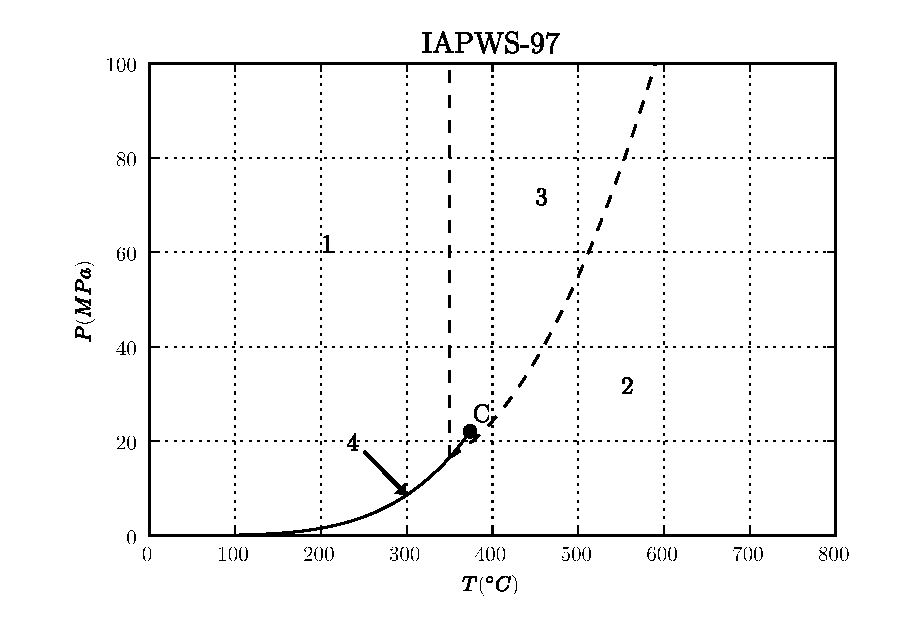
\includegraphics{ptplot.eps}
    \caption{Operating range of the IAPWS-97 thermodynamic formulation}
    \label{fg:iapws97_range}
  \end{center}
\end {figure}

The \texttt{IAPWS97} library can be imported using the command:

\begin{verbatim} 
   from IAPWS97 import *
\end{verbatim}

The functions available through the \texttt{IAPWS97} library are listed in Table \ref{tb:iapws97_functions} and described below.

\begin{table}
  \begin{center}
    \begin{tabular}{|l|l|p{65mm}|}
      \hline
      \textbf{Function} & \textbf{Type} & \textbf{Description}\\
      \hline
      \hyperref[sec:iapws97:b23p]{\texttt{b23p}} & float & pressure on boundary between steam and supercritical regions, as a function of temperature\\
      \hyperref[sec:iapws97:b23t]{\texttt{b23t}} & float & temperature on boundary between steam and supercritical regions, as a function of pressure\\
      \hyperref[sec:iapws97:cowat]{\texttt{cowat}} & tuple & density and internal energy of liquid water\\
      \hyperref[sec:iapws97:density_temperature_plot]{\texttt{density\_temperature\_plot}} & -- & draws region boundaries on a density-temperature plot\\
      \hyperref[sec:iapws97:pressure_temperature_plot]{\texttt{pressure\_temperature\_plot}} & -- & draws region boundaries on a pressure-temperature plot\\
      \hyperref[sec:iapws97:sat]{\texttt{sat}} & float & saturation pressure as a function of temperature\\
      \hyperref[sec:iapws97:super]{\texttt{super}} & tuple & pressure and internal energy of supercritical fluid\\
      \hyperref[sec:iapws97:supst]{\texttt{supst}} & tuple & density and internal energy of dry steam\\
      \hyperref[sec:iapws97:test]{\texttt{test}} & -- & prints results of verification tests from \cite{iapws_2000}\\
      \hyperref[sec:iapws97:tsat]{\texttt{tsat}} & float & saturation temperature as a function of pressure\\
      \hyperref[sec:iapws97:visc]{\texttt{visc}} & float & dynamic viscosity of water, steam or supercritical fluid\\
      \hline
    \end{tabular}
    \caption{\texttt{IAPWS97} functions}
    \label{tb:iapws97_functions}
  \end{center}
\end{table}

\section{Thermodynamic functions}

The IAPWS-97 formulation provides thermodynamic functions for liquid water, dry steam and supercritical fluid.  These functions calculate secondary parameters from the primary thermodynamic variables.

\begin{snugshade}
\subsection{Liquid water: \texttt{cowat(\emph{t,p})}}
\end{snugshade}
\label{sec:iapws97:cowat}

The \texttt{cowat} function returns a two-element tuple (\texttt{d},\texttt{u}) of density (kg/m$^3$) and internal energy (J/kg) of liquid water as a function of temperature \texttt{t} ($^{\circ}$C) and pressure \texttt{p} (Pa).

\textbf{Parameters:}
\begin{itemize}
\item \textbf{t}: float\\
  Temperature ($^{\circ}$C)
\item \textbf{p}: float\\
  Pressure (Pa)
\end{itemize}

\begin{snugshade}
\subsection{Dry steam: \texttt{supst(\emph{t,p})}}
\end{snugshade}
\label{sec:iapws97:supst}

The \texttt{supst} function returns a two-element tuple (\texttt{d},\texttt{u}) of density (kg/m$^3$) and internal energy (J/kg) of dry steam as a function of temperature \texttt{t} ($^{\circ}$C) and pressure \texttt{p} (Pa).

\textbf{Parameters:}
\begin{itemize}
\item \textbf{t}: float\\
  Temperature ($^{\circ}$C)
\item \textbf{p}: float\\
  Pressure (Pa)
\end{itemize}

\begin{snugshade}
\subsection{Supercritical fluid: \texttt{super(\emph{d,t})}}
\end{snugshade}
\label{sec:iapws97:super}

The \texttt{super} function returns a two-element tuple (\texttt{p},\texttt{u}) of pressure (Pa) and internal energy (J/kg) of supercritical fluid as a function of density \texttt{d} (kg/m$^3$) and temperature \texttt{t} ($^{\circ}$C).

\textbf{Parameters:}
\begin{itemize}
\item \textbf{d}: float\\
  Density (kg/m$^3$)
\item \textbf{t}: float\\
  Temperature ($^{\circ}$C)
\end{itemize}

\begin{snugshade}
\section{Viscosity: \texttt{visc(\emph{d,t})}}
\end{snugshade}
\label{sec:iapws97:visc}

The \texttt{visc} function returns the dynamic viscosity (Pa.s) of liquid water, dry steam or supercritical fluid as a function of density \texttt{d} (kg/m$^3$) and temperature \texttt{t} ($^{\circ}$C).  This function is based on the supplementary ``IAPWS Formulation 2008 for the Viscosity of Ordinary Water Substance'', without the critical enhancement of viscosity near the critical point.

\textbf{Parameters:}
\begin{itemize}
\item \textbf{d}: float\\
  Density (kg/m$^3$)
\item \textbf{t}: float\\
  Temperature ($^{\circ}$C)
\end{itemize}

\section{Region boundaries}

These functions describe the boundaries between the four thermodynamic regions of the IAPWS-97 formulation (see Figure \ref{fg:iapws97_range}).  There is no equation for the boundary between regions 1 and 3 as this is simply the line $T = 350 ^{\circ}$C.

\subsection{Saturation line: \texttt{sat(\emph{t})} and \texttt{tsat(\emph{p})}}

\begin{snugshade}
\subsubsection{\texttt{sat(\emph{t})}}
\end{snugshade}
\label{sec:iapws97:sat}

The \texttt{sat} function returns the saturation pressure (Pa) at a given temperature \texttt{t} ($^{\circ}$C), for temperatures below the critical temperature.

\textbf{Parameters:}
\begin{itemize}
\item \textbf{t}: float\\
  Temperature ($^{\circ}$C)
\end{itemize}

\begin{snugshade}
\subsubsection{\texttt{tsat(\emph{p})}}
\end{snugshade}
\label{sec:iapws97:tsat}

The \texttt{tsat} function returns the saturation temperature ($^{\circ}$C) at a given pressure \texttt{p} (Pa), for pressures below the critical pressure.

\textbf{Parameters:}
\begin{itemize}
\item \textbf{p}: float\\
  Pressure (Pa)
\end{itemize}

\subsection{Steam/supercritical boundary}
\label{region23_boundary}

\begin{snugshade}
\subsubsection{\texttt{b23p(\emph{t})}}
\end{snugshade}
\label{sec:iapws97:b23p}

The \texttt{b23p} function returns the pressure (Pa) on the boundary of the dry steam and supercritical regions (regions 2 and 3) at a given temperature \texttt{t} ($^{\circ}$C).

\textbf{Parameters:}
\begin{itemize}
\item \textbf{t}: float\\
  Temperature ($^{\circ}$C)
\end{itemize}

\begin{snugshade}
\subsubsection{\texttt{b23t(\emph{p})}}
\end{snugshade}
\label{sec:iapws97:b23t}

The \texttt{b23t} function returns the temperature ($^{\circ}$C) on the boundary of the dry steam and supercritical regions (regions 2 and 3) at a given pressure \texttt{p} (Pa).

\textbf{Parameters:}
\begin{itemize}
\item \textbf{p}: float\\
  Pressure (Pa)
\end{itemize}

\section{Plotting functions}

The \texttt{IAPWS97} library contains two functions used for including the IAPWS-97 thermodynamic region boundaries on plots.

\begin{snugshade}
\subsection{\texttt{pressure\_temperature\_plot(\emph{plt})}}
\end{snugshade}
\label{sec:iapws97:pressure_temperature_plot}

Draws the IAPWS-97 thermodynamic region boundaries on a pressure-temperature diagram.

\textbf{Parameters:}
\begin{itemize}
\item \textbf{plt}: \texttt{matplotlib.pyplot} instance\\
  An instance of the \texttt{matplotlib.pyplot} library, imported in the calling script using e.g. \texttt{import matplotlib.pyplot as plt}.
\end{itemize}

\begin{snugshade}
\subsection{\texttt{density\_temperature\_plot(\emph{plt})}}
\end{snugshade}
\label{sec:iapws97:density_temperature_plot}

Draws the IAPWS-97 thermodynamic region boundaries on a density-temperature diagram.  (This function requires the Scientific Python (\texttt{scipy}) library to be installed.)

\textbf{Parameters:}
\begin{itemize}
\item \textbf{plt}: \texttt{matplotlib.pyplot} instance\\
  An instance of the \texttt{matplotlib.pyplot} library, imported in the calling script using e.g. \texttt{import matplotlib.pyplot as plt}.
\end{itemize}

\begin{snugshade}
\section{Testing: \texttt{test()}}
\end{snugshade}
\label{sec:iapws97:test}

The \texttt{test} function prints the results of the verification tests in \cite{iapws_2000} for the \texttt{cowat}, \texttt{supst} and \texttt{super} functions.

%------------------------------------------------------------------------
\renewcommand\bibname{References} % rather than 'Bibliography'
\bibliographystyle{PyTOUGH}
\addcontentsline{toc}{chapter}{References} % adds to table of contents
\bibliography{PyTOUGH}

%------------------------------------------------------------------------

\end{document}
